\documentclass[11pt]{article}

    \usepackage[breakable]{tcolorbox}
    \usepackage{parskip} % Stop auto-indenting (to mimic markdown behaviour)
    \usepackage{bm}
    \usepackage{hyperref} 
\usepackage{makecell}
    \usepackage{iftex}
    \ifPDFTeX
    	\usepackage[T1]{fontenc}
    	\usepackage{mathpazo}
    \else
    	\usepackage{fontspec}
    \fi

	\usepackage{titling}

    % Basic figure setup, for now with no caption control since it's done
    % automatically by Pandoc (which extracts ![](path) syntax from Markdown).
    \usepackage{graphicx}
    % Maintain compatibility with old templates. Remove in nbconvert 6.0
    \let\Oldincludegraphics\includegraphics
    % Ensure that by default, figures have no caption (until we provide a
    % proper Figure object with a Caption API and a way to capture that
    % in the conversion process - todo).
    \usepackage{caption}
    \DeclareCaptionFormat{nocaption}{}
    \captionsetup{format=nocaption,aboveskip=0pt,belowskip=0pt}

    \usepackage[Export]{adjustbox} % Used to constrain images to a maximum size
    \adjustboxset{max size={0.9\linewidth}{0.9\paperheight}}
    \usepackage{float}
    \floatplacement{figure}{H} % forces figures to be placed at the correct location
    \usepackage{xcolor} % Allow colors to be defined
    \usepackage{enumerate} % Needed for markdown enumerations to work
    \usepackage{geometry} % Used to adjust the document margins
    \usepackage{amsmath} % Equations
    \usepackage{amssymb} % Equations
    \usepackage{textcomp} % defines textquotesingle
    % Hack from http://tex.stackexchange.com/a/47451/13684:
    \AtBeginDocument{%
        \def\PYZsq{\textquotesingle}% Upright quotes in Pygmentized code
    }
    \usepackage{upquote} % Upright quotes for verbatim code
    \usepackage{eurosym} % defines \euro
    \usepackage[mathletters]{ucs} % Extended unicode (utf-8) support
    \usepackage{fancyvrb} % verbatim replacement that allows latex
    \usepackage{grffile} % extends the file name processing of package graphics 
                         % to support a larger range
    \makeatletter % fix for grffile with XeLaTeX
    \def\Gread@@xetex#1{%
      \IfFileExists{"\Gin@base".bb}%
      {\Gread@eps{\Gin@base.bb}}%
      {\Gread@@xetex@aux#1}%
    }
    \makeatother

    % The hyperref package gives us a pdf with properly built
    % internal navigation ('pdf bookmarks' for the table of contents,
    % internal cross-reference links, web links for URLs, etc.)
    \usepackage{hyperref}
    % The default LaTeX title has an obnoxious amount of whitespace. By default,
    % titling removes some of it. It also provides customization options.
    \usepackage{titling}
    \usepackage{longtable} % longtable support required by pandoc >1.10
    \usepackage{booktabs}  % table support for pandoc > 1.12.2
    \usepackage[inline]{enumitem} % IRkernel/repr support (it uses the enumerate* environment)
    \usepackage[normalem]{ulem} % ulem is needed to support strikethroughs (\sout)
                                % normalem makes italics be italics, not underlines
    \usepackage{mathrsfs}
    
    
    % Colors for the hyperref package
    \definecolor{urlcolor}{rgb}{0,.145,.698}
    \definecolor{linkcolor}{rgb}{.71,0.21,0.01}
    \definecolor{citecolor}{rgb}{.12,.54,.11}

    % ANSI colors
    \definecolor{ansi-black}{HTML}{3E424D}
    \definecolor{ansi-black-intense}{HTML}{282C36}
    \definecolor{ansi-red}{HTML}{E75C58}
    \definecolor{ansi-red-intense}{HTML}{B22B31}
    \definecolor{ansi-green}{HTML}{00A250}
    \definecolor{ansi-green-intense}{HTML}{007427}
    \definecolor{ansi-yellow}{HTML}{DDB62B}
    \definecolor{ansi-yellow-intense}{HTML}{B27D12}
    \definecolor{ansi-blue}{HTML}{208FFB}
    \definecolor{ansi-blue-intense}{HTML}{0065CA}
    \definecolor{ansi-magenta}{HTML}{D160C4}
    \definecolor{ansi-magenta-intense}{HTML}{A03196}
    \definecolor{ansi-cyan}{HTML}{60C6C8}
    \definecolor{ansi-cyan-intense}{HTML}{258F8F}
    \definecolor{ansi-white}{HTML}{C5C1B4}
    \definecolor{ansi-white-intense}{HTML}{A1A6B2}
    \definecolor{ansi-default-inverse-fg}{HTML}{FFFFFF}
    \definecolor{ansi-default-inverse-bg}{HTML}{000000}

    % commands and environments needed by pandoc snippets
    % extracted from the output of `pandoc -s`
    \providecommand{\tightlist}{%
      \setlength{\itemsep}{0pt}\setlength{\parskip}{0pt}}
    \DefineVerbatimEnvironment{Highlighting}{Verbatim}{commandchars=\\\{\}}
    % Add ',fontsize=\small' for more characters per line
    \newenvironment{Shaded}{}{}
    \newcommand{\KeywordTok}[1]{\textcolor[rgb]{0.00,0.44,0.13}{\textbf{{#1}}}}
    \newcommand{\DataTypeTok}[1]{\textcolor[rgb]{0.56,0.13,0.00}{{#1}}}
    \newcommand{\DecValTok}[1]{\textcolor[rgb]{0.25,0.63,0.44}{{#1}}}
    \newcommand{\BaseNTok}[1]{\textcolor[rgb]{0.25,0.63,0.44}{{#1}}}
    \newcommand{\FloatTok}[1]{\textcolor[rgb]{0.25,0.63,0.44}{{#1}}}
    \newcommand{\CharTok}[1]{\textcolor[rgb]{0.25,0.44,0.63}{{#1}}}
    \newcommand{\StringTok}[1]{\textcolor[rgb]{0.25,0.44,0.63}{{#1}}}
    \newcommand{\CommentTok}[1]{\textcolor[rgb]{0.38,0.63,0.69}{\textit{{#1}}}}
    \newcommand{\OtherTok}[1]{\textcolor[rgb]{0.00,0.44,0.13}{{#1}}}
    \newcommand{\AlertTok}[1]{\textcolor[rgb]{1.00,0.00,0.00}{\textbf{{#1}}}}
    \newcommand{\FunctionTok}[1]{\textcolor[rgb]{0.02,0.16,0.49}{{#1}}}
    \newcommand{\RegionMarkerTok}[1]{{#1}}
    \newcommand{\ErrorTok}[1]{\textcolor[rgb]{1.00,0.00,0.00}{\textbf{{#1}}}}
    \newcommand{\NormalTok}[1]{{#1}}
    
    % Additional commands for more recent versions of Pandoc
    \newcommand{\ConstantTok}[1]{\textcolor[rgb]{0.53,0.00,0.00}{{#1}}}
    \newcommand{\SpecialCharTok}[1]{\textcolor[rgb]{0.25,0.44,0.63}{{#1}}}
    \newcommand{\VerbatimStringTok}[1]{\textcolor[rgb]{0.25,0.44,0.63}{{#1}}}
    \newcommand{\SpecialStringTok}[1]{\textcolor[rgb]{0.73,0.40,0.53}{{#1}}}
    \newcommand{\ImportTok}[1]{{#1}}
    \newcommand{\DocumentationTok}[1]{\textcolor[rgb]{0.73,0.13,0.13}{\textit{{#1}}}}
    \newcommand{\AnnotationTok}[1]{\textcolor[rgb]{0.38,0.63,0.69}{\textbf{\textit{{#1}}}}}
    \newcommand{\CommentVarTok}[1]{\textcolor[rgb]{0.38,0.63,0.69}{\textbf{\textit{{#1}}}}}
    \newcommand{\VariableTok}[1]{\textcolor[rgb]{0.10,0.09,0.49}{{#1}}}
    \newcommand{\ControlFlowTok}[1]{\textcolor[rgb]{0.00,0.44,0.13}{\textbf{{#1}}}}
    \newcommand{\OperatorTok}[1]{\textcolor[rgb]{0.40,0.40,0.40}{{#1}}}
    \newcommand{\BuiltInTok}[1]{{#1}}
    \newcommand{\ExtensionTok}[1]{{#1}}
    \newcommand{\PreprocessorTok}[1]{\textcolor[rgb]{0.74,0.48,0.00}{{#1}}}
    \newcommand{\AttributeTok}[1]{\textcolor[rgb]{0.49,0.56,0.16}{{#1}}}
    \newcommand{\InformationTok}[1]{\textcolor[rgb]{0.38,0.63,0.69}{\textbf{\textit{{#1}}}}}
    \newcommand{\WarningTok}[1]{\textcolor[rgb]{0.38,0.63,0.69}{\textbf{\textit{{#1}}}}}
    
    
    % Define a nice break command that doesn't care if a line doesn't already
    % exist.
    \def\br{\hspace*{\fill} \\* }
    % Math Jax compatibility definitions
    \def\gt{>}
    \def\lt{<}
    \let\Oldtex\TeX
    \let\Oldlatex\LaTeX
    \renewcommand{\TeX}{\textrm{\Oldtex}}
    \renewcommand{\LaTeX}{\textrm{\Oldlatex}}
    % Document parameters
    % Document title
%    \title{\huge Exasim: Partial Differential Equation Application Builder For Extreme Scalable Simulations }
        
%   \author{\Large N. C. Nguyen \\[2ex]}
    \date{}
    
% Pygments definitions
\makeatletter
\def\PY@reset{\let\PY@it=\relax \let\PY@bf=\relax%
    \let\PY@ul=\relax \let\PY@tc=\relax%
    \let\PY@bc=\relax \let\PY@ff=\relax}
\def\PY@tok#1{\csname PY@tok@#1\endcsname}
\def\PY@toks#1+{\ifx\relax#1\empty\else%
    \PY@tok{#1}\expandafter\PY@toks\fi}
\def\PY@do#1{\PY@bc{\PY@tc{\PY@ul{%
    \PY@it{\PY@bf{\PY@ff{#1}}}}}}}
\def\PY#1#2{\PY@reset\PY@toks#1+\relax+\PY@do{#2}}

\expandafter\def\csname PY@tok@w\endcsname{\def\PY@tc##1{\textcolor[rgb]{0.73,0.73,0.73}{##1}}}
\expandafter\def\csname PY@tok@c\endcsname{\let\PY@it=\textit\def\PY@tc##1{\textcolor[rgb]{0.25,0.50,0.50}{##1}}}
\expandafter\def\csname PY@tok@cp\endcsname{\def\PY@tc##1{\textcolor[rgb]{0.74,0.48,0.00}{##1}}}
\expandafter\def\csname PY@tok@k\endcsname{\let\PY@bf=\textbf\def\PY@tc##1{\textcolor[rgb]{0.00,0.50,0.00}{##1}}}
\expandafter\def\csname PY@tok@kp\endcsname{\def\PY@tc##1{\textcolor[rgb]{0.00,0.50,0.00}{##1}}}
\expandafter\def\csname PY@tok@kt\endcsname{\def\PY@tc##1{\textcolor[rgb]{0.69,0.00,0.25}{##1}}}
\expandafter\def\csname PY@tok@o\endcsname{\def\PY@tc##1{\textcolor[rgb]{0.40,0.40,0.40}{##1}}}
\expandafter\def\csname PY@tok@ow\endcsname{\let\PY@bf=\textbf\def\PY@tc##1{\textcolor[rgb]{0.67,0.13,1.00}{##1}}}
\expandafter\def\csname PY@tok@nb\endcsname{\def\PY@tc##1{\textcolor[rgb]{0.00,0.50,0.00}{##1}}}
\expandafter\def\csname PY@tok@nf\endcsname{\def\PY@tc##1{\textcolor[rgb]{0.00,0.00,1.00}{##1}}}
\expandafter\def\csname PY@tok@nc\endcsname{\let\PY@bf=\textbf\def\PY@tc##1{\textcolor[rgb]{0.00,0.00,1.00}{##1}}}
\expandafter\def\csname PY@tok@nn\endcsname{\let\PY@bf=\textbf\def\PY@tc##1{\textcolor[rgb]{0.00,0.00,1.00}{##1}}}
\expandafter\def\csname PY@tok@ne\endcsname{\let\PY@bf=\textbf\def\PY@tc##1{\textcolor[rgb]{0.82,0.25,0.23}{##1}}}
\expandafter\def\csname PY@tok@nv\endcsname{\def\PY@tc##1{\textcolor[rgb]{0.10,0.09,0.49}{##1}}}
\expandafter\def\csname PY@tok@no\endcsname{\def\PY@tc##1{\textcolor[rgb]{0.53,0.00,0.00}{##1}}}
\expandafter\def\csname PY@tok@nl\endcsname{\def\PY@tc##1{\textcolor[rgb]{0.63,0.63,0.00}{##1}}}
\expandafter\def\csname PY@tok@ni\endcsname{\let\PY@bf=\textbf\def\PY@tc##1{\textcolor[rgb]{0.60,0.60,0.60}{##1}}}
\expandafter\def\csname PY@tok@na\endcsname{\def\PY@tc##1{\textcolor[rgb]{0.49,0.56,0.16}{##1}}}
\expandafter\def\csname PY@tok@nt\endcsname{\let\PY@bf=\textbf\def\PY@tc##1{\textcolor[rgb]{0.00,0.50,0.00}{##1}}}
\expandafter\def\csname PY@tok@nd\endcsname{\def\PY@tc##1{\textcolor[rgb]{0.67,0.13,1.00}{##1}}}
\expandafter\def\csname PY@tok@s\endcsname{\def\PY@tc##1{\textcolor[rgb]{0.73,0.13,0.13}{##1}}}
\expandafter\def\csname PY@tok@sd\endcsname{\let\PY@it=\textit\def\PY@tc##1{\textcolor[rgb]{0.73,0.13,0.13}{##1}}}
\expandafter\def\csname PY@tok@si\endcsname{\let\PY@bf=\textbf\def\PY@tc##1{\textcolor[rgb]{0.73,0.40,0.53}{##1}}}
\expandafter\def\csname PY@tok@se\endcsname{\let\PY@bf=\textbf\def\PY@tc##1{\textcolor[rgb]{0.73,0.40,0.13}{##1}}}
\expandafter\def\csname PY@tok@sr\endcsname{\def\PY@tc##1{\textcolor[rgb]{0.73,0.40,0.53}{##1}}}
\expandafter\def\csname PY@tok@ss\endcsname{\def\PY@tc##1{\textcolor[rgb]{0.10,0.09,0.49}{##1}}}
\expandafter\def\csname PY@tok@sx\endcsname{\def\PY@tc##1{\textcolor[rgb]{0.00,0.50,0.00}{##1}}}
\expandafter\def\csname PY@tok@m\endcsname{\def\PY@tc##1{\textcolor[rgb]{0.40,0.40,0.40}{##1}}}
\expandafter\def\csname PY@tok@gh\endcsname{\let\PY@bf=\textbf\def\PY@tc##1{\textcolor[rgb]{0.00,0.00,0.50}{##1}}}
\expandafter\def\csname PY@tok@gu\endcsname{\let\PY@bf=\textbf\def\PY@tc##1{\textcolor[rgb]{0.50,0.00,0.50}{##1}}}
\expandafter\def\csname PY@tok@gd\endcsname{\def\PY@tc##1{\textcolor[rgb]{0.63,0.00,0.00}{##1}}}
\expandafter\def\csname PY@tok@gi\endcsname{\def\PY@tc##1{\textcolor[rgb]{0.00,0.63,0.00}{##1}}}
\expandafter\def\csname PY@tok@gr\endcsname{\def\PY@tc##1{\textcolor[rgb]{1.00,0.00,0.00}{##1}}}
\expandafter\def\csname PY@tok@ge\endcsname{\let\PY@it=\textit}
\expandafter\def\csname PY@tok@gs\endcsname{\let\PY@bf=\textbf}
\expandafter\def\csname PY@tok@gp\endcsname{\let\PY@bf=\textbf\def\PY@tc##1{\textcolor[rgb]{0.00,0.00,0.50}{##1}}}
\expandafter\def\csname PY@tok@go\endcsname{\def\PY@tc##1{\textcolor[rgb]{0.53,0.53,0.53}{##1}}}
\expandafter\def\csname PY@tok@gt\endcsname{\def\PY@tc##1{\textcolor[rgb]{0.00,0.27,0.87}{##1}}}
\expandafter\def\csname PY@tok@err\endcsname{\def\PY@bc##1{\setlength{\fboxsep}{0pt}\fcolorbox[rgb]{1.00,0.00,0.00}{1,1,1}{\strut ##1}}}
\expandafter\def\csname PY@tok@kc\endcsname{\let\PY@bf=\textbf\def\PY@tc##1{\textcolor[rgb]{0.00,0.50,0.00}{##1}}}
\expandafter\def\csname PY@tok@kd\endcsname{\let\PY@bf=\textbf\def\PY@tc##1{\textcolor[rgb]{0.00,0.50,0.00}{##1}}}
\expandafter\def\csname PY@tok@kn\endcsname{\let\PY@bf=\textbf\def\PY@tc##1{\textcolor[rgb]{0.00,0.50,0.00}{##1}}}
\expandafter\def\csname PY@tok@kr\endcsname{\let\PY@bf=\textbf\def\PY@tc##1{\textcolor[rgb]{0.00,0.50,0.00}{##1}}}
\expandafter\def\csname PY@tok@bp\endcsname{\def\PY@tc##1{\textcolor[rgb]{0.00,0.50,0.00}{##1}}}
\expandafter\def\csname PY@tok@fm\endcsname{\def\PY@tc##1{\textcolor[rgb]{0.00,0.00,1.00}{##1}}}
\expandafter\def\csname PY@tok@vc\endcsname{\def\PY@tc##1{\textcolor[rgb]{0.10,0.09,0.49}{##1}}}
\expandafter\def\csname PY@tok@vg\endcsname{\def\PY@tc##1{\textcolor[rgb]{0.10,0.09,0.49}{##1}}}
\expandafter\def\csname PY@tok@vi\endcsname{\def\PY@tc##1{\textcolor[rgb]{0.10,0.09,0.49}{##1}}}
\expandafter\def\csname PY@tok@vm\endcsname{\def\PY@tc##1{\textcolor[rgb]{0.10,0.09,0.49}{##1}}}
\expandafter\def\csname PY@tok@sa\endcsname{\def\PY@tc##1{\textcolor[rgb]{0.73,0.13,0.13}{##1}}}
\expandafter\def\csname PY@tok@sb\endcsname{\def\PY@tc##1{\textcolor[rgb]{0.73,0.13,0.13}{##1}}}
\expandafter\def\csname PY@tok@sc\endcsname{\def\PY@tc##1{\textcolor[rgb]{0.73,0.13,0.13}{##1}}}
\expandafter\def\csname PY@tok@dl\endcsname{\def\PY@tc##1{\textcolor[rgb]{0.73,0.13,0.13}{##1}}}
\expandafter\def\csname PY@tok@s2\endcsname{\def\PY@tc##1{\textcolor[rgb]{0.73,0.13,0.13}{##1}}}
\expandafter\def\csname PY@tok@sh\endcsname{\def\PY@tc##1{\textcolor[rgb]{0.73,0.13,0.13}{##1}}}
\expandafter\def\csname PY@tok@s1\endcsname{\def\PY@tc##1{\textcolor[rgb]{0.73,0.13,0.13}{##1}}}
\expandafter\def\csname PY@tok@mb\endcsname{\def\PY@tc##1{\textcolor[rgb]{0.40,0.40,0.40}{##1}}}
\expandafter\def\csname PY@tok@mf\endcsname{\def\PY@tc##1{\textcolor[rgb]{0.40,0.40,0.40}{##1}}}
\expandafter\def\csname PY@tok@mh\endcsname{\def\PY@tc##1{\textcolor[rgb]{0.40,0.40,0.40}{##1}}}
\expandafter\def\csname PY@tok@mi\endcsname{\def\PY@tc##1{\textcolor[rgb]{0.40,0.40,0.40}{##1}}}
\expandafter\def\csname PY@tok@il\endcsname{\def\PY@tc##1{\textcolor[rgb]{0.40,0.40,0.40}{##1}}}
\expandafter\def\csname PY@tok@mo\endcsname{\def\PY@tc##1{\textcolor[rgb]{0.40,0.40,0.40}{##1}}}
\expandafter\def\csname PY@tok@ch\endcsname{\let\PY@it=\textit\def\PY@tc##1{\textcolor[rgb]{0.25,0.50,0.50}{##1}}}
\expandafter\def\csname PY@tok@cm\endcsname{\let\PY@it=\textit\def\PY@tc##1{\textcolor[rgb]{0.25,0.50,0.50}{##1}}}
\expandafter\def\csname PY@tok@cpf\endcsname{\let\PY@it=\textit\def\PY@tc##1{\textcolor[rgb]{0.25,0.50,0.50}{##1}}}
\expandafter\def\csname PY@tok@c1\endcsname{\let\PY@it=\textit\def\PY@tc##1{\textcolor[rgb]{0.25,0.50,0.50}{##1}}}
\expandafter\def\csname PY@tok@cs\endcsname{\let\PY@it=\textit\def\PY@tc##1{\textcolor[rgb]{0.25,0.50,0.50}{##1}}}

\def\PYZbs{\char`\\}
\def\PYZus{\char`\_}
\def\PYZob{\char`\{}
\def\PYZcb{\char`\}}
\def\PYZca{\char`\^}
\def\PYZam{\char`\&}
\def\PYZlt{\char`\<}
\def\PYZgt{\char`\>}
\def\PYZsh{\char`\#}
\def\PYZpc{\char`\%}
\def\PYZdl{\char`\$}
\def\PYZhy{\char`\-}
\def\PYZsq{\char`\'}
\def\PYZdq{\char`\"}
\def\PYZti{\char`\~}
% for compatibility with earlier versions
\def\PYZat{@}
\def\PYZlb{[}
\def\PYZrb{]}
\makeatother


    % For linebreaks inside Verbatim environment from package fancyvrb. 
    \makeatletter
        \newbox\Wrappedcontinuationbox 
        \newbox\Wrappedvisiblespacebox 
        \newcommand*\Wrappedvisiblespace {\textcolor{red}{\textvisiblespace}} 
        \newcommand*\Wrappedcontinuationsymbol {\textcolor{red}{\llap{\tiny$\m@th\hookrightarrow$}}} 
        \newcommand*\Wrappedcontinuationindent {3ex } 
        \newcommand*\Wrappedafterbreak {\kern\Wrappedcontinuationindent\copy\Wrappedcontinuationbox} 
        % Take advantage of the already applied Pygments mark-up to insert 
        % potential linebreaks for TeX processing. 
        %        {, <, #, %, $, ' and ": go to next line. 
        %        _, }, ^, &, >, - and ~: stay at end of broken line. 
        % Use of \textquotesingle for straight quote. 
        \newcommand*\Wrappedbreaksatspecials {% 
            \def\PYGZus{\discretionary{\char`\_}{\Wrappedafterbreak}{\char`\_}}% 
            \def\PYGZob{\discretionary{}{\Wrappedafterbreak\char`\{}{\char`\{}}% 
            \def\PYGZcb{\discretionary{\char`\}}{\Wrappedafterbreak}{\char`\}}}% 
            \def\PYGZca{\discretionary{\char`\^}{\Wrappedafterbreak}{\char`\^}}% 
            \def\PYGZam{\discretionary{\char`\&}{\Wrappedafterbreak}{\char`\&}}% 
            \def\PYGZlt{\discretionary{}{\Wrappedafterbreak\char`\<}{\char`\<}}% 
            \def\PYGZgt{\discretionary{\char`\>}{\Wrappedafterbreak}{\char`\>}}% 
            \def\PYGZsh{\discretionary{}{\Wrappedafterbreak\char`\#}{\char`\#}}% 
            \def\PYGZpc{\discretionary{}{\Wrappedafterbreak\char`\%}{\char`\%}}% 
            \def\PYGZdl{\discretionary{}{\Wrappedafterbreak\char`\$}{\char`\$}}% 
            \def\PYGZhy{\discretionary{\char`\-}{\Wrappedafterbreak}{\char`\-}}% 
            \def\PYGZsq{\discretionary{}{\Wrappedafterbreak\textquotesingle}{\textquotesingle}}% 
            \def\PYGZdq{\discretionary{}{\Wrappedafterbreak\char`\"}{\char`\"}}% 
            \def\PYGZti{\discretionary{\char`\~}{\Wrappedafterbreak}{\char`\~}}% 
        } 
        % Some characters . , ; ? ! / are not pygmentized. 
        % This macro makes them "active" and they will insert potential linebreaks 
        \newcommand*\Wrappedbreaksatpunct {% 
            \lccode`\~`\.\lowercase{\def~}{\discretionary{\hbox{\char`\.}}{\Wrappedafterbreak}{\hbox{\char`\.}}}% 
            \lccode`\~`\,\lowercase{\def~}{\discretionary{\hbox{\char`\,}}{\Wrappedafterbreak}{\hbox{\char`\,}}}% 
            \lccode`\~`\;\lowercase{\def~}{\discretionary{\hbox{\char`\;}}{\Wrappedafterbreak}{\hbox{\char`\;}}}% 
            \lccode`\~`\:\lowercase{\def~}{\discretionary{\hbox{\char`\:}}{\Wrappedafterbreak}{\hbox{\char`\:}}}% 
            \lccode`\~`\?\lowercase{\def~}{\discretionary{\hbox{\char`\?}}{\Wrappedafterbreak}{\hbox{\char`\?}}}% 
            \lccode`\~`\!\lowercase{\def~}{\discretionary{\hbox{\char`\!}}{\Wrappedafterbreak}{\hbox{\char`\!}}}% 
            \lccode`\~`\/\lowercase{\def~}{\discretionary{\hbox{\char`\/}}{\Wrappedafterbreak}{\hbox{\char`\/}}}% 
            \catcode`\.\active
            \catcode`\,\active 
            \catcode`\;\active
            \catcode`\:\active
            \catcode`\?\active
            \catcode`\!\active
            \catcode`\/\active 
            \lccode`\~`\~ 	
        }
    \makeatother

    \let\OriginalVerbatim=\Verbatim
    \makeatletter
    \renewcommand{\Verbatim}[1][1]{%
        %\parskip\z@skip
        \sbox\Wrappedcontinuationbox {\Wrappedcontinuationsymbol}%
        \sbox\Wrappedvisiblespacebox {\FV@SetupFont\Wrappedvisiblespace}%
        \def\FancyVerbFormatLine ##1{\hsize\linewidth
            \vtop{\raggedright\hyphenpenalty\z@\exhyphenpenalty\z@
                \doublehyphendemerits\z@\finalhyphendemerits\z@
                \strut ##1\strut}%
        }%
        % If the linebreak is at a space, the latter will be displayed as visible
        % space at end of first line, and a continuation symbol starts next line.
        % Stretch/shrink are however usually zero for typewriter font.
        \def\FV@Space {%
            \nobreak\hskip\z@ plus\fontdimen3\font minus\fontdimen4\font
            \discretionary{\copy\Wrappedvisiblespacebox}{\Wrappedafterbreak}
            {\kern\fontdimen2\font}%
        }%
        
        % Allow breaks at special characters using \PYG... macros.
        \Wrappedbreaksatspecials
        % Breaks at punctuation characters . , ; ? ! and / need catcode=\active 	
        \OriginalVerbatim[#1,codes*=\Wrappedbreaksatpunct]%
    }
    \makeatother

    % Exact colors from NB
    \definecolor{incolor}{HTML}{303F9F}
    \definecolor{outcolor}{HTML}{D84315}
    \definecolor{cellborder}{HTML}{CFCFCF}
    \definecolor{cellbackground}{HTML}{F7F7F7}
    
    % prompt
    \makeatletter
    \newcommand{\boxspacing}{\kern\kvtcb@left@rule\kern\kvtcb@boxsep}
    \makeatother
    \newcommand{\prompt}[4]{
        \ttfamily\llap{{\color{#2}[#3]:\hspace{3pt}#4}}\vspace{-\baselineskip}
    }
    

    
    % Prevent overflowing lines due to hard-to-break entities
    \sloppy 
    % Setup hyperref package
    \hypersetup{
      breaklinks=true,  % so long urls are correctly broken across lines
      colorlinks=true,
      urlcolor=urlcolor,
      linkcolor=linkcolor,
      citecolor=citecolor,
      }
    % Slightly bigger margins than the latex defaults
    
    \geometry{verbose,tmargin=1in,bmargin=1in,lmargin=1in,rmargin=1in}
    
    
\pretitle{%
  \begin{center}
  \LARGE
  
\includegraphics[scale=1]{exasimlogosmall.png}\\[\bigskipamount]
}
\posttitle{\end{center}}    

\begin{document}
    
        \title{\huge Generating Discontinuous Galerkin Codes For Extreme Scalable Simulations}
        
    \maketitle

 \rule{16.4cm}{0.25cm} 

\hspace{8cm} {\large The documentation for Exasim 0.2}

\hspace{8cm}    {\large Developed and written by N. C. Nguyen}

\hspace{8cm}   {\large Designed by N. C. Nguyen and J. Peraire}
        
\hspace{8cm} {\large \today}
    
\vspace{6cm}

%Acknowledgment: We thank our students, postdocs, academic and industrial collaborators.  We are Professor Bernardo Cockburn,    
    
    \newpage
    
\section{Overview}

\texttt{Exasim} is an open-source software for generating discontinuous Galerkin codes to numerically solve {\em parametrized} partial differential equations (PDEs) on different computing platforms with distributed memory.  It combines high-level languages  and low-level languages to easily construct {\em parametrized} PDE models and automatically produce high-performance C++ codes. The construction of {\em parametrized} PDE models and the generation of the stand-alone C++ production code are handled by high-level languages, while the production code itself can run on various machines, from laptops to the largest supercomputers, with both CPU and GPU processors. Figure 1 illustrates  the intended use of \texttt{Exasim} for solving PDEs.

%\texttt{Exasim} makes building PDE solvers as simple as writing PDE models in Latex.

\begin{figure}[th]
\begin{center}
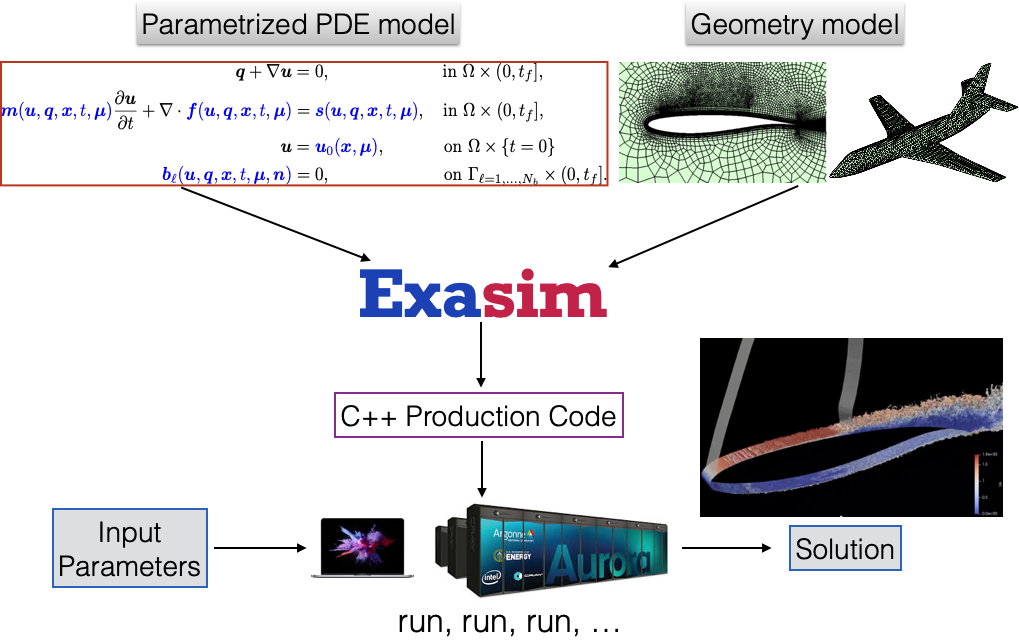
\includegraphics[scale=1.1]{exasim3.png} \\
%\caption{Exasim}
\label{fig1}
\end{center}
Figure 1:   A parametrized PDE model is input into  \texttt{Exasim} as functions (written in blue colors) of the field variables, spatial coordinates, time, and physical parameters.  A geometry model or a finite element mesh is needed to describe the physical domain.  \texttt{Exasim} generates C++ code to solve the parametrized PDE model for many input parameters across different computing platforms. 
\end{figure}

% While most computers have C++ compiler, {\tt sudo apt install gcc} on Linux and {\em brew install gcc} on Mac you may want to install newer version g++ ,  \href{https://developer.nvidia.com/cuda-toolkit}{CUDA Tookit} to download  and install it. sudo apt install libblas-dev liblapack-dev brew install openblas brew install lapack

What make \texttt{Exasim} unique are the following distinctive features: 

\begin{itemize}
\item \texttt{Exasim} intuitively simplifies  modeling and simulation % with an intuitive interface.
\item  generates stand-alone C++ production code and gives practitioners  freedom to modify the code and execute it as desired
\item provides implicit high-order DG solution of parametrized PDE models
\item provides full GPU functionality, meaning that all code components from discretization schemes to iterative solvers are deployed fully on GPUs
\item and is available in Julia, Python, and Matlab. 
\end{itemize}

\subsection{Obtaining Exasim}

Click \href{https://github.com/exapde/exasim}{here} to download \texttt{Exasim}'s  source code.  Alternatively, you can clone the repository directly on the command line via 

\hspace{5ex}  git clone https://github.com/exapde/Exasim.git

\texttt{Exasim}  is freely available under the MIT License. Please see the \href{https://opensource.org/licenses/MIT}{license details} for terms and conditions. 

After downloading the source code, please make sure that the name of the folder is \PY{I+s}{Exasim}. If it has a different name, please rename it to \PY{I+s}{Exasim}.


\subsection{Installing External Packages}

%\href{https://software.intel.com/content/www/us/en/develop/tools/math-kernel-library/choose-download.html}{MKL Intel library} is recommended if Blas/Lapack libraries are not yet installed on your computer. We recommend \href{https://www.ibm.com/products/spectrum-mpi}{IBM Spectrum MPI} for building memory-distributed applications on NVIDIA GPU clusters. 

\texttt{Exasim} automatically generates and compiles stand-alone C++ code on the fly. To do that, \texttt{Exasim} requires a C++ compiler and Blas/Lapack libraries to generate serial codes. An MPI library such as \href{https://www.open-mpi.org/}{Open-MPI} is required to generate parallel codes. \href{https://developer.nvidia.com/cuda-toolkit}{CUDA Tookit} is required to generate CUDA codes on Nvidia GPUs.  \href{http://gmsh.info/} {Gmsh} is used for mesh generation. \href{http://glaros.dtc.umn.edu/gkhome/metis/metis/overview}{METIS} is needed for mesh partition.  And \href{https://www.paraview.org/}{Paraview} is needed for visualization.

% The minimum requirements are a C++ compiler, Blas/Lapack libraries, and one of Julia, Python, or Matlab.

To install the required packages, please open Julia, Python, or Matlab and go to the folder \PY{I+s}{Exasim/Installation} and run the  \textcolor{orange}{install} script. 

If you use  \texttt{Exasim} with Julia, type the following line and hit return

\hspace{5ex} \PY{k}{julia>} include("install.jl")

If you use \texttt{Exasim} with Python, type the following line and hit return

\hspace{5ex} \PY{k}{> > >} exec(open("install.py").read())

If you use \texttt{Exasim} with Matlab, type the following line and hit return

\hspace{5ex} \PY{k}{> > } install

After installation, the executable files (or their symbolic links) of these packages are usually found in the directory \PY{I+s}{/usr/local/bin} or \PY{I+s}{/usr/bin}. To know the directory of an executable file, open the terminal and type ``which executable``. For example,  if you type ``which gmsh`` and see \PY{I+s}{/usr/local/bin/gmsh} or  \PY{I+s}{/usr/bin/gmsh} on the terminal screen, it means that Gmsh was installed  in the directory \PY{I+s}{/usr/local/bin} or \PY{I+s}{/usr/bin}, respectively. On the other hand, if you see  ``gmsh not found`` on the terminal screen, then either Gmsh is not installed or it is installed in a directory which is not included in the PATH environment variable. If Gmsh is not installed, you should install it. If Gmsh was already installed and you know the directory containing Gmsh's executable file, you must add that directory to the PATH environment variable. Please see the  \textcolor{orange}{setpath}  script  in the the folder \PY{I+s}{Exasim/Installation} for adding directories to the PATH environment variable. Doing so will enable \texttt{Exasim} to find the external softwares and run them. For example, when Paraview is installed on MacOS systems, it is usually installed in the directory \PY{I+s}{/Applications}. So, when you type ``which paraview`` in the terminal, you may see ``paraview not found`` even though it is already installed. This is because Paraview's executable file is located at the directory \PY{I+s}{/Applications/ParaView-5.8.1.app/Contents/MacOS} which is not included on the PATH environment variable. In order for \texttt{Exasim} to find paraview, you must include \PY{I+s}{/Applications/ParaView-5.8.1.app/Contents/MacOS} in the PATH environment variable. To do that, please modify the  \textcolor{orange}{setpath} script  in the the folder \PY{I+s}{Exasim/Installation}.

% /Applications/ParaView-5.8.1.app/Contents/MacOS/paraview

You can try \texttt{Exasim} without installing the required packages since \texttt{Exasim} automatically  searches the required packages on your computer system. If \texttt{Exasim}  could not find any required package, then follow the below steps to install that package.  

%Although \texttt{Exasim} will check the availability of these prerequisites on your computer, it is recommended to install them (at least, a C++ compiler and Blas/Lapack libraries) before using  \texttt{Exasim}. %We recommend practitioners to use the package manager \href{https://brew.sh/}{Homebrew} for the installation of software on macOS, Linux, and Windows Subsystem for Linux. Click \href{http://glaros.dtc.umn.edu/gkhome/metis/metis/overview}{here} to download and install METIS. After installation, METIS executable and library files must be placed in the folder \PY{I+s}{Exasim/metis/linux} for Linux computers, \PY{I+s}{Exasim/metis/mac} for Mac computers, or \PY{I+s}{Exasim/metis/windows} for Windows computers. 

\textbf{MacOS systems:} Most required external packages can be conveniently installed by using the package manager \href{https://brew.sh/}{Homebrew}. After installing \href{https://brew.sh/}{Homebrew},  open the terminal and run the following commands:

\hspace{5ex} \PY{k}{\$ } brew install gcc

\hspace{5ex} \PY{k}{\$ } brew install openblas

\hspace{5ex} \PY{k}{\$ } brew install lapack

\hspace{5ex} \PY{k}{\$ } brew install openmpi

\hspace{5ex} \PY{k}{\$ } brew install metis

\hspace{5ex} \PY{k}{\$ }  brew install gmsh

%\hspace{5ex} \PY{k}{\$ } ruby -e "\$(curl -fsSL https://raw.githubusercontent.com/Homebrew/install/master/install)" < /dev/null 2> /dev/null ; brew install caskroom/cask/brew-cask 2> /dev/null

\hspace{5ex} \PY{k}{\$ } brew cask install paraview

\hspace{5ex} \PY{k}{\$ } brew cask install julia

\hspace{5ex} \PY{k}{\$ } brew install python

%Before running these commands, please use "which"  command to check if some of these packages were already installed.

\textbf{Linux systems:} Open the terminal and run the following commands:

\hspace{5ex} \PY{k}{\$ } sudo apt install gcc

\hspace{5ex} \PY{k}{\$ } sudo apt install libblas-dev liblapack-dev

\hspace{5ex} \PY{k}{\$ } sudo apt install openmpi

\hspace{5ex} \PY{k}{\$ } sudo apt install metis

\hspace{5ex} \PY{k}{\$ } sudo apt install gmsh

\hspace{5ex} \PY{k}{\$ } sudo apt install paraview

\hspace{5ex} \PY{k}{\$ } sudo apt install julia

\hspace{5ex} \PY{k}{\$ } sudo apt install python

\textbf{Windows systems:} It is highly recommended to install the above packages via Windows Subsystem for Linux and Ubuntu. The installation on Windows Subsystem for Linux is the same as on Linux system.

As \texttt{Exasim} uses high-level languages to generate C++ code, you need one of the three languages Julia, Python, or Matlab to run \texttt{Exasim}. You can install Julia and Python as described above. Alternatively, wou can download and install \href{https://julialang.org/downloads/}{Julia} at the website \href{https://julialang.org/downloads/}{https://julialang.org/downloads/}. Optionally, we recommend you to install \href{https://atom.io/}{Atom editor}. Atom allows you to write C, C++, Julia, Python, Matlab codes and run your codes interactively.

%Julia  can be installed as follows
%\hspace{5ex} \PY{k}{\$ } brew cask install julia
%
%for MacOS systems,  and 
%
%\hspace{5ex} \PY{k}{\$ } sudo apt install julia

%for Linux systems. Alternatively, you can download and install \href{https://julialang.org/downloads/}{Julia} at the website \href{https://julialang.org/downloads/}{https://julialang.org/downloads/}. Optionally, we recommend \href{https://atom.io/}{Atom editor} for using Julia. Atom allows you to write C, C++, Julia, Python, Matlab codes and run your codes interactively.

Depending on which language you use to run \texttt{Exasim}, you need to install a few more packages.

\textbf{Julia:}    \texttt{Exasim}  requires  \href{https://github.com/JuliaPy/SymPy.jl}{ SymPy} and \href{https://timholy.github.io/Revise.jl/stable/}{Revise}, which can be obtained by using the following commands in Julia's REPL session 

\hspace{5ex} \PY{k}{julia>}  import Pkg; Pkg.add("SymPy"); Pkg.add("Revise");

It is important to note that Julia's SymPy calls Python's SymPy from Julia.  In order for Julia's SymPy to work., you need to install both Python and Python's SymPy. 
% Python can be installed as follows 
%
%\hspace{5ex} \PY{k}{\$ } brew install python
%
%for MacOS systems, and
%
%\hspace{5ex} \PY{k}{\$ } sudo apt install python
%
%for Linux systems.

\textbf{Python:} \texttt{Exasim} requires \href{https://www.scipy.org/install.html}{numpy, scipy, and sympy}, which can be obtained by using the following commands in the terminal 

\hspace{5ex} \PY{k}{\$ } sudo pip3 install numpy

\hspace{5ex} \PY{k}{\$ } sudo pip3 install scipy

\hspace{5ex} \PY{k}{\$ } sudo pip3 install sympy

for all operating systems.

\textbf{Matlab:}  \texttt{Exasim}  requires Symbolic Math Toolbox. 


\subsection{Examples}


Many examples are provided to illustrate how to generate DG codes for solving a wide variety of PDEs including Poisson equation, wave equation, heat equation, advection, convection-diffusion, elasticity, Euler equations, Navier-Stokes equations, and MHD equations. To try out any of the provided examples, practitioners go to a folder under \PY{I+s}{Exasim/Applications}  and run \textcolor{orange}{pdeapp.jl} in Julia REPL session, \textcolor{orange}{pdeapp.py} in Python REPL session, or \textcolor{orange}{pdeapp.m} in Matlab Command Window. 

%The folder \PY{I+s}{Exasim/Applications} contain many examples that illustrate how to use \texttt{Exasim} to build applications for solving PDEs. Inside every folder under \PY{I+s}{Exasim/Applications}, there are three script files: \textcolor{orange}{pdeapp.jl} for Julia, \textcolor{orange}{pdeapp.py} for Python, and \textcolor{orange}{pdeapp.m} for Matlab. Each script defines a particular PDE model, discretization parameters, solver parameters, compiler options, and produces input files. Then it generates C++/CUDA source code and compiles source code into an executable application. Finally, it runs the executable application to compute, store,  and visualize the numerical solution. 

For Julia, go to any folder under \PY{I+s}{Exasim/Applications}, type the following line and hit return

\hspace{5ex} \PY{k}{julia>} include("pdeapp.jl")

For Python, go to any folder under \PY{I+s}{Exasim/Applications}, type the following line and hit return

\hspace{5ex} \PY{k}{> > >} exec(open("pdeapp.py").read())

For Matlab, go to any folder under \PY{I+s}{Exasim/Applications}, type the following line and hit return

\hspace{5ex} \PY{k}{> > } pdeapp

If successful, \texttt{Exasim} produces three new folders. The \PY{I+s}{app} folder contains the source code and executable application, the \PY{I+s}{datain} folder contains input files for the executable application, and the \PY{I+s}{dataout} folder contains the output files produced by running the executable application,  which stores the numerical solution of the PDE model defined in the \textcolor{orange}{pdeapp} script.  \texttt{Exasim} also opens Paraview to visualize the numerical solution. Because \texttt{Exasim} runs the executable application in the REPL session, the executable prints out the simulation progress in the REPL session window. Alternatively, you can run the executable from the terminal. The generated source code can also be transferred to another computer and compiled to run on that computer.

New PDE models/DG solvers can be generated by making use of the provided examples. The process of generating DG code for a particular PDE model is described Section 4. 


% Practitioners may want to make use of these examples to build new applications. 

\subsection{PDE Models}

\texttt{Exasim} supports a wide range of PDE models described in Section \ref{PDEmodels}. Physical problems governed by these PDE models can be found in fluid mechanics, solid mechanics, and electromagnetism. 


\subsection{Finite Element Mesh}

 % A conformal linear finite element mesh is composed of $p$ and $t$, where $p \in \mathbb{R}^{n_d \times n_p}$ is a two-dimensional float array storing mesh points and $t \in \mathbb{R}^{n_v \times n_e}$  is a two-dimensional integer array storing mesh elements. 
 %A finite element mesh of a PDE model is a tessellation of its physical domain by simple geometrical elements of various shapes including triangles, quadrangles, tetrahedra, and hexahedra.
 
 \texttt{Exasim} provides a Mesh module to generate meshes for simple geometries. Any open-source mesh generators such as \href{https://cubit.sandia.gov/}{CUBIT}, \href{https://www.cgal.org/index.html}{CGAL}, \href{http://persson.berkeley.edu/distmesh/}{DistMesh},  \href{http://wias-berlin.de/software/index.jsp?id=TetGen&lang=1}{TetGen}, \href{https://www.mmgtools.org/}{Mmg}, \href{http://gmsh.info/} {Gmsh}, \href{https://www.meshlab.net/}{MeshLab}, \href{https://www.salome-platform.org/}{SALOME} can be used for complex geometries.   \texttt{Exasim} uses Gmsh to generate meshes from geometry model files. Because a high-order mesh is needed for the DG discretization of a PDE model, \texttt{Exasim} produces the high-order mesh from a standard finite element mesh. 

%Gmsh executable file must be placed in the folder \PY{I+s}{Exasim/gmsh/linux} for Linux computers, \PY{I+s}{Exasim/gmsh/mac} for Mac computers, or \PY{I+s}{Exasim/gmsh/windows} for Windows computers. 

\subsection{Discretization Methods}

Discretization methods refer to numerical methods used to discretize spatial derivatives and time derivatives of a PDE model. Discontinuous Galerkin (DG) methods are used for spatial discretization, while diagonally implicit Runge-kutta (DIRK) schemes are used for temporal discretization. These methods are implemented in C++ and the source codes can be found in the folder \PY{I+s}{Exasim/Version0.1/Kernel}. \texttt{Exasim} allows practitioners to implement a wide variety of DG methods (see Section 6 for details). 

\subsection{Matrix-Free Iterative Solvers}

Solvers refer to solution methods used to solve nonlinear and linear systems arising from the discretization of a PDE model. \texttt{Exasim} implements a matrix-free Newton-GMRES solver. Newton method is used to solve nonlinear systems of equations arising from the DG/DIRK discretization of PDE models. For each Newton iteration, GMRES is used to solve the resulting linear systems of equations. The matrix-vector multiplications in GMRES are computed in matrix-free fashion using Taylor's series expansion of the residual vector to the first order or the second order. Reduced basis method is used to construct an approximation to the Jacobian matrix for preconditioning the linear systems. The C++ implementation of these methods can be found in the folder \PY{I+s}{Exasim/Version0.1/Kernel}. 


\subsection{Visualization}

\texttt{Exasim} uses \href{https://www.paraview.org/}{Paraview} to visualize and analyze simulation results obtained by running the C++ production code. To do that, \texttt{Exasim}  generates VTU files and opens  \href{https://www.paraview.org/}{Paraview}  to visualize the computed solution. 

\subsection{Reporting Issues and Suggesting Improvements}

Please click \href{https://github.com/exapde/Exasim/issues}{here} to report any issues you encounter using \texttt{Exasim} and provide a detailed description of the issue as you can. If you have ideas for improvement, we would love to hear them by emailing us at exapde@gmail.com.

\section{Parametrized PDE Models}
\label{PDEmodels}

\texttt{Exasim} produces executable applications to solve a wide variety of PDE models. The underlying PDE system must be written as a set of first-order PDEs. In this section, we describe how to input a PDE model into \texttt{Exasim}. 


\subsection{Model C: Convection Model}

The Model C consists of any set of PDEs that can be written in the following form:
\begin{equation}
\label{modelc}
\bm m(\bm{u},\bm x,t, \bm \mu) \frac{\partial \bm{u}}{\partial t} + \nabla \cdot \bm{f}(\bm{u},\bm x,t, \bm \mu) = \bm s(\bm{u},\bm x,t, \bm \mu), \quad \mbox{in } \Omega \times (0, t_f], 
\end{equation}
with appropriate initial and boundary conditions. Here $\bm u = [u_1, u_2, \ldots, u_{n_{cu}}]$ is the vector of $n_{cu}$ state variables, $\bm x = [x_1,\dots,x_{n_d}]$ is the vector of coordinate variables in $\Omega$, $t$ represents time variable in $(0, t_f]$, and $\bm \mu = [\mu_1, \ldots, \mu_{n_{param}}]$ is a vector of $n_{param}$ physical parameters. The state vector $\bm u$ is the exact solution of the Model C (\ref{modelc}).  \texttt{Exasim} produces codes to compute the approximate solution $\bm u_h$.

The vector-valued function  $\bm m = [m_i(\bm u, \bm x, t, \bm \mu), 1 \le i \le n_{cu} ]$ is called {\em mass} function, the matrix-valued function $\bm f = [f_{ij}(\bm u, \bm x, t, \bm \mu), 1 \le i \le n_{cu}, 1 \le j \le n_d]$ is called {\em flux} function, The vector-valued function  $\bm s = [s_i(\bm u, \bm x, t, \bm \mu), 1 \le i \le n_{cu} ]$ is called {\em source} function. These functions are specified by writing functions in high-level languages (Julia, Python, or Matlab).

Examples of the Model C include linear convection equation, the Burgers equation, the Euler equations, and the shallow water equations. \texttt{Exasim} can solve both steady-state and unsteady problems. The steady-state version of the Model C can be obtained by setting $\bm m$ to zeros. 

\subsection{Model D: Convection-Diffusion Model}

The Model D consists of any set of PDEs that can be written in the following form:
\begin{equation}
\label{modeld0}
\bm m(\bm{u}, - \nabla \bm u, \bm x,t, \bm \mu) \frac{\partial \bm{u}}{\partial t} + \nabla \cdot \bm{f}(\bm{u}, - \nabla \bm u, \bm x,t, \bm \mu) = \bm s(\bm{u}, - \nabla \bm u, \bm x,t, \bm \mu), \quad \mbox{in } \Omega \times (0, t_f], 
\end{equation}
with appropriate initial and boundary conditions. The Model D is a generalization of the Model C by including the negative gradient of the state vector (i.e. $- \nabla \bm u$) in the {\em mass}, {\em flux}, and {\em source} functions.

It is convenient to introduce additional state variables $\bm q = - \nabla \bm u$  and rewrite the Model D as follows
\begin{subequations}
\label{modeld}
\begin{alignat}{2}
\bm q + \nabla \bm u & =  \bm 0,  & \quad \mbox{in } \Omega \times (0, t_f], \\
\bm m(\bm{u}, \bm q, \bm x,t, \bm \mu) \frac{\partial \bm{u}}{\partial t} + \nabla \cdot \bm{f}(\bm{u}, \bm q, \bm x,t, \bm \mu) &=  \bm s(\bm{u}, \bm q, \bm x,t, \bm \mu), & \quad \mbox{in } \Omega \times (0, t_f], 
\end{alignat}
\end{subequations}
with appropriate initial and boundary conditions. The set of state variables $(\bm u, \bm q)$ is the exact solution of the Model D (\ref{modeld}). \texttt{Exasim} produces codes to compute the approximate solution $(\bm u_h, \bm q_h)$.

%\begin{equation*}
%\begin{split}
%\bm q + \nabla \bm u & = 0, \hspace{2.3cm} \mbox{in } \Omega \times (0, t_f], \\
%\bm m(\bm{u}, \bm q, \bm x,t, \bm \mu) \frac{\partial \bm{u}}{\partial t} + \nabla \cdot \bm{f}(\bm{u}, \bm q, \bm x,t, \bm \mu) & = \bm s(\bm{u}, \bm q, \bm x,t, \bm \mu), \quad \mbox{in } \Omega \times (0, t_f], \\
%\bm u & = \bm u_0(\bm x, \bm \mu), \hspace{1.2cm} \mbox{on } \Omega \times \{t=0\} \\
%\bm b_\ell(\bm u, \bm q, \bm x, t, \bm \mu, \bm n) & = 0, \hspace{2.33cm} \mbox{on } \Gamma_\ell  \times (0, t_f], \ \ell = 1, \ldots, N_b 
%\end{split}
%\end{equation*}

Examples of the Model D include the Poisson equation, convection-diffusion equations, linear elasticity equations, nonlinear elasticity equations, the incompressible Navier-Stokes equations, and the compressible Navier-Stokes equations. 

\subsection{Model W: Wave Model}

The Model W consists of any set of PDEs that can be written in the following form:
\begin{equation}
\label{modelw0}
\bm m \left(\frac{\partial \bm{w}}{\partial t}, - \nabla \bm w, \bm x,t, \bm \mu\right) \frac{\partial^2 \bm{w}}{\partial t^2}  + \nabla \cdot \bm{f} \left(\frac{\partial \bm{w}}{\partial t}, - \nabla \bm w, \bm x,t, \bm \mu\right) = \bm s \left(\frac{\partial \bm{w}}{\partial t}, - \nabla \bm w, \bm x,t, \bm \mu\right), 
\end{equation}
with appropriate initial and boundary conditions. The Model W is a generalization of the Model D by having the second-order time derivatives.


It is convenient to introduce additional state variables $\bm u = \frac{\partial \bm{w}}{\partial t}$,  $\bm q = - \nabla \bm w$,  and rewrite the Model D as follows
\begin{subequations}
\label{modelw}
\begin{alignat}{2}
\frac{\partial \bm w}{\partial t} - \bm u & =  \bm 0,  & \quad \mbox{in } \Omega \times (0, t_f], \\
\frac{\partial \bm q}{\partial t} + \nabla \bm u & =  \bm 0,  & \quad \mbox{in } \Omega \times (0, t_f], \\
\bm m(\bm{u}, \bm q,  \bm x,t, \bm \mu) \frac{\partial \bm{u}}{\partial t} + \nabla \cdot \bm{f}(\bm{u}, \bm q, \bm x,t, \bm \mu) &=  \bm s(\bm{u}, \bm q,   \bm x,t, \bm \mu), & \quad \mbox{in } \Omega \times (0, t_f].  
\end{alignat}
\end{subequations}
The set of state variables $(\bm u, \bm q, \bm w)$ is the exact solution of the Model W (\ref{modelw}). \texttt{Exasim} produces codes to compute the approximate solution $(\bm u_h, \bm q_h, \bm w_h)$.


The Model W deals with wave propagation problems.  Examples of the Model D include the wave equation, linear elastodynamics, nonlinear elastodynamics, and the Maxwell's equations. 

%\subsection{Model A: Algebraic-Differential Model}
%
%
%%It is convenient to introduce additional state variables $\bm u = \frac{\partial \bm{w}}{\partial t}$,  $\bm q = - \nabla \bm w$,  and rewrite the Model D as follows
%\begin{subequations}
%\label{modela}
%\begin{alignat}{2}
%\bm q + \nabla \bm u & =  \bm 0,  & \quad \mbox{in } \Omega \times (0, t_f], \\
%\bm m(\bm{u}, \bm q,  \bm w, \bm x,t, \bm \mu) \frac{\partial \bm{u}}{\partial t} + \nabla \cdot \bm{f}(\bm{u}, \bm q, \bm w, \bm x,t, \bm \mu) &=  \bm s(\bm{u}, \bm q, \bm w,  \bm x,t, \bm \mu), & \quad \mbox{in } \Omega \times (0, t_f], \\
%\bm m_w \frac{\partial \bm w}{\partial t}   +  \bm w & =  \bm s_w(\bm u, \bm q, x, t, \bm \mu),  & \quad \mbox{in } \Omega \times (0, t_f] .
%\end{alignat}
%\end{subequations}
%The set of state variables $(\bm u, \bm q, \bm w)$ is the exact solution of the Model W (\ref{modelw}). \texttt{Exasim} produces codes to compute the approximate solution $(\bm u_h, \bm q_h, \bm w_h)$.
%
%
%The Model W deals with wave propagation problems.  Examples of the Model D include the wave equation, linear elastodynamics, nonlinear elastodynamics, and the Maxwell's equations. 


\subsection{High-Order PDE Models}

Elliptic, parabolic, and hyperbolic PDEs of order two are widely used to model physical problems in engineering and science. However, there many other important types of PDE, including the Korteweg-de Vries (KdV) equation and the biharmonic equation.  We will show that \texttt{Exasim} can deal with high-order PDEs. To this end, we consider the fourth-order biharmonic equation
\begin{equation}
\Delta^2 u = f(\bm x) ,
\end{equation}
with appropriate boundary conditions. We introduce a new variable $v = - \Delta u$ and write the fourth-order biharmonic equation as a set of two coupled Poisson equations as follows 
\begin{subequations}
\begin{alignat}{2}
-\Delta v & = f,\\
-\Delta u & = v .
\end{alignat}
\end{subequations}
We next define $\bm u = [v, u]$, $\bm s = [f, v]$, $\bm q = - \nabla \bm u$, and rewrite the above system as follows
\begin{subequations}
\begin{alignat}{2}
\bm q + \nabla \bm u & = 0,\\
\nabla \cdot \bm q & = \bm s(\bm u, \bm x) .
\end{alignat}
\end{subequations}
This set of PDEs belongs to the Model D (\ref{modeld}).

In general, high-order PDEs can be written as a set of first-order PDEs by introducing new state variables. Indeed, the Model C (\ref{modelc}), Model D (\ref{modeld}), and Model W (\ref{modelw}) are nothing but a set of first-order PDEs. 

\subsection{PDE Model File}

Practitioners write a PDE model file to define a parametrized PDE model to be solved.  This involves writing  {\em mass}, {\em flux},  {\em source}, {\em ubou},  {\em fbou},  {\em initu}, {\em initq}, {\em initw}, and {\em initv} functions in terms of the state variables $(\bm u, \bm q, \bm w)$, spatial variables $\bm x$, time variable $t$, and physical parameters $\bm \mu$, to define governing equations and boundary conditions. We extend these functions with two new variables, $\bm v$ and $\bm \eta$, which represent the external fields and external parameters, respectively. This extension allows a mean to coupling \texttt{Exasim} with an external code through the external fields $\bm v$ and external parameters $\bm \eta$. 

\begin{itemize}
\item The first three functions,  {\em mass},  {\em flux}, and  {\em source},  implement the mass $\bm m$, flux $\bm f$, and source $\bm s$, respectively. 

\item The next two functions,  {\em ubou}, and {\em fbou}, implement the boundary values for the solution $\bm u$ and the normal component of the flux $\bm f_b = \bm f \cdot \bm n$, respectively. Both  {\em ubou}, and {\em fbou} also depends on the trace variables $\widehat{\bm{u}}$, the normal vector $\bm n$, and the DG stabilization parameter $\tau$ (see Section 6 for details.) 

\item The last four functions, {\em initu}, {\em initq}, {\em initw}, and {\em initv}, implement the initial values for $\bm u$, $\bm q$, $\bm w$, and $\bm v$, respectively. 
\end{itemize}

Below is a "blank" PDE model file which does not define these functions yet. It gives a sense of how these functions should be defined. Depending on a particular PDE model, you need to define these functions accordingly. 

    \begin{tcolorbox}[breakable, size=fbox, boxrule=1pt, pad at break*=1mm,colback=cellbackground, colframe=cellborder]
\begin{Verbatim}[commandchars=\\\{\}]
\PY{k}{function} \PY{n}{mass}\PY{p}{(}\PY{n}{u}\PY{p}{,} \PY{n}{q}\PY{p}{,} \PY{n}{w}\PY{p}{,} \PY{n}{v}\PY{p}{,} \PY{n}{x}\PY{p}{,} \PY{n}{t}\PY{p}{,} \PY{n}{mu}\PY{p}{,} \PY{n}{eta}\PY{p}{)}
    \PY{c}{\PYZsh{} define m below}
    \PY{k}{return} \PY{n}{m}\PY{p}{;}
\PY{k}{end}
\PY{k}{function} \PY{n}{flux}\PY{p}{(}\PY{n}{u}\PY{p}{,} \PY{n}{q}\PY{p}{,} \PY{n}{w}\PY{p}{,} \PY{n}{v}\PY{p}{,} \PY{n}{x}\PY{p}{,} \PY{n}{t}\PY{p}{,} \PY{n}{mu}\PY{p}{,} \PY{n}{eta}\PY{p}{)}
    \PY{c}{\PYZsh{} define f below}
    \PY{k}{return} \PY{n}{f}\PY{p}{;}
\PY{k}{end}
\PY{k}{function} \PY{n}{source}\PY{p}{(}\PY{n}{u}\PY{p}{,} \PY{n}{q}\PY{p}{,} \PY{n}{w}\PY{p}{,} \PY{n}{v}\PY{p}{,} \PY{n}{x}\PY{p}{,} \PY{n}{t}\PY{p}{,} \PY{n}{mu}\PY{p}{,} \PY{n}{eta}\PY{p}{)}
    \PY{c}{\PYZsh{} define s below }
    \PY{k}{return} \PY{n}{s}\PY{p}{;}
\PY{k}{end}
\PY{k}{function} \PY{n}{ubou}\PY{p}{(}\PY{n}{u}\PY{p}{,} \PY{n}{q}\PY{p}{,} \PY{n}{w}\PY{p}{,} \PY{n}{v}\PY{p}{,} \PY{n}{x}\PY{p}{,} \PY{n}{t}\PY{p}{,} \PY{n}{mu}\PY{p}{,} \PY{n}{eta}\PY{p}{,} \PY{n}{uhat}\PY{p}{,} \PY{n}{n}\PY{p}{,} \PY{n}{tau}\PY{p}{)}
    \PY{c}{\PYZsh{} define ub below }
    \PY{k}{return} \PY{n}{ub}\PY{p}{;}
\PY{k}{end}
\PY{k}{function} \PY{n}{fbou}\PY{p}{(}\PY{n}{u}\PY{p}{,} \PY{n}{q}\PY{p}{,} \PY{n}{w}\PY{p}{,} \PY{n}{v}\PY{p}{,} \PY{n}{x}\PY{p}{,} \PY{n}{t}\PY{p}{,} \PY{n}{mu}\PY{p}{,} \PY{n}{eta}\PY{p}{,} \PY{n}{uhat}\PY{p}{,} \PY{n}{n}\PY{p}{,} \PY{n}{tau}\PY{p}{)}
    \PY{c}{\PYZsh{} define fb below }
    \PY{k}{return} \PY{n}{fb}\PY{p}{;}
\PY{k}{end}
\PY{k}{function} \PY{n}{initu}\PY{p}{(}\PY{n}{x}\PY{p}{,} \PY{n}{mu}\PY{p}{,} \PY{n}{eta}\PY{p}{)}
    \PY{c}{\PYZsh{} define u0 below }
    \PY{k}{return} \PY{n}{u0}\PY{p}{;}
\PY{k}{end}
\PY{k}{function} \PY{n}{initq}\PY{p}{(}\PY{n}{x}\PY{p}{,} \PY{n}{mu}\PY{p}{,} \PY{n}{eta}\PY{p}{)}
    \PY{c}{\PYZsh{} define q0 below }
    \PY{k}{return} \PY{n}{q0}\PY{p}{;}
\PY{k}{end}
\PY{k}{function} \PY{n}{initw}\PY{p}{(}\PY{n}{x}\PY{p}{,} \PY{n}{mu}\PY{p}{,} \PY{n}{eta}\PY{p}{)}
    \PY{c}{\PYZsh{} define w0 below }
    \PY{k}{return} \PY{n}{w0}\PY{p}{;}
\PY{k}{end}
\PY{k}{function} \PY{n}{initv}\PY{p}{(}\PY{n}{x}\PY{p}{,} \PY{n}{mu}\PY{p}{,} \PY{n}{eta}\PY{p}{)}
    \PY{c}{\PYZsh{} define v0 below }
    \PY{k}{return} \PY{n}{v0}\PY{p}{;}
\PY{k}{end}
\end{Verbatim}
\end{tcolorbox}

 
Let's consider the Poisson equation $-\nabla \cdot \mu_1 \nabla u = 3 \pi^2 \sin(\pi x_1) \sin(\pi x_2) \sin(\pi x_3)$ rewritten as
\begin{equation}
\label{poi3d}
\nabla \cdot \mu_1 \bm q = 3 \pi^2 \sin(\pi x_1) \sin(\pi x_2) \sin(\pi x_3), \qquad \bm q + \nabla u = 0, 
\end{equation}
in a physical domain $\Omega$ with $u = \mu_2$ on $\partial \Omega$. The PDE model file for the above Poisson equation is listed below

    \begin{tcolorbox}[breakable, size=fbox, boxrule=1pt, pad at break*=1mm,colback=cellbackground, colframe=cellborder]
\begin{Verbatim}[commandchars=\\\{\}]
\PY{k}{function} \PY{n}{flux}\PY{p}{(}\PY{n}{u}\PY{p}{,} \PY{n}{q}\PY{p}{,} \PY{n}{w}\PY{p}{,} \PY{n}{v}\PY{p}{,} \PY{n}{x}\PY{p}{,} \PY{n}{t}\PY{p}{,} \PY{n}{mu}\PY{p}{,} \PY{n}{eta}\PY{p}{)}
    \PY{n}{f} \PY{o}{=} \PY{n}{mu}\PY{p}{[}\PY{l+m+mi}{1}\PY{p}{]}\PY{o}{*}\PY{n}{q}\PY{p}{;}
    \PY{k}{return} \PY{n}{f}\PY{p}{;}
\PY{k}{end}
\PY{k}{function} \PY{n}{source}\PY{p}{(}\PY{n}{u}\PY{p}{,} \PY{n}{q}\PY{p}{,} \PY{n}{w}\PY{p}{,} \PY{n}{v}\PY{p}{,} \PY{n}{x}\PY{p}{,} \PY{n}{t}\PY{p}{,} \PY{n}{mu}\PY{p}{,} \PY{n}{eta}\PY{p}{)}
    \PY{n}{s} \PY{o}{=} \PY{p}{(}\PY{l+m+mi}{3}\PY{o}{*}\PY{n+nb}{pi}\PY{o}{*}\PY{n+nb}{pi}\PY{p}{)}\PY{o}{*}\PY{n}{sin}\PY{p}{(}\PY{n+nb}{pi}\PY{o}{*}\PY{n}{x}\PY{p}{[}\PY{l+m+mi}{1}\PY{p}{]}\PY{p}{)}\PY{o}{*}\PY{n}{sin}\PY{p}{(}\PY{n+nb}{pi}\PY{o}{*}\PY{n}{x}\PY{p}{[}\PY{l+m+mi}{2}\PY{p}{]}\PY{p}{)}\PY{o}{*}\PY{n}{sin}\PY{p}{(}\PY{n+nb}{pi}\PY{o}{*}\PY{n}{x}\PY{p}{[}\PY{l+m+mi}{3}\PY{p}{]}\PY{p}{)}\PY{p}{;}
    \PY{k}{return} \PY{n}{s}\PY{p}{;}
\PY{k}{end}
\PY{k}{function} \PY{n}{ubou}\PY{p}{(}\PY{n}{u}\PY{p}{,} \PY{n}{q}\PY{p}{,} \PY{n}{w}\PY{p}{,} \PY{n}{v}\PY{p}{,} \PY{n}{x}\PY{p}{,} \PY{n}{t}\PY{p}{,} \PY{n}{mu}\PY{p}{,} \PY{n}{eta}\PY{p}{,} \PY{n}{uhat}\PY{p}{,} \PY{n}{n}\PY{p}{,} \PY{n}{tau}\PY{p}{)}
    \PY{n}{ub} \PY{o}{=} \PY{n}{mu}\PY{p}{[}\PY{l+m+mi}{2}\PY{p}{]}\PY{p}{;}
    \PY{k}{return} \PY{n}{ub}\PY{p}{;}
\PY{k}{end}
\PY{k}{function} \PY{n}{fbou}\PY{p}{(}\PY{n}{u}\PY{p}{,} \PY{n}{q}\PY{p}{,} \PY{n}{w}\PY{p}{,} \PY{n}{v}\PY{p}{,} \PY{n}{x}\PY{p}{,} \PY{n}{t}\PY{p}{,} \PY{n}{mu}\PY{p}{,} \PY{n}{eta}\PY{p}{,} \PY{n}{uhat}\PY{p}{,} \PY{n}{n}\PY{p}{,} \PY{n}{tau}\PY{p}{)}
    \PY{n}{f} \PY{o}{=} \PY{n}{flux}\PY{p}{(}\PY{n}{u}\PY{p}{,} \PY{n}{q}\PY{p}{,} \PY{n}{w}\PY{p}{,} \PY{n}{v}\PY{p}{,} \PY{n}{x}\PY{p}{,} \PY{n}{t}\PY{p}{,} \PY{n}{mu}\PY{p}{,} \PY{n}{eta}\PY{p}{)}\PY{p}{;}
    \PY{n}{fb} \PY{o}{=} \PY{n}{f}\PY{p}{[}\PY{l+m+mi}{1}\PY{p}{]}\PY{o}{*}\PY{n}{n}\PY{p}{[}\PY{l+m+mi}{1}\PY{p}{]} \PY{o}{+} \PY{n}{f}\PY{p}{[}\PY{l+m+mi}{2}\PY{p}{]}\PY{o}{*}\PY{n}{n}\PY{p}{[}\PY{l+m+mi}{2}\PY{p}{]} \PY{o}{+} \PY{n}{f}\PY{p}{[}\PY{l+m+mi}{3}\PY{p}{]}\PY{o}{*}\PY{n}{n}\PY{p}{[}\PY{l+m+mi}{3}\PY{p}{]} \PY{o}{+} \PY{n}{tau}\PY{p}{[}\PY{l+m+mi}{1}\PY{p}{]}\PY{o}{*}\PY{p}{(}\PY{n}{u}\PY{p}{[}\PY{l+m+mi}{1}\PY{p}{]}\PY{o}{\PYZhy{}}\PY{n}{uhat[1]}\PY{p}{)}\PY{p}{;}
    \PY{k}{return} \PY{n}{fb}\PY{p}{;}
\PY{k}{end}
\PY{k}{function} \PY{n}{initu}\PY{p}{(}\PY{n}{x}\PY{p}{,} \PY{n}{mu}\PY{p}{,} \PY{n}{eta}\PY{p}{)}
    \PY{n}{u0} \PY{o}{=} \PY{l+m+mf}{0.0}\PY{p}{;}
    \PY{k}{return} \PY{n}{u0}\PY{p}{;}
\PY{k}{end}
\end{Verbatim}
\end{tcolorbox}


    \begin{tcolorbox}[breakable, size=fbox, boxrule=1pt, pad at break*=1mm,colback=cellbackground, colframe=cellborder]
\begin{Verbatim}[commandchars=\\\{\}]
\PY{k}{function} \PY{n}{f = flux}\PY{p}{(}\PY{n}{u}\PY{p}{,} \PY{n}{q}\PY{p}{,} \PY{n}{w}\PY{p}{,} \PY{n}{v}\PY{p}{,} \PY{n}{x}\PY{p}{,} \PY{n}{t}\PY{p}{,} \PY{n}{mu}\PY{p}{,} \PY{n}{eta}\PY{p}{)}
    \PY{n}{f} \PY{o}{=} \PY{n}{mu}\PY{p}{[}\PY{l+m+mi}{1}\PY{p}{]}\PY{o}{*}\PY{n}{q}\PY{p}{;}
\PY{k}{end}
\PY{k}{function} \PY{n}{s = source}\PY{p}{(}\PY{n}{u}\PY{p}{,} \PY{n}{q}\PY{p}{,} \PY{n}{w}\PY{p}{,} \PY{n}{v}\PY{p}{,} \PY{n}{x}\PY{p}{,} \PY{n}{t}\PY{p}{,} \PY{n}{mu}\PY{p}{,} \PY{n}{eta}\PY{p}{)}
    \PY{n}{s} \PY{o}{=} \PY{p}{(}\PY{l+m+mi}{3}\PY{o}{*}\PY{n+nb}{pi}\PY{o}{*}\PY{n+nb}{pi}\PY{p}{)}\PY{o}{*}\PY{n}{sin}\PY{p}{(}\PY{n+nb}{pi}\PY{o}{*}\PY{n}{x}\PY{p}{[}\PY{l+m+mi}{1}\PY{p}{]}\PY{p}{)}\PY{o}{*}\PY{n}{sin}\PY{p}{(}\PY{n+nb}{pi}\PY{o}{*}\PY{n}{x}\PY{p}{[}\PY{l+m+mi}{2}\PY{p}{]}\PY{p}{)}\PY{o}{*}\PY{n}{sin}\PY{p}{(}\PY{n+nb}{pi}\PY{o}{*}\PY{n}{x}\PY{p}{[}\PY{l+m+mi}{3}\PY{p}{]}\PY{p}{)}\PY{p}{;}
\PY{k}{end}
\PY{k}{function} \PY{n}{ub = ubou}\PY{p}{(}\PY{n}{u}\PY{p}{,} \PY{n}{q}\PY{p}{,} \PY{n}{w}\PY{p}{,} \PY{n}{v}\PY{p}{,} \PY{n}{x}\PY{p}{,} \PY{n}{t}\PY{p}{,} \PY{n}{mu}\PY{p}{,} \PY{n}{eta}\PY{p}{,} \PY{n}{uhat}\PY{p}{,} \PY{n}{n}\PY{p}{,} \PY{n}{tau}\PY{p}{)}
    \PY{n}{ub} \PY{o}{=} \PY{n}{mu}\PY{p}{[}\PY{l+m+mi}{2}\PY{p}{]}\PY{p}{;}
\PY{k}{end}
\PY{k}{function} \PY{n}{fb = fbou}\PY{p}{(}\PY{n}{u}\PY{p}{,} \PY{n}{q}\PY{p}{,} \PY{n}{w}\PY{p}{,} \PY{n}{v}\PY{p}{,} \PY{n}{x}\PY{p}{,} \PY{n}{t}\PY{p}{,} \PY{n}{mu}\PY{p}{,} \PY{n}{eta}\PY{p}{,} \PY{n}{uhat}\PY{p}{,} \PY{n}{n}\PY{p}{,} \PY{n}{tau}\PY{p}{)}
    \PY{n}{f} \PY{o}{=} \PY{n}{flux}\PY{p}{(}\PY{n}{u}\PY{p}{,} \PY{n}{q}\PY{p}{,} \PY{n}{w}\PY{p}{,} \PY{n}{v}\PY{p}{,} \PY{n}{x}\PY{p}{,} \PY{n}{t}\PY{p}{,} \PY{n}{mu}\PY{p}{,} \PY{n}{eta}\PY{p}{)}\PY{p}{;}
    \PY{n}{fb} \PY{o}{=} \PY{n}{f}\PY{p}{[}\PY{l+m+mi}{1}\PY{p}{]}\PY{o}{*}\PY{n}{n}\PY{p}{[}\PY{l+m+mi}{1}\PY{p}{]} \PY{o}{+} \PY{n}{f}\PY{p}{[}\PY{l+m+mi}{2}\PY{p}{]}\PY{o}{*}\PY{n}{n}\PY{p}{[}\PY{l+m+mi}{2}\PY{p}{]} \PY{o}{+} \PY{n}{f}\PY{p}{[}\PY{l+m+mi}{3}\PY{p}{]}\PY{o}{*}\PY{n}{n}\PY{p}{[}\PY{l+m+mi}{3}\PY{p}{]} \PY{o}{+} \PY{n}{tau}\PY{p}{[}\PY{l+m+mi}{1}\PY{p}{]}\PY{o}{*}\PY{p}{(}\PY{n}{u}\PY{p}{[}\PY{l+m+mi}{1}\PY{p}{]}\PY{o}{\PYZhy{}}\PY{n}{uhat[1]}\PY{p}{)}\PY{p}{;}
\PY{k}{end}
\PY{k}{function} \PY{n}{u0 = initu}\PY{p}{(}\PY{n}{x}\PY{p}{,} \PY{n}{mu}\PY{p}{,} \PY{n}{eta}\PY{p}{)}
    \PY{n}{u0} \PY{o}{=} \PY{l+m+mf}{0.0}\PY{p}{;}
\PY{k}{end}
\end{Verbatim}
\end{tcolorbox}

%\begin{verbatim}
%template <typename T> void cpuSource(T *s, T *xdg, T *udg, T *odg, T *wdg, T *uinf, 
%T *param, T time, int ng, int nc, int ncu, int nd, int ncx, int nco, int ncw)
%{
%	    #pragma omp parallel for
%	    for (int i = 0; i <ng; i++) {
%        			T xdg1 = xdg[0*ng+i];
%	        		T xdg2 = xdg[1*ng+i];
%        			T xdg3 = xdg[2*ng+i];
%        			s[0*ng+i] = sin(xdg1*3.141592653589793)*sin(xdg2*3.141592653589793)
%        		             *sin(xdg3*3.141592653589793)*2.960881320326807E1;
%	    }
%}
%template void cpuSource(double *, double *, double *, double *, double *, double *,
%     double *, double, int, int, int, int, int, int, int);
%template void cpuSource(float *, float *, float *, float *, float *, float *, 
%     float *, float, int, int, int, int, int, int, int);
%\end{verbatim}
%
%
%\begin{verbatim}
%template <typename T>  __global__  void kernelgpuFlux(T *f, T *xdg, T *udg, T *odg, 
%T *wdg, T *uinf, T *param, T time, int ng, int nc, int ncu, int nd, int ncx, int nco, int ncw)
%{
%	   int i = threadIdx.x + blockIdx.x * blockDim.x;
%	   while (i<ng) {
%		 	      T param1 = param[0];
%		   	    T udg2 = udg[1*ng+i];
%	   	    T udg3 = udg[2*ng+i];
%	  	     T udg4 = udg[3*ng+i];
%   	  	 f[0*ng+i] = param1*udg2;
%	  	     f[1*ng+i] = param1*udg3;
%	  	   f[2*ng+i] = param1*udg4;
%	  	i += blockDim.x * gridDim.x;
%	   }  
%}
%\end{verbatim}


Since this particular equation has zero mass function, i.e., $\bm m = 0$, we do not need to define the {\em mass} function in the PDE model file. This also applies to the {\em source} function, that is, if $\bm s = 0$, then we do not need to define the {\em source} function in the PDE model file. The initial guess for the solution $u$ of the Poisson equation is implemented in the function {\em initu}.

Instead of the Poisson equation if we would like to solve the following heat equation
\begin{equation}
\mu_3 \frac{\partial u}{\partial t}  + \nabla \cdot \mu_1 \bm q = 3 \pi^2 \sin(\pi x_1) \sin(\pi x_2) \sin(\pi x_3), \qquad \bm q + \nabla u = 0, 
\end{equation}
with the initial solution $u(\bm x, t=0) = 0$, then we need to add the following snippet to the above PDE model file
    \begin{tcolorbox}[breakable, size=fbox, boxrule=1pt, pad at break*=1mm,colback=cellbackground, colframe=cellborder]
\begin{Verbatim}[commandchars=\\\{\}]
\PY{k}{function} \PY{n}{mass}\PY{p}{(}\PY{n}{u}\PY{p}{,} \PY{n}{q}\PY{p}{,} \PY{n}{w}\PY{p}{,} \PY{n}{v}\PY{p}{,} \PY{n}{x}\PY{p}{,} \PY{n}{t}\PY{p}{,} \PY{n}{mu}\PY{p}{,} \PY{n}{eta}\PY{p}{)}
    \PY{n}{m} \PY{o}{=} \PY{n}{mu}\PY{p}{[}\PY{l+m+mi}{3}\PY{p}{]}\PY{p}{;}
    \PY{k}{return} \PY{n}{m}\PY{p}{;}
\PY{k}{end}
\end{Verbatim}
\end{tcolorbox}

Next, we assume that we want to solve the following 2D convection-diffusion equation
\begin{equation}
\mu_2 \frac{\partial u}{\partial t}  + \nabla \cdot (\mu_1 \bm q  + \bm c u) = 0, \qquad \bm q + \nabla u = 0, 
\end{equation}
with two boundary conditions $u = 0$ on $\Gamma_1$ and $(\mu_1 \bm q + c u) \cdot \bm n = -1$ on $\Gamma_2$ and the initial solution $u(\bm x, t=0) = \mu_3$. Here $\bm c =  (x_2, -x_1)$ is the convective velocity. The PDE model file for the above equation is listed below
 
    \begin{tcolorbox}[breakable, size=fbox, boxrule=1pt, pad at break*=1mm,colback=cellbackground, colframe=cellborder]
\begin{Verbatim}[commandchars=\\\{\}]
\PY{k}{function} \PY{n}{mass}\PY{p}{(}\PY{n}{u}\PY{p}{,} \PY{n}{q}\PY{p}{,} \PY{n}{w}\PY{p}{,} \PY{n}{v}\PY{p}{,} \PY{n}{x}\PY{p}{,} \PY{n}{t}\PY{p}{,} \PY{n}{mu}\PY{p}{,} \PY{n}{eta}\PY{p}{)}
    \PY{n}{m} \PY{o}{=} \PY{n}{mu}\PY{p}{[}\PY{l+m+mi}{2}\PY{p}{]}\PY{p}{;}
    \PY{k}{return} \PY{n}{m}\PY{p}{;}
\PY{k}{end}
\PY{k}{function} \PY{n}{flux}\PY{p}{(}\PY{n}{u}\PY{p}{,} \PY{n}{q}\PY{p}{,} \PY{n}{w}\PY{p}{,} \PY{n}{v}\PY{p}{,} \PY{n}{x}\PY{p}{,} \PY{n}{t}\PY{p}{,} \PY{n}{mu}\PY{p}{,} \PY{n}{eta}\PY{p}{)}
    \PY{n}{f} \PY{o}{=} \PY{l+m+mf}{0.0}\PY{o}{*}\PY{n}{q}\PY{p}{;}
    \PY{n}{f}\PY{p}{[}\PY{l+m+mi}{1}\PY{p}{]} \PY{o}{=} \PY{n}{mu}\PY{p}{[}\PY{l+m+mi}{1}\PY{p}{]}\PY{o}{*}\PY{n}{q}\PY{p}{[}\PY{l+m+mi}{1}\PY{p}{]} \PY{o}{+} \PY{n}{x}\PY{p}{[}\PY{l+m+mi}{2}\PY{p}{]}\PY{o}{*}\PY{n}{u}\PY{p}{[}\PY{l+m+mi}{1}\PY{p}{]}\PY{p}{;}
    \PY{n}{f}\PY{p}{[}\PY{l+m+mi}{2}\PY{p}{]} \PY{o}{=} \PY{n}{mu}\PY{p}{[}\PY{l+m+mi}{1}\PY{p}{]}\PY{o}{*}\PY{n}{q}\PY{p}{[}\PY{l+m+mi}{2}\PY{p}{]} \PY{o}{\PYZhy{}} \PY{n}{x}\PY{p}{[}\PY{l+m+mi}{1}\PY{p}{]}\PY{o}{*}\PY{n}{u}\PY{p}{[}\PY{l+m+mi}{1}\PY{p}{]}\PY{p}{;}    
    \PY{k}{return} \PY{n}{f}\PY{p}{;}
\PY{k}{end}
\PY{k}{function} \PY{n}{ubou}\PY{p}{(}\PY{n}{u}\PY{p}{,} \PY{n}{q}\PY{p}{,} \PY{n}{w}\PY{p}{,} \PY{n}{v}\PY{p}{,} \PY{n}{x}\PY{p}{,} \PY{n}{t}\PY{p}{,} \PY{n}{mu}\PY{p}{,} \PY{n}{eta}\PY{p}{,} \PY{n}{uhat}\PY{p}{,} \PY{n}{n}\PY{p}{,} \PY{n}{tau}\PY{p}{)}
    \PY{n}{ub} \PY{o}{=} \PY{p}{[}\PY{l+m+mi}{0}\PY{o}{*}\PY{n}{u}\PY{p}{[}\PY{l+m+mi}{1}\PY{p}{]}\PY{p}{,} \PY{l+m+mi}{0}\PY{o}{*}\PY{n}{u}\PY{p}{[}\PY{l+m+mi}{1}\PY{p}{]}\PY{p}{]}\PY{p}{;}
    \PY{n}{ub}\PY{p}{[}\PY{l+m+mi}{1}\PY{p}{]} \PY{o}{=} \PY{l+m+mi}{0}\PY{p}{;}     \PY{c}{\PYZsh{} Dirichlet boundary condition}
    \PY{n}{ub}\PY{p}{[}\PY{l+m+mi}{2}\PY{p}{]} \PY{o}{=} \PY{n}{u[1]}\PY{p}{;}  \PY{c}{\PYZsh{} Neumann boundary condition}
    \PY{k}{return} \PY{n}{ub}\PY{p}{;}
\PY{k}{end}
\PY{k}{function} \PY{n}{fbou}\PY{p}{(}\PY{n}{u}\PY{p}{,} \PY{n}{q}\PY{p}{,} \PY{n}{w}\PY{p}{,} \PY{n}{v}\PY{p}{,} \PY{n}{x}\PY{p}{,} \PY{n}{t}\PY{p}{,} \PY{n}{mu}\PY{p}{,} \PY{n}{eta}\PY{p}{,} \PY{n}{uhat}\PY{p}{,} \PY{n}{n}\PY{p}{,} \PY{n}{tau}\PY{p}{)}
    \PY{n}{fb} \PY{o}{=} \PY{p}{[}\PY{l+m+mi}{0}\PY{o}{*}\PY{n}{u}\PY{p}{[}\PY{l+m+mi}{1}\PY{p}{]}\PY{p}{,} \PY{l+m+mi}{0}\PY{o}{*}\PY{n}{u}\PY{p}{[}\PY{l+m+mi}{1}\PY{p}{]}\PY{p}{]}\PY{p}{;}
    \PY{n}{f} \PY{o}{=} \PY{n}{flux}\PY{p}{(}\PY{n}{u}\PY{p}{,} \PY{n}{q}\PY{p}{,} \PY{n}{w}\PY{p}{,} \PY{n}{v}\PY{p}{,} \PY{n}{x}\PY{p}{,} \PY{n}{t}\PY{p}{,} \PY{n}{mu}\PY{p}{,} \PY{n}{eta}\PY{p}{)}\PY{p}{;}
    \PY{n}{fb}\PY{p}{[}\PY{l+m+mi}{1}\PY{p}{]} \PY{o}{=} \PY{n}{f}\PY{p}{[}\PY{l+m+mi}{1}\PY{p}{]}\PY{o}{*}\PY{n}{n}\PY{p}{[}\PY{l+m+mi}{1}\PY{p}{]} \PY{o}{+} \PY{n}{f}\PY{p}{[}\PY{l+m+mi}{2}\PY{p}{]}\PY{o}{*}\PY{n}{n}\PY{p}{[}\PY{l+m+mi}{2}\PY{p}{]} \PY{o}{+} \PY{n}{tau}\PY{p}{[}\PY{l+m+mi}{1}\PY{p}{]}\PY{o}{*}\PY{p}{(}\PY{n}{u}\PY{p}{[}\PY{l+m+mi}{1}\PY{p}{]}\PY{o}{\PYZhy{}}\PY{n}{uhat}\PY{p}{[}\PY{l+m+mi}{1}\PY{p}{]}\PY{p}{)}\PY{p}{;}  \PY{c}{\PYZsh{} Dirichlet}
    \PY{n}{fb}\PY{p}{[}\PY{l+m+mi}{2}\PY{p}{]} \PY{o}{=} \PY{l+m+mi}{-1}\PY{p}{;}                                             \PY{c}{\PYZsh{} Neumann}
    \PY{k}{return} \PY{n}{fb}\PY{p}{;}
\PY{k}{end}
\PY{k}{function} \PY{n}{initu}\PY{p}{(}\PY{n}{x}\PY{p}{,} \PY{n}{mu}\PY{p}{,} \PY{n}{eta}\PY{p}{)}
    \PY{n}{u0} \PY{o}{=} \PY{n}{mu}\PY{p}{[}\PY{l+m+mi}{3}\PY{p}{]}\PY{p}{;}
    \PY{k}{return} \PY{n}{u0}\PY{p}{;}
\PY{k}{end}
\end{Verbatim}
\end{tcolorbox}

Now assume that we want to solve the following 2D wave equation $\frac{\partial^2 w}{\partial t^2} - \mu \Delta w = 0$ rewritten as
\begin{equation}
 \frac{\partial u}{\partial t}  + \nabla \cdot \mu \bm q  = 0, \qquad  \frac{\partial \bm q}{\partial t} + \nabla u = 0, \qquad \frac{\partial w}{\partial t} -  u = 0, 
\end{equation}
with boundary condition $u = 0$ on $\partial \Omega$ and initial conditions $u(\bm x, t=0) = \sin(\pi x_1) \sin(\pi x_2)$, $\bm q(\bm x, t=0) = \bm 0$, and $w(\bm x, t=0) = 0$. The PDE model file for the above equation is listed below


    \begin{tcolorbox}[breakable, size=fbox, boxrule=1pt, pad at break*=1mm,colback=cellbackground, colframe=cellborder]
\begin{Verbatim}[commandchars=\\\{\}]
\PY{k}{function} \PY{n}{mass}\PY{p}{(}\PY{n}{u}\PY{p}{,} \PY{n}{q}\PY{p}{,} \PY{n}{w}\PY{p}{,} \PY{n}{v}\PY{p}{,} \PY{n}{x}\PY{p}{,} \PY{n}{t}\PY{p}{,} \PY{n}{mu}\PY{p}{,} \PY{n}{eta}\PY{p}{)}
    \PY{n}{m} \PY{o}{=} \PY{l+m+mf}{1.0}\PY{p}{;}
    \PY{k}{return} \PY{n}{m}\PY{p}{;}
\PY{k}{end}
\PY{k}{function} \PY{n}{flux}\PY{p}{(}\PY{n}{u}\PY{p}{,} \PY{n}{q}\PY{p}{,} \PY{n}{w}\PY{p}{,} \PY{n}{v}\PY{p}{,} \PY{n}{x}\PY{p}{,} \PY{n}{t}\PY{p}{,} \PY{n}{mu}\PY{p}{,} \PY{n}{eta}\PY{p}{)}
    \PY{n}{f} \PY{o}{=} \PY{n}{mu}\PY{p}{[}\PY{l+m+mi}{1}\PY{p}{]}\PY{o}{*}\PY{n}{q}\PY{p}{;}
    \PY{k}{return} \PY{n}{f}\PY{p}{;}
\PY{k}{end}
\PY{k}{function} \PY{n}{ubou}\PY{p}{(}\PY{n}{u}\PY{p}{,} \PY{n}{q}\PY{p}{,} \PY{n}{w}\PY{p}{,} \PY{n}{v}\PY{p}{,} \PY{n}{x}\PY{p}{,} \PY{n}{t}\PY{p}{,} \PY{n}{mu}\PY{p}{,} \PY{n}{eta}\PY{p}{,} \PY{n}{uhat}\PY{p}{,} \PY{n}{n}\PY{p}{,} \PY{n}{tau}\PY{p}{)}
    \PY{n}{ub} \PY{o}{=} \PY{l+m+mf}{0.0}\PY{p}{;}
    \PY{k}{return} \PY{n}{ub}\PY{p}{;}
\PY{k}{end}
\PY{k}{function} \PY{n}{fbou}\PY{p}{(}\PY{n}{u}\PY{p}{,} \PY{n}{q}\PY{p}{,} \PY{n}{w}\PY{p}{,} \PY{n}{v}\PY{p}{,} \PY{n}{x}\PY{p}{,} \PY{n}{t}\PY{p}{,} \PY{n}{mu}\PY{p}{,} \PY{n}{eta}\PY{p}{,} \PY{n}{uhat}\PY{p}{,} \PY{n}{n}\PY{p}{,} \PY{n}{tau}\PY{p}{)}
    \PY{n}{f} \PY{o}{=} \PY{n}{flux}\PY{p}{(}\PY{n}{u}\PY{p}{,} \PY{n}{q}\PY{p}{,} \PY{n}{w}\PY{p}{,} \PY{n}{v}\PY{p}{,} \PY{n}{x}\PY{p}{,} \PY{n}{t}\PY{p}{,} \PY{n}{mu}\PY{p}{,} \PY{n}{eta}\PY{p}{)}\PY{p}{;}
    \PY{n}{fb} \PY{o}{=} \PY{n}{f}\PY{p}{[}\PY{l+m+mi}{1}\PY{p}{]}\PY{o}{*}\PY{n}{n}\PY{p}{[}\PY{l+m+mi}{1}\PY{p}{]} \PY{o}{+} \PY{n}{f}\PY{p}{[}\PY{l+m+mi}{2}\PY{p}{]}\PY{o}{*}\PY{n}{n}\PY{p}{[}\PY{l+m+mi}{2}\PY{p}{]} \PY{o}{+} \PY{n}{tau}\PY{p}{[}\PY{l+m+mi}{1}\PY{p}{]}\PY{o}{*}\PY{p}{(}\PY{n}{u}\PY{p}{[}\PY{l+m+mi}{1}\PY{p}{]}\PY{o}{\PYZhy{}}\PY{l+m+mf}{0.0}\PY{p}{)}\PY{p}{;}
    \PY{k}{return} \PY{n}{fb}\PY{p}{;}
\PY{k}{end}
\PY{k}{function} \PY{n}{initu}\PY{p}{(}\PY{n}{x}\PY{p}{,} \PY{n}{mu}\PY{p}{,} \PY{n}{eta}\PY{p}{)}
    \PY{n}{u0} \PY{o}{=} \PY{n}{sin}\PY{p}{(}\PY{n+nb}{pi}\PY{o}{*}\PY{n}{x}\PY{p}{[}\PY{l+m+mi}{1}\PY{p}{]}\PY{p}{)}\PY{o}{*}\PY{n}{sin}\PY{p}{(}\PY{n+nb}{pi}\PY{o}{*}\PY{n}{x}\PY{p}{[}\PY{l+m+mi}{2}\PY{p}{]}\PY{p}{)}\PY{p}{;}
    \PY{k}{return} \PY{n}{u0}\PY{p}{;}
\PY{k}{end}
\PY{k}{function} \PY{n}{initq}\PY{p}{(}\PY{n}{x}\PY{p}{,} \PY{n}{mu}\PY{p}{,} \PY{n}{eta}\PY{p}{)}
    \PY{n}{q0} \PY{o}{=} \PY{l+m+mi}{0}\PY{o}{*}\PY{n}{x}\PY{p}{;}
    \PY{k}{return} \PY{n}{q0}\PY{p}{;}
\PY{k}{end}
\PY{k}{function} \PY{n}{initw}\PY{p}{(}\PY{n}{x}\PY{p}{,} \PY{n}{mu}\PY{p}{,} \PY{n}{eta}\PY{p}{)}
    \PY{n}{w0} \PY{o}{=} \PY{l+m+mf}{0.0}\PY{p}{;}
    \PY{k}{return} \PY{n}{w0}\PY{p}{;}
\PY{k}{end}
\end{Verbatim}
\end{tcolorbox}

%Therefore,  $\bm m(\bm{u}, \bm q,  \bm w, \bm v, \bm x,t, \bm \mu, \bm \eta)$
%The symbolic vector $ \PY{n}{udg}$ of length $n_{cu} (1 + n_d)$ consists of $(\bm u, \bm q)$, where its first $n_{cu}$ components $[udg_1, \ldots, udg_{n_{cu}}]$ represent $\bm u$ and the remaining components $[udg_{n_{cu}+1}, \ldots, udg_{n_d (1+n_{cu})}]$ represent  $\bm q$.  The symbolic vector $ \PY{n}{wdg}$ of length $n_{cu}$ represents $\bm w$. The symbolic vector $ \PY{n}{xdg}$ of length $n_{d}$ represents $\bm x$. The symbolic vector $ \PY{n}{param}$ of length $n_{param}$ represents $\bm \mu$. The symbolic scalar $ \PY{n}{time}$ represents $t$. The symbolic vector $ \PY{n}{uhg}$ of length $n_{cu}$ represents $\widehat{\bm u}$, which is the trace of $\bm u$ on element faces. The symbolic vector $ \PY{n}{nlg}$ of length $n_{d}$ represents the unit outward normal vector $\bm n$.  The symbolic scalar $\PY{n}{tau}$ represents the stabilization constant of DG methods.  There are two additional symbolic vectors, $ \PY{n}{odg}$ and $ \PY{n}{uinf}$, which represent additional field variables and far field values, respectively. 

Thus far, we show how to write PDE model files for {\em scalar} PDEs. \texttt{Exasim} provides PDE model files for the elasticity equations, Euler equations, Navier-Stokes equations, and magnetohydrodynamics (MHD) equations. They can be found in the folder \PY{I+s}{Exasim/Applications}.


\section{Coupled PDE Models}

\subsection{Triangular Coupled PDE Models}

\texttt{Exasim} allows practitioners to solve coupled PDE models in the following triangular form:
\begin{subequations}
\label{coupledmodels}
\begin{alignat}{2}
\mathcal{L}_1(\bm u_1, \bm q_1, \bm w_1; \bm \mu) & = & 0,  &  \quad \mbox{in } \Omega \times (0, t_f], \\
\mathcal{L}_2(\bm u_2, \bm q_2, \bm w_2,\bm u_1, \bm q_1, \bm w_1; \bm \mu) & = & 0,  & \quad \mbox{in } \Omega \times (0, t_f], \\
\ldots & \ldots & \ldots  &\nonumber \\
\mathcal{L}_N(\bm u_N, \bm q_N, \bm w_N,\bm u_1, \bm q_1, \bm w_1, \ldots, ,\bm u_{N-1}, \bm q_{N-1}, \bm w_{N-1}; \bm \mu) & = & 0,  & \quad \mbox{in } \Omega \times (0, t_f], 
\end{alignat}
\end{subequations}
where $\mathcal{L}_n(), 1 \le n \le N,$ denote $N$ different PDE models. This is done by defining a PDE model file \textcolor{orange}{pdemodeln}  for each $\mathcal{L}_n$ separately and a single script file \textcolor{orange}{pdeapp} to gather all the model files in order to build the DG code. An example about triangular coupled PDE models can be found in the folder \PY{I+s}{Exasim/Applications/Poisson/MultipleEquations}.


\section{Geometry Model and Finite Element Mesh}

\subsection{Geometry Model}

A physical domain of interest is represented by a geometry model known as boundary representation or BREP.  BREP's geometry entities include points,  curves, surfaces, and volumes:  a volume is bounded by a set of surfaces, a surface is bounded by a set of curves, and a curve is bounded by two end points. \texttt{Exasim} uses Gmsh's geometry model to represent physical domains. Below is an example of Gmsh's geometry model file \textcolor{orange}{lshape.geo} for an L-shaped domain shown in Figure 2:

\begin{tcolorbox}[breakable, size=fbox, boxrule=1pt, pad at break*=1mm,colback=cellbackground, colframe=cellborder]
\begin{Verbatim}[commandchars=\\\{\}]
\PY{n}{mesh\PYZus{}size} \PY{o}{=} \PY{l+m+mf}{0.2}\PY{p}{;}
\PY{n}{Point}\PY{p}{(}\PY{l+m+mi}{1}\PY{p}{)} \PY{o}{=} \PY{p}{\PYZob{}}\PY{o}{\PYZhy{}}\PY{l+m+mf}{1.0}\PY{p}{,} \PY{o}{\PYZhy{}}\PY{l+m+mf}{1.0}\PY{p}{,} \PY{l+m+mf}{0.0}\PY{p}{,} \PY{n}{mesh\PYZus{}size} \PY{p}{\PYZcb{}}\PY{p}{;}
\PY{n}{Point}\PY{p}{(}\PY{l+m+mi}{2}\PY{p}{)} \PY{o}{=} \PY{p}{\PYZob{}}\PY{l+m+mf}{0.0}\PY{p}{,} \PY{o}{\PYZhy{}}\PY{l+m+mf}{1.0}\PY{p}{,} \PY{l+m+mf}{0.0}\PY{p}{,} \PY{n}{mesh\PYZus{}size} \PY{p}{\PYZcb{}}\PY{p}{;}
\PY{n}{Point}\PY{p}{(}\PY{l+m+mi}{3}\PY{p}{)} \PY{o}{=} \PY{p}{\PYZob{}}\PY{l+m+mf}{0.0}\PY{p}{,} \PY{l+m+mf}{0.0}\PY{p}{,} \PY{l+m+mf}{0.0}\PY{p}{,} \PY{n}{mesh\PYZus{}size}\PY{o}{/}\PY{l+m+mi}{10}\PY{p}{\PYZcb{}}\PY{p}{;}
\PY{n}{Point}\PY{p}{(}\PY{l+m+mi}{4}\PY{p}{)} \PY{o}{=} \PY{p}{\PYZob{}}\PY{l+m+mf}{1.0}\PY{p}{,} \PY{l+m+mf}{0.0}\PY{p}{,} \PY{l+m+mf}{0.0}\PY{p}{,} \PY{n}{mesh\PYZus{}size} \PY{p}{\PYZcb{}}\PY{p}{;}
\PY{n}{Point}\PY{p}{(}\PY{l+m+mi}{5}\PY{p}{)} \PY{o}{=} \PY{p}{\PYZob{}}\PY{l+m+mf}{1.0}\PY{p}{,} \PY{l+m+mf}{1.0}\PY{p}{,} \PY{l+m+mf}{0.0}\PY{p}{,} \PY{n}{mesh\PYZus{}size} \PY{p}{\PYZcb{}}\PY{p}{;}
\PY{n}{Point}\PY{p}{(}\PY{l+m+mi}{6}\PY{p}{)} \PY{o}{=} \PY{p}{\PYZob{}}\PY{o}{\PYZhy{}}\PY{l+m+mf}{1.0}\PY{p}{,} \PY{l+m+mf}{1.0}\PY{p}{,} \PY{l+m+mf}{0.0}\PY{p}{,} \PY{n}{mesh\PYZus{}size} \PY{p}{\PYZcb{}}\PY{p}{;}

\PY{n}{Line}\PY{p}{(}\PY{l+m+mi}{7}\PY{p}{)} \PY{o}{=} \PY{p}{\PYZob{}}\PY{l+m+mi}{1}\PY{p}{,}\PY{l+m+mi}{2}\PY{p}{\PYZcb{}}\PY{p}{;}
\PY{n}{Line}\PY{p}{(}\PY{l+m+mi}{8}\PY{p}{)} \PY{o}{=} \PY{p}{\PYZob{}}\PY{l+m+mi}{2}\PY{p}{,}\PY{l+m+mi}{3}\PY{p}{\PYZcb{}}\PY{p}{;}
\PY{n}{Line}\PY{p}{(}\PY{l+m+mi}{9}\PY{p}{)} \PY{o}{=} \PY{p}{\PYZob{}}\PY{l+m+mi}{3}\PY{p}{,}\PY{l+m+mi}{4}\PY{p}{\PYZcb{}}\PY{p}{;}
\PY{n}{Line}\PY{p}{(}\PY{l+m+mi}{10}\PY{p}{)} \PY{o}{=} \PY{p}{\PYZob{}}\PY{l+m+mi}{4}\PY{p}{,}\PY{l+m+mi}{5}\PY{p}{\PYZcb{}}\PY{p}{;}
\PY{n}{Line}\PY{p}{(}\PY{l+m+mi}{11}\PY{p}{)} \PY{o}{=} \PY{p}{\PYZob{}}\PY{l+m+mi}{5}\PY{p}{,}\PY{l+m+mi}{6}\PY{p}{\PYZcb{}}\PY{p}{;}
\PY{n}{Line}\PY{p}{(}\PY{l+m+mi}{12}\PY{p}{)} \PY{o}{=} \PY{p}{\PYZob{}}\PY{l+m+mi}{6}\PY{p}{,}\PY{l+m+mi}{1}\PY{p}{\PYZcb{}}\PY{p}{;}

\PY{n}{Line} \PY{n}{Loop}\PY{p}{(}\PY{l+m+mi}{13}\PY{p}{)} \PY{o}{=} \PY{p}{\PYZob{}}\PY{l+m+mi}{7}\PY{p}{,}\PY{l+m+mi}{8}\PY{p}{,}\PY{l+m+mi}{9}\PY{p}{,}\PY{l+m+mi}{10}\PY{p}{,}\PY{l+m+mi}{11}\PY{p}{,}\PY{l+m+mi}{12}\PY{p}{\PYZcb{}}\PY{p}{;}

\PY{n}{Plane} \PY{n}{Surface}\PY{p}{(}\PY{l+m+mi}{14}\PY{p}{)} \PY{o}{=} \PY{p}{\PYZob{}}\PY{l+m+mi}{13}\PY{p}{\PYZcb{}}\PY{p}{;}
\end{Verbatim}
\end{tcolorbox}

\begin{figure}[htbp]
\begin{center}
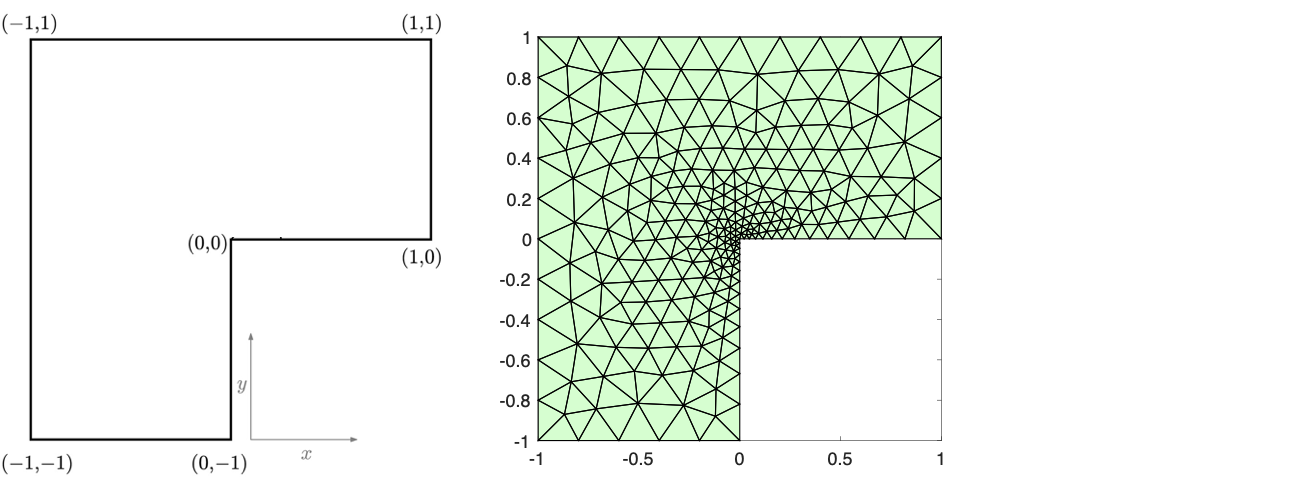
\includegraphics[scale=1.54]{lshape.png} \\
\label{fig2}
\end{center}
Figure 2:   The L-shaped domain and its finite element mesh generated by Gmsh from the geometry model file \textcolor{orange}{lshape.geo}. 
\end{figure}

\subsection{Finite Element Mesh}

A finite element mesh of a geometry model is a tessellation of its geometry by simple geometrical elements of various shapes such as lines, triangles, quadrangles, tetrahedra, prisms, hexahedra and pyramids. \texttt{Exasim} can handle conformal finite element meshes of triangular, quadrilateral, tetrahedra, and hexahedra elements.  In \texttt{Exasim}, a finite element mesh is composed of $p$ and $t$, where $p \in \mathbb{R}^{n_d \times n_p}$ is a two-dimensional float array storing mesh points and $t \in \mathbb{I}^{n_{ve} \times n_e}$  is a two-dimensional integer array storing mesh elements. Here $n_p$ is the number of mesh points, $n_{ve}$ is the number of vertices of an element, and $n_e$ is the number of elements. There are three different ways to input a finite element mesh into \texttt{Exasim}. First, \texttt{Exasim} has a Mesh module to generate meshes for some simple geometries.

Second, \texttt{Exasim}  uses Gmsh to  generate meshes from a geometry model file and mesh size parameters specified in the geometry model file, says \textcolor{orange}{filename.geo}, through the following function
\begin{tcolorbox}[breakable, size=fbox, boxrule=1pt, pad at break*=1mm,colback=cellbackground, colframe=cellborder]
\begin{Verbatim}[commandchars=\\\{\}]
\PY{c}{\PYZsh{} Call Gmsh to generate a mesh for a domain described in the file filename.geo}
\PY{n}{p}\PY{p}{,} \PY{n}{t} \PY{o}{=} \PY{n}{Mesh}\PY{o}{.}\PY{n}{gmshcall}\PY{p}{(}\PY{n}{pde}\PY{p}{,} \PY{l+s}{\PYZdq{}}\PY{l+s}{f}\PY{l+s}{i}\PY{l+s}{l}\PY{l+s}{e}\PY{l+s}{n}\PY{l+s}{a}\PY{l+s}{m}\PY{l+s}{e}\PY{l+s}{\PYZdq{}}\PY{p}{,} \PY{n}{nd}\PY{p}{,} \PY{n}{elemtype}\PY{p}{)}\PY{p}{;}
\end{Verbatim}
\end{tcolorbox}
where nd is the dimensionality of the physical domain and elemtype denotes the type of elements. In \texttt{Exasim}, elemtype = 0 means triangles in 2D and tetrahedra in 3D,  and elemtype = 1 means quadrilaterals in 2D and hexahedra in 3D. Note that file extension ".geo" must be excluded. Figure 2 shows a finite element mesh generated by Gmsh for the L-shaped domain defined in  \textcolor{orange}{lshape.geo}. 

And third, a finite element mesh can be imported into \texttt{Exasim} via either a text file or binary file as follows
\begin{tcolorbox}[breakable, size=fbox, boxrule=1pt, pad at break*=1mm,colback=cellbackground, colframe=cellborder]
\begin{Verbatim}[commandchars=\\\{\}]
\PY{c}{\PYZsh{} Read a mesh from an input file}
\PY{n}{p}\PY{p}{,} \PY{n}{t} \PY{o}{=} \PY{n}{Mesh}\PY{o}{.}\PY{n}{readmesh}\PY{p}{(}\PY{l+s}{\PYZdq{}}\PY{l+s}{f}\PY{l+s}{i}\PY{l+s}{l}\PY{l+s}{e}\PY{l+s}{n}\PY{l+s}{a}\PY{l+s}{m}\PY{l+s}{e}\PY{l+s}{.}\PY{l+s}{e}\PY{l+s}{x}\PY{l+s}{t}\PY{l+s}{\PYZdq{}}\PY{p}{,} \PY{n}{mode}\PY{p}{)}\PY{p}{;}
\end{Verbatim}
\end{tcolorbox}
Here mode can be either 0 (binary) or 1 (ascii). Both a filename and its extension must be provided. Below is the format of Exasim's text mesh file 

    \begin{tcolorbox}[breakable, size=fbox, boxrule=1pt, pad at break*=1mm,colback=cellbackground, colframe=cellborder]
\begin{Verbatim}[commandchars=\\\{\}]
\PY{n}{nd} \PY{n}{np} \PY{n}{nve} \PY{n}{ne}
\PY{n}{p}\PY{p}{[}\PY{l+m+mi}{1}\PY{p}{,}\PY{l+m+mi}{1}\PY{p}{]} \PY{n}{p}\PY{p}{[}\PY{l+m+mi}{1}\PY{p}{,}\PY{l+m+mi}{2}\PY{p}{]} \PY{o}{.}\PY{o}{.}\PY{o}{.} \PY{n}{p}\PY{p}{[}\PY{l+m+mi}{1}\PY{p}{,}\PY{n}{nd}\PY{p}{]}
\PY{n}{p}\PY{p}{[}\PY{l+m+mi}{2}\PY{p}{,}\PY{l+m+mi}{1}\PY{p}{]} \PY{n}{p}\PY{p}{[}\PY{l+m+mi}{2}\PY{p}{,}\PY{l+m+mi}{2}\PY{p}{]} \PY{o}{.}\PY{o}{.}\PY{o}{.} \PY{n}{p}\PY{p}{[}\PY{l+m+mi}{2}\PY{p}{,}\PY{n}{nd}\PY{p}{]}
\PY{o}{.}\PY{o}{.}\PY{o}{.}
\PY{n}{p}\PY{p}{[}\PY{n}{np}\PY{p}{,}\PY{l+m+mi}{1}\PY{p}{]} \PY{n}{p}\PY{p}{[}\PY{n}{np}\PY{p}{,}\PY{l+m+mi}{2}\PY{p}{]} \PY{o}{.}\PY{o}{.}\PY{o}{.} \PY{n}{p}\PY{p}{[}\PY{n}{np}\PY{p}{,}\PY{n}{nd}\PY{p}{]}
\PY{n}{t}\PY{p}{[}\PY{l+m+mi}{1}\PY{p}{,}\PY{l+m+mi}{1}\PY{p}{]} \PY{n}{t}\PY{p}{[}\PY{l+m+mi}{1}\PY{p}{,}\PY{l+m+mi}{2}\PY{p}{]} \PY{o}{.}\PY{o}{.}\PY{o}{.} \PY{n}{t}\PY{p}{[}\PY{l+m+mi}{1}\PY{p}{,}\PY{n}{nve}\PY{p}{]}
\PY{n}{t}\PY{p}{[}\PY{l+m+mi}{2}\PY{p}{,}\PY{l+m+mi}{1}\PY{p}{]} \PY{n}{t}\PY{p}{[}\PY{l+m+mi}{2}\PY{p}{,}\PY{l+m+mi}{2}\PY{p}{]} \PY{o}{.}\PY{o}{.}\PY{o}{.} \PY{n}{t}\PY{p}{[}\PY{l+m+mi}{2}\PY{p}{,}\PY{n}{nve}\PY{p}{]}
\PY{o}{.}\PY{o}{.}\PY{o}{.}
\PY{n}{t}\PY{p}{[}\PY{n}{ne}\PY{p}{,}\PY{l+m+mi}{1}\PY{p}{]} \PY{n}{t}\PY{p}{[}\PY{n}{ne}\PY{p}{,}\PY{l+m+mi}{2}\PY{p}{]} \PY{o}{.}\PY{o}{.}\PY{o}{.} \PY{n}{t}\PY{p}{[}\PY{n}{ne}\PY{p}{,}\PY{n}{nve}\PY{p}{]}
\end{Verbatim}
\end{tcolorbox}

The first line of the mesh file consists of four integers which are  $n_d$, $n_p$, $n_{ve}$, and $n_e$, respectively. The next $n_p$ lines store the coordinates for each of the mesh points.  The last $n_e$ lines store the element connectivities for each of the mesh elements. The format of the binary mesh file follows that of the text mesh file. It is important to note that all the entries in the binary mesh file are treated as double (float64) type. \texttt{Exasim} will read the $t$ array from the binary file as double array and convert $it$ into integer array. 


 \subsection{High-Order Finite Element Mesh}
 
The array tuple $(p, t)$  represents a standard finite element mesh. Since \texttt{Exasim} uses high-order DG methods for spatial discretization of PDEs, it creates a high-order mesh from a standard finite element mesh $(p,t)$. In \texttt{Exasim}, a high-order mesh has the following data structure: 
 
\begin{tcolorbox}[breakable, size=fbox, boxrule=1pt, pad at break*=1mm,colback=cellbackground, colframe=cellborder]
\begin{Verbatim}[commandchars=\\\{\}]
\PY{k}{mutable} \PY{k}{struct} \PY{n}{MeshStruct}
    \PY{n}{p}\PY{o}{::}\PY{k+kt}{Array}\PY{p}{\PYZob{}}\PY{n}{Float64}\PY{p}{,}\PY{l+m+mi}{2}\PY{p}{\PYZcb{}}\PY{p}{;}       \PY{c}{\PYZsh{} points of a linear mesh}
    \PY{n}{t}\PY{o}{::}\PY{k+kt}{Array}\PY{p}{\PYZob{}}\PY{n}{Int64}\PY{p}{,}\PY{l+m+mi}{2}\PY{p}{\PYZcb{}}\PY{p}{;}         \PY{c}{\PYZsh{} elements of a linear mesh}
    \PY{n}{boundaryexpr}\PY{p}{;}             \PY{c}{\PYZsh{} expressions to determine boundaries}
    \PY{n}{boundarycondition}\PY{o}{::}\PY{k+kt}{Array}\PY{p}{\PYZob{}}\PY{n}{Int64}\PY{p}{,}\PY{l+m+mi}{2}\PY{p}{\PYZcb{}}\PY{p}{;} \PY{c}{\PYZsh{} a list of boundary conditions}
    \PY{n}{curvedboundary}\PY{o}{::}\PY{k+kt}{Array}\PY{p}{\PYZob{}}\PY{n}{Int64}\PY{p}{,}\PY{l+m+mi}{2}\PY{p}{\PYZcb{}}\PY{p}{;} \PY{c}{\PYZsh{} boolean flags for curved boundaries}    
    \PY{n}{curvedboundaryexpr}\PY{p}{;}       \PY{c}{\PYZsh{} expressions to determine curved boundaries}
    \PY{n}{periodicexpr}\PY{p}{;}      	\PY{c}{\PYZsh{} expressions to map periodic boundaries}    
    \PY{n}{f}\PY{o}{::}\PY{k+kt}{Array}\PY{p}{\PYZob{}}\PY{n}{Int64}\PY{p}{,}\PY{l+m+mi}{2}\PY{p}{\PYZcb{}}\PY{p}{;}         \PY{c}{\PYZsh{} faces of a linear mesh}
    \PY{n}{tprd}\PY{o}{::}\PY{k+kt}{Array}\PY{p}{\PYZob{}}\PY{n}{Int64}\PY{p}{,}\PY{l+m+mi}{2}\PY{p}{\PYZcb{}}\PY{p}{;}      \PY{c}{\PYZsh{} elements for periodic conditions}    
    \PY{n}{dgnodes}\PY{o}{::}\PY{k+kt}{Array}\PY{p}{\PYZob{}}\PY{n}{Float64}\PY{p}{,}\PY{l+m+mi}{3}\PY{p}{\PYZcb{}}\PY{p}{;} \PY{c}{\PYZsh{} spatial nodes of a high\PYZhy{}order mesh}    
\PY{k}{end}
\end{Verbatim}
\end{tcolorbox}

Here \PY{n}{boundaryexpr} = [$b_1(\bm x)$, $b_2(\bm x)$, \ldots, $b_{n_{bc}}(\bm x)$] is a {\em priority} list of $n_{bc}$ user-specified boolean functions to divide the whole physical boundary $\partial \Omega$ into $n_{bc}$ disjoint boundaries $\Gamma_j, 1 \le j \le n_{bc}$, such that $\overline{\partial \Omega} = \cup_{j=1}^{n_{bc}} \overline{\Gamma}_{j}$. In particular,  if any point $\bm x \in \partial \Omega$ satisfies $b_1(\bm x)$ == True, then it belongs to $\Gamma_1$. Next, if $\bm x \in \partial \Omega$ satisfies $b_2(\bm x)$ == True, then it belongs to $\Gamma_2$. So on, until if $\bm x \in \partial \Omega$ satisfies $b_{n_{bc}}(\bm x)$ == True, then it belongs to $\Gamma_{n_{bc}}$. Note that if $\bm {x} \in \partial \Omega$ satisfies $b_2(\bm x)$ == True, $b_4(\bm x)$ == True, and $b_5(\bm x)$ == True, then it belongs to $\Gamma_{2}$. In other words, the first boolean function gets the first priority and the last boolean function gets the last priority. This allows us to apply boundary conditions to disjoint boundaries $\Gamma_j, 1 \le j \le n_{bc}$. Note that each disjoint boundary accepts only one boundary condition. 

Next, \PY{n}{boundarycondition} = [$c_1$, $c_2$, \ldots, $c_{n_{bc}}$] is an integer array of $n_{bc}$ entries which determine a boundary condition for each disjoint boundary. Specifically, disjoint boundary $\Gamma_j$ accepts boundary condition $c_j$. Assume that we divide the domain boundary $\partial \Omega$ into 4 disjoint boundaries $\Gamma_1,\ldots,\Gamma_4$ and that  \PY{n}{boundarycondition} = [2, 3, 1, 2]. In this case, $\Gamma_1$ accepts boundary condition 2,  $\Gamma_2$ accepts boundary condition 3,   $\Gamma_3$ accepts boundary condition 1, and  $\Gamma_4$ accepts boundary condition 2. Note that boundary condition 1, boundary condition 2, and boundary condition 3 must be implemented in {\em ubou} and {\em fbou} functions as discussed in the previous section. In other words,  \PY{n}{boundarycondition} is tied to the implementation of boundary conditions in {\em ubou} and {\em fbou} functions.

Next, \PY{n}{curvedboundary} = [$d_1$, $d_2$, \ldots, $d_{n_{bc}}$] is a boolean array of $n_{bc}$ entries which determine whether a disjoint boundary is curved or straight. Specifically, disjoint boundary $\Gamma_j$ is curved if $d_j = 1$ or straight if $d_j = 0$.  And \PY{n}{curvedboundaryexpr}  = [$s_1(\bm x)$, $s_2(\bm x)$, \ldots, $s_{n_{bc}}(\bm x)$]  is a list of  $n_{bc}$ functions that express the curved equation $s_j(\bm x) = 0$ for the disjoint boundary $\Gamma_j$. If $\Gamma_j$ is straight then both $d_j$  and $s_j(\bm x)$ are set to 0. Otherwise, if $\Gamma_j$ is curved then $d_j$ is set to 1 and the function $s_j(\bm x)$ must be specified. For example, if $\Gamma_j$ is a unit circle, then $s_j(\bm x) = x_1^2 + x_2^2 - 1$. \texttt{Exasim} uses \PY{n}{curvedboundary} and  \PY{n}{curvedboundaryexpr} to create high-order elements for the curved boundaries. Figure 3 shows an example of a standard finite element mesh and a high-order mesh generated by \texttt{Exasim}.

\begin{figure}[htbp]
\begin{center}
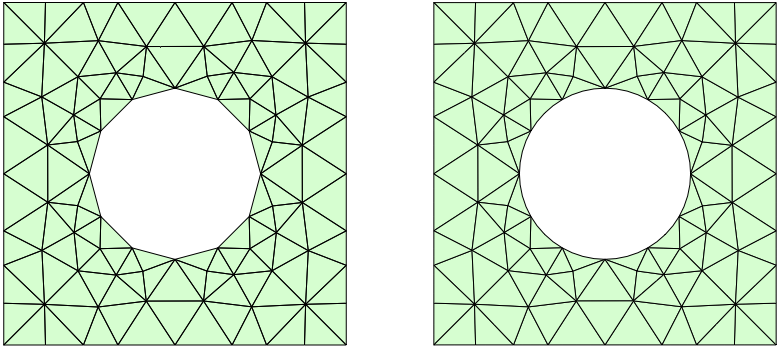
\includegraphics[scale=1.1]{curvedmesh.png} \\
\label{fig2}
\end{center}
Figure 3: Standard finite element mesh (left) and high-order mesh (right) for a domain bounded by a unit circle and a square. 
\end{figure}


Next, \PY{n}{periodicexpr} = [[$e_{11}$,  $p_{11}(\bm x)$, $e_{12}$, $p_{12}(\bm x)$],  \ldots, [$e_{n_{periodic} 1}$, $p_{n_{periodic} 1}(\bm x)$, $e_{n_{periodic} 2}$,$p_{n_{periodic} 2}(\bm x)$]] is a two-dimensional list of $n_{periodic} \times 4$ entries which determine a set of $n_{periodic}$ periodic boundary conditions. Each periodic boundary condition requires two disjoint boundaries. When two disjoint boundaries are periodic with each other,  there must be a one-to-one relationship for every mesh point on these two boundaries. This requirement must be met by a standard finite element mesh $(p,t)$. Hence, periodic boundary conditions place constraints on generating mesh points on periodic boundaries. For example, if \PY{n}{periodicexpr} = [[1, $p_{11}(\bm x)$, 3, $p_{12}(\bm x)$], [2, $p_{21}(\bm x)$, 4, $p_{22}(\bm x)$]], then $\Gamma_1$ (respectively, $\Gamma_2$) is periodic to $\Gamma_3$ (respectively, $\Gamma_4$) and any mesh point on $\Gamma_1$ (respectively, $\Gamma_2$) can be mapped to a mesh point on $\Gamma_3$ (respectively, $\Gamma_4$) by a mapping function, vice versa. The mapping functions $p_{11}(\bm x)$ and $p_{12}(\bm x)$, (respectively, $p_{21}(\bm x)$ and $p_{21}(\bm x)$) determine how two disjoint boundaries $\Gamma_1$  and $\Gamma_3$ (respectively, $\Gamma_2$ and $\Gamma_4$) are periodic each other. For example, in two dimensions, if $p_{11}(\bm x) = x_2$ and $p_{12}(\bm x) = x_2$ then every mesh point on $\Gamma_{1}$ must have its second coordinate equal to the second coordinate of one and only one mesh point on $\Gamma_{3}$. In three dimensions,  if $p_{11}(\bm x) = [x_2,x_3]$ and $p_{12}(\bm x) = \bm [x_2,x_3]$ then $\Gamma_{1}$ and $\Gamma_{3}$ are periodic with respect to $(x_2,x_3)$ coordinates.


% And \PY{n}{periodicexpr}  = [[$p_{11}(\bm x)$, $p_{12}(\bm x)$], \ldots, [$p_{n_{periodic} 1}(\bm x)$, $p_{n_{periodic} 2}(\bm x)$]]  is a list of  $n_{periodic} \times 2$ mapping functions that determine how two disjoint boundaries are periodic each other. For example, in two dimensions, if $p_{11}(\bm x) = x_2$ and $p_{12}(\bm x) = x_2$ then every mesh point on $\Gamma_{e_{11}}$ must have its second coordinate equal to the second coordinate of one and only one mesh point on $\Gamma_{e_{12}}$. In three dimensions,  if $p_{11}(\bm x) = [x_2,x_3]$ and $p_{12}(\bm x) = \bm [x_2,x_3]$ then $\Gamma_{e_{11}}$ and $\Gamma_{e_{12}}$ are periodic with respect to $(x_2,x_3)$ coordinates.

%Next, \PY{n}{periodicboundary} = [[$e_{11}$, $e_{12}$], [$e_{21}$, $e_{22}$], \ldots, [$e_{n_{periodic} 1}$, $e_{n_{periodic} 2}$]] is a two-dimensional integer array of $n_{periodic} \times 2$ entries which determine a set of $n_{periodic}$ periodic boundary conditions. Each periodic boundary condition requires two disjoint boundaries. When two disjoint boundaries are periodic with each other,  there must be a one-to-one relationship for every mesh point on these two boundaries. This requirement must be met by a standard finite element mesh $(p,t)$. Hence, periodic boundary conditions place constraints on generating mesh points on periodic boundaries. For example, if \PY{n}{periodicboundary} = [[1, 3], [2, 4]], then $\Gamma_1$ (respectively, $\Gamma_2$) is periodic to $\Gamma_3$ (respectively, $\Gamma_4$) and any mesh point on $\Gamma_1$ (respectively, $\Gamma_2$) can be mapped to a mesh point on $\Gamma_3$ (respectively, $\Gamma_4$) by a mapping function, vice versa.  And \PY{n}{periodicexpr}  = [[$p_{11}(\bm x)$, $p_{12}(\bm x)$], \ldots, [$p_{n_{periodic} 1}(\bm x)$, $p_{n_{periodic} 2}(\bm x)$]]  is a list of  $n_{periodic} \times 2$ mapping functions that determine how two disjoint boundaries are periodic each other. For example, in two dimensions, if $p_{11}(\bm x) = x_2$ and $p_{12}(\bm x) = x_2$ then every mesh point on $\Gamma_{e_{11}}$ must have its second coordinate equal to the second coordinate of one and only one mesh point on $\Gamma_{e_{12}}$. In three dimensions,  if $p_{11}(\bm x) = [x_2,x_3]$ and $p_{12}(\bm x) = \bm [x_2,x_3]$ then $\Gamma_{e_{11}}$ and $\Gamma_{e_{12}}$ are periodic with respect to $(x_2,x_3)$ coordinates.

Next, \PY{n}{f} is an integer array of size $n_{fe} \times n_{e}$, where $n_{fe}$ is the number of faces of an element. It indicates if a face is inside the physical domain or on disjoint boundaries. Note that \PY{n}{f} is determined by \texttt{Exasim} from \PY{n}{mesh}\PY{o}{.}\PY{n}{boundaryexpr}.

Next, \PY{n}{tprd} is an integer array of size $n_{ve} \times n_{e}$. So, \PY{n}{tprd} is the same size as $t$ and contains element connectivities for handling periodic boundary conditions. When there are periodic boundaries, the element connectivities need to be updated by \texttt{Exasim}.
 
Finally, \PY{n}{dgnodes} is a float array of size $n_{pe} \times n_{d} \times n_{e}$ storing mesh points to represent high-order elements, where $n_{pe}$ is the number of polynomials per element. Note that \PY{n}{dgnodes}  depends on  the polynomial degree and the element shape, and that it is computed by \texttt{Exasim}. The ordering of mesh points for the  high-order master element is based on the following rule: mesh points along the first coordinate $x_1$ are listed before those along the second $x_2$ and third $x_3$ coordinates; and mesh points along the second coordinate $x_2$ are listed before those along the third $x_3$ coordinate. %Figure 3 shows mesh points of a high-order mesh.


% Specification of \PY{n}{mesh}\PY{o}{.}\PY{n}{bndexpr} depends on the geometry and the boundary conditions. For instance, in the below example, \PY{n}{mesh}\PY{o}{.}\PY{n}{bndexpr} produces four boundaries (in the order of bottom, right, top, and left) for the unit square. \PY{n}{mesh}\PY{o}{.}\PY{n}{dgnodes} is a float array of size $n_{pe} \times n_{d} \times n_{e}$ storing nodal points to represent high-order elements, where $n_{pe}$ is the number of polynomials per element. Note that \PY{n}{mesh}\PY{o}{.}\PY{n}{dgnodes}  depends on  \PY{n}{app}\PY{o}{.}\PY{n}{porder} and the element type. It is computed by calling \PY{n}{mesh} \PY{o}{=} \PY{n}{Preprocessing}\PY{o}{.}\PY{n}{createhighordermesh}\PY{p}{(}\PY{n}{mesh}\PY{p}{,}\PY{n}{app}\PY{p}{)}\PY{p}.  \PY{n}{mesh}\PY{o}{.}\PY{n}{curvedboundary} is a boolean array of length $n_b$ indicating whether curved (= 1) or straight ( = 0) boundaries, where $n_b$ is the number of boundaries. In the below example, since the square has no curved boundary, all entries of \PY{n}{mesh}\PY{o}{.}\PY{n}{curvedboundary} are set to zero. 

%\begin{tcolorbox}[breakable, size=fbox, boxrule=1pt, pad at break*=1mm,colback=cellbackground, colframe=cellborder]
%\begin{Verbatim}[commandchars=\\\{\}]
%\PY{c}{\PYZsh{} create a linear mesh}
%\PY{n}{m} \PY{o}{=} \PY{l+m+mi}{8}\PY{p}{;} \PY{n}{n} \PY{o}{=} \PY{l+m+mi}{8}\PY{p}{;} \PY{c}{\PYZsh{} m by n grid of the square}
%\PY{n}{elemtype} \PY{o}{=} \PY{l+m+mi}{1}\PY{p}{;} \PY{c}{\PYZsh{} quad elements}
%\PY{n}{mesh} \PY{o}{=} \PY{n}{Structs}\PY{o}{.}\PY{n}{MeshStruct}\PY{p}{(}\PY{p}{)}\PY{p}{;}
%\PY{n}{mesh}\PY{o}{.}\PY{n}{p}\PY{p}{,}\PY{n}{mesh}\PY{o}{.}\PY{n}{t} \PY{o}{=} \PY{n}{Mesh}\PY{o}{.}\PY{n}{SquareMesh}\PY{p}{(}\PY{n}{m}\PY{p}{,}\PY{n}{n}\PY{p}{,}\PY{n}{elemtype}\PY{p}{)}\PY{p}{;}
%\PY{c}{\PYZsh{} expressions for domain boundaries}
%\PY{n}{mesh}\PY{o}{.}\PY{n}{bndexpr} \PY{o}{=} \PY{p}{[}\PY{n}{p} \PY{o}{\PYZhy{}}\PY{o}{\PYZgt{}} \PY{p}{(}\PY{n}{p}\PY{p}{[}\PY{l+m+mi}{2}\PY{p}{,}\PY{o}{:}\PY{p}{]} \PY{o}{.\PYZlt{}} \PY{l+m+mf}{1e\PYZhy{}3}\PY{p}{)}\PY{p}{,} \PY{n}{p} \PY{o}{\PYZhy{}}\PY{o}{\PYZgt{}} \PY{p}{(}\PY{n}{p}\PY{p}{[}\PY{l+m+mi}{1}\PY{p}{,}\PY{o}{:}\PY{p}{]} \PY{o}{.\PYZgt{}} \PY{l+m+mi}{1}\PY{o}{\PYZhy{}}\PY{l+m+mf}{1e\PYZhy{}3}\PY{p}{)}\PY{p}{,} \PY{n}{p} \PY{o}{\PYZhy{}}\PY{o}{\PYZgt{}} \PY{p}{(}\PY{n}{p}\PY{p}{[}\PY{l+m+mi}{2}\PY{p}{,}\PY{o}{:}\PY{p}{]} \PY{o}{.\PYZgt{}} \PY{l+m+mi}{1}\PY{o}{\PYZhy{}}\PY{l+m+mf}{1e\PYZhy{}3}\PY{p}{)}\PY{p}{,} \PY{n}{p} \PY{o}{\PYZhy{}}\PY{o}{\PYZgt{}} \PY{p}{(}\PY{n}{p}\PY{p}{[}\PY{l+m+mi}{1}\PY{p}{,}\PY{o}{:}\PY{p}{]} \PY{o}{.\PYZlt{}} \PY{l+m+mf}{1e\PYZhy{}3}\PY{p}{)}\PY{p}{]}\PY{p}{;}
%\PY{c}{\PYZsh{} expressions for curved boundaries}
%\PY{n}{mesh}\PY{o}{.}\PY{n}{curvedboundary} \PY{o}{=} \PY{p}{[}\PY{l+m+mi}{0} \PY{l+m+mi}{0} \PY{l+m+mi}{0} \PY{l+m+mi}{0}\PY{p}{]}\PY{p}{;}
%\PY{n}{mesh}\PY{o}{.}\PY{n}{curvedboundaryexpr} \PY{o}{=} \PY{p}{[}\PY{p}{]}\PY{p}{;}
%\PY{c}{\PYZsh{} experssions for periodic boundaries}
%\PY{n}{mesh}\PY{o}{.}\PY{n}{periodicexpr} \PY{o}{=} \PY{p}{[}\PY{p}{]}\PY{p}{;}
%\PY{c}{\PYZsh{} generate curved high\PYZhy{}order mesh from the linear mesh}
%\PY{n}{mesh} \PY{o}{=} \PY{n}{Preprocessing}\PY{o}{.}\PY{n}{createhighordermesh}\PY{p}{(}\PY{n}{mesh}\PY{p}{,}\PY{n}{app}\PY{p}{)}\PY{p}{;}
%\end{Verbatim}
%\end{tcolorbox}
%    
%If the domain has curved boundaries, the corresponding entries of \PY{n}{mesh}\PY{o}{.}\PY{n}{curvedboundary}  should be set to 1. Furthermore, the mathematical expressions for the curved boundaries should be provided in \PY{n}{mesh}\PY{o}{.}\PY{n}{curvedboundaryexpr}, so that they can be used to create high-order curved elements. Below is an example of creating a high-order mesh for a curved domain that has a hollow circle inside a solid square. 


\section{Exasim}

In this section, we describe how \texttt{Exasim} generate executable DG codes to solve parametrized PDE models. This is done by writing a script file in Julia, Python, or Matlab. Below is an example of a script file \textcolor{orange}{pdeapp.jl} for solving the 3D Poisson equation (\ref{poi3d}).

\subsection{3D Poisson Equation as ``Hello, World''}

\begin{tcolorbox}[breakable, size=fbox, boxrule=1pt, pad at break*=1mm,colback=cellbackground, colframe=cellborder]
\begin{Verbatim}[commandchars=\\\{\}]
\PY{c}{\PYZsh{} specify an Exasim version to run}
\PY{n}{version} \PY{o}{=} \PY{l+s}{\PYZdq{}}\PY{l+s}{V}\PY{l+s}{e}\PY{l+s}{r}\PY{l+s}{s}\PY{l+s}{i}\PY{l+s}{o}\PY{l+s}{n}\PY{l+s}{0}\PY{l+s}{.}\PY{l+s}{1}\PY{l+s}{\PYZdq{}}\PY{p}{;}

\PY{c}{\PYZsh{} External modules}
\PY{k}{using} \PY{n}{Revise}\PY{p}{,} \PY{n}{DelimitedFiles}\PY{p}{,} \PY{n}{SymPy}

\PY{c}{\PYZsh{} Add Exasim to Julia search path}
\PY{n}{cdir} \PY{o}{=} \PY{n}{pwd}\PY{p}{(}\PY{p}{)}\PY{p}{;} \PY{n}{ii} \PY{o}{=} \PY{n}{findlast}\PY{p}{(}\PY{l+s}{\PYZdq{}}\PY{l+s}{E}\PY{l+s}{x}\PY{l+s}{a}\PY{l+s}{s}\PY{l+s}{i}\PY{l+s}{m}\PY{l+s}{\PYZdq{}}\PY{p}{,} \PY{n}{cdir}\PY{p}{)}\PY{p}{;}
\PY{n}{include}\PY{p}{(}\PY{n}{cdir[1:ii[end]]} \PY{o}{*} \PY{l+s}{\PYZdq{}}\PY{l+s}{/Installation}\PY{l+s}{/}\PY{l+s}{s}\PY{l+s}{e}\PY{l+s}{t}\PY{l+s}{p}\PY{l+s}{a}\PY{l+s}{t}\PY{l+s}{h}\PY{l+s}{.}\PY{l+s}{j}\PY{l+s}{l}\PY{l+s}{\PYZdq{}}\PY{p}{)}\PY{p}{;}

\PY{c}{\PYZsh{} Exasim modules}
\PY{k}{using} \PY{n}{Preprocessing}\PY{p}{,} \PY{n}{Mesh}\PY{p}{,} \PY{n}{Gencode}\PY{p}{,} \PY{n}{Postprocessing}

\PY{c}{\PYZsh{} create pde structure and mesh structure}
\PY{n}{pde}\PY{p}{,} \PY{n}{mesh} \PY{o}{=} \PY{n}{Preprocessing}\PY{o}{.}\PY{n}{initializeexasim}\PY{p}{(}\PY{n}{version}\PY{p}{)}\PY{p}{;}

\PY{c}{\PYZsh{} Define PDE model: governing equations, initial and boundary conditions}
\PY{n}{pde}\PY{o}{.}\PY{n}{model} \PY{o}{=} \PY{l+s}{\PYZdq{}}\PY{l+s}{M}\PY{l+s}{o}\PY{l+s}{d}\PY{l+s}{e}\PY{l+s}{l}\PY{l+s}{D}\PY{l+s}{\PYZdq{}}\PY{p}{;}            \PY{c}{\PYZsh{} ModelC, ModelD, ModelW}
\PY{n}{include}\PY{p}{(}\PY{l+s}{\PYZdq{}}\PY{l+s}{p}\PY{l+s}{d}\PY{l+s}{e}\PY{l+s}{m}\PY{l+s}{o}\PY{l+s}{d}\PY{l+s}{e}\PY{l+s}{l}\PY{l+s}{.}\PY{l+s}{j}\PY{l+s}{l}\PY{l+s}{\PYZdq{}}\PY{p}{)}\PY{p}{;}          \PY{c}{\PYZsh{} include the PDE model file}

\PY{c}{\PYZsh{} Set discretization parameters, physical parameters, and solver parameters}
\PY{n}{pde}\PY{o}{.}\PY{n}{porder} \PY{o}{=} \PY{l+m+mi}{3}\PY{p}{;}                  \PY{c}{\PYZsh{} polynomial degree}
\PY{n}{pde}\PY{o}{.}\PY{n}{physicsparam} \PY{o}{=} \PY{p}{[}\PY{l+m+mf}{1.0} \PY{l+m+mf}{0.0}\PY{p}{]}\PY{p}{;}    \PY{c}{\PYZsh{} thermal conductivity and boundary value}
\PY{n}{pde}\PY{o}{.}\PY{n}{tau} \PY{o}{=} \PY{p}{[}\PY{l+m+mf}{1.0}\PY{p}{]}\PY{p}{;}                 \PY{c}{\PYZsh{} DG stabilization parameter}

\PY{c}{\PYZsh{} Choose computing platform and set number of processors}
\PY{c}{\PYZsh{}pde.platform = \PYZdq{}gpu\PYZdq{};           \PYZsh{} choose this option if running on Nvidia GPUs}
\PY{n}{pde}\PY{o}{.}\PY{n}{mpiprocs} \PY{o}{=} \PY{l+m+mi}{2}\PY{p}{;}                \PY{c}{\PYZsh{} number of MPI processors}

\PY{c}{\PYZsh{} create a linear mesh of 8 by 8 by 8 hexes on a unit cube}
\PY{n}{mesh}\PY{o}{.}\PY{n}{p}\PY{p}{,}\PY{n}{mesh}\PY{o}{.}\PY{n}{t} \PY{o}{=} \PY{n}{Mesh}\PY{o}{.}\PY{n}{cubemesh}\PY{p}{(}\PY{l+m+mi}{8}\PY{p}{,}\PY{l+m+mi}{8}\PY{p}{,}\PY{l+m+mi}{8}\PY{p}{,}\PY{l+m+mi}{1}\PY{p}{)}\PY{p}{;}
\PY{c}{\PYZsh{} expressions for disjoint boundaries}
\PY{n}{mesh}\PY{o}{.}\PY{n}{boundaryexpr} \PY{o}{=} \PY{p}{[}\PY{n}{p}\PY{o}{\PYZhy{}}\PY{o}{\PYZgt{}}\PY{p}{(}\PY{n}{p}\PY{p}{[}\PY{l+m+mi}{2}\PY{p}{,}\PY{o}{:}\PY{p}{]} \PY{o}{.\PYZlt{}} \PY{l+m+mf}{1e\PYZhy{}3}\PY{p}{)}\PY{p}{,} \PY{n}{p}\PY{o}{\PYZhy{}}\PY{o}{\PYZgt{}}\PY{p}{(}\PY{n}{p}\PY{p}{[}\PY{l+m+mi}{1}\PY{p}{,}\PY{o}{:}\PY{p}{]} \PY{o}{.\PYZgt{}} \PY{l+m+mi}{1}\PY{o}{\PYZhy{}}\PY{l+m+mf}{1e\PYZhy{}3}\PY{p}{)}\PY{p}{,} \PY{n}{p}\PY{o}{\PYZhy{}}\PY{o}{\PYZgt{}}\PY{p}{(}\PY{n}{p}\PY{p}{[}\PY{l+m+mi}{2}\PY{p}{,}\PY{o}{:}\PY{p}{]} \PY{o}{.\PYZgt{}} \PY{l+m+mi}{1}\PY{o}{\PYZhy{}}\PY{l+m+mf}{1e\PYZhy{}3}\PY{p}{)}\PY{p}{,} \PY{n}{p}\PY{o}{\PYZhy{}}\PY{o}{\PYZgt{}}\PY{p}{(}\PY{n}{p}\PY{p}{[}\PY{l+m+mi}{1}\PY{p}{,}\PY{o}{:}\PY{p}{]} \PY{o}{.\PYZlt{}} \PY{l+m+mf}{1e\PYZhy{}3}\PY{p}{)}\PY{p}{,} \PY{n}{p}\PY{o}{\PYZhy{}}\PY{o}{\PYZgt{}}\PY{p}{(}\PY{n}{p}\PY{p}{[}\PY{l+m+mi}{3}\PY{p}{,}\PY{o}{:}\PY{p}{]} \PY{o}{.\PYZlt{}} \PY{l+m+mf}{1e\PYZhy{}3}\PY{p}{)}\PY{p}{,} \PY{n}{p}\PY{o}{\PYZhy{}}\PY{o}{\PYZgt{}}\PY{p}{(}\PY{n}{p}\PY{p}{[}\PY{l+m+mi}{3}\PY{p}{,}\PY{o}{:}\PY{p}{]} \PY{o}{.\PYZgt{}} \PY{l+m+mi}{1}\PY{o}{\PYZhy{}}\PY{l+m+mf}{1e\PYZhy{}3}\PY{p}{)}\PY{p}{]}\PY{p}{;}
\PY{n}{mesh}\PY{o}{.}\PY{n}{boundarycondition} \PY{o}{=} \PY{p}{[}\PY{l+m+mi}{1} \PY{l+m+mi}{1} \PY{l+m+mi}{1} \PY{l+m+mi}{1} \PY{l+m+mi}{1} \PY{l+m+mi}{1}\PY{p}{]}\PY{p}{;} \PY{c}{\PYZsh{} Set boundary conditions}

\PY{c}{\PYZsh{} call Exasim to generate and run C++ code to solve the PDE model}
\PY{n}{sol}\PY{p}{,} \PY{n}{pde}\PY{p}{,} \PY{n}{mesh}\PY{p}{,} \PY{o}{\PYZti{}}\PY{p}{,}\PY{o}{\PYZti{}}\PY{p}{,}\PY{o}{\PYZti{}}\PY{p}{,}\PY{o}{\PYZti{}}  \PY{o}{=} \PY{n}{Postprocessing}\PY{o}{.}\PY{n}{exasim}\PY{p}{(}\PY{n}{pde}\PY{p}{,}\PY{n}{mesh}\PY{p}{)}\PY{p}{;}

\PY{c}{\PYZsh{} visualize the numerical solution of the PDE model using Paraview}
\PY{n}{pde}\PY{o}{.}\PY{n}{visscalars} \PY{o}{=} \PY{p}{[}\PY{l+s}{\PYZdq{}}\PY{l+s}{t}\PY{l+s}{e}\PY{l+s}{m}\PY{l+s}{p}\PY{l+s}{e}\PY{l+s}{r}\PY{l+s}{a}\PY{l+s}{t}\PY{l+s}{u}\PY{l+s}{r}\PY{l+s}{e}\PY{l+s}{\PYZdq{}}\PY{p}{,} \PY{l+m+mi}{1}\PY{p}{]}\PY{p}{;}  \PY{c}{\PYZsh{} list of scalar fields for visualization}
\PY{n}{pde}\PY{o}{.}\PY{n}{visvectors} \PY{o}{=} \PY{p}{[}\PY{l+s}{\PYZdq{}}\PY{l+s}{t}\PY{l+s}{e}\PY{l+s}{m}\PY{l+s}{p}\PY{l+s}{e}\PY{l+s}{r}\PY{l+s}{a}\PY{l+s}{t}\PY{l+s}{u}\PY{l+s}{r}\PY{l+s}{e}\PY{l+s}{ }\PY{l+s}{g}\PY{l+s}{r}\PY{l+s}{a}\PY{l+s}{d}\PY{l+s}{i}\PY{l+s}{e}\PY{l+s}{n}\PY{l+s}{t}\PY{l+s}{\PYZdq{}}\PY{p}{,} \PY{p}{[}\PY{l+m+mi}{2}\PY{p}{,} \PY{l+m+mi}{3}\PY{p}{,} \PY{l+m+mi}{4}\PY{p}{]}\PY{p}{]}\PY{p}{;} \PY{c}{\PYZsh{} list of vector fields}
\PY{n}{mesh}\PY{o}{.}\PY{n}{dgnodes} \PY{o}{=} \PY{n}{Postprocessing}\PY{o}{.}\PY{n}{vis}\PY{p}{(}\PY{n}{sol}\PY{p}{,}\PY{n}{pde}\PY{p}{,}\PY{n}{mesh}\PY{p}{)}\PY{p}{;} \PY{c}{\PYZsh{} visualize the solution}
\PY{n}{x} \PY{o}{=} \PY{n}{mesh}\PY{o}{.}\PY{n}{dgnodes}\PY{p}{[}\PY{o}{:}\PY{p}{,}\PY{l+m+mi}{1}\PY{p}{,}\PY{o}{:}\PY{p}{]}\PY{p}{;} \PY{n}{y} \PY{o}{=} \PY{n}{mesh}\PY{o}{.}\PY{n}{dgnodes}\PY{p}{[}\PY{o}{:}\PY{p}{,}\PY{l+m+mi}{2}\PY{p}{,}\PY{o}{:}\PY{p}{]}\PY{p}{;} \PY{n}{z} \PY{o}{=} \PY{n}{mesh}\PY{o}{.}\PY{n}{dgnodes}\PY{p}{[}\PY{o}{:}\PY{p}{,}\PY{l+m+mi}{3}\PY{p}{,}\PY{o}{:}\PY{p}{]}\PY{p}{;}
\PY{n}{uexact} \PY{o}{=} \PY{n}{sin}\PY{o}{.}\PY{p}{(}\PY{n+nb}{pi}\PY{o}{*}\PY{n}{x}\PY{p}{)}\PY{o}{.*}\PY{n}{sin}\PY{o}{.}\PY{p}{(}\PY{n+nb}{pi}\PY{o}{*}\PY{n}{y}\PY{p}{)}\PY{o}{.*}\PY{n}{sin}\PY{o}{.}\PY{p}{(}\PY{n+nb}{pi}\PY{o}{*}\PY{n}{z}\PY{p}{)}\PY{p}{;} \PY{c}{\PYZsh{} exact solution}
\PY{n}{uh} \PY{o}{=} \PY{n}{sol}\PY{p}{[}\PY{o}{:}\PY{p}{,}\PY{l+m+mi}{1}\PY{p}{,}\PY{o}{:}\PY{p}{]}\PY{p}{;}                             \PY{c}{\PYZsh{} numerical solution}
\PY{n}{maxerr} \PY{o}{=} \PY{n}{maximum}\PY{p}{(}\PY{n}{abs}\PY{o}{.}\PY{p}{(}\PY{n}{uh}\PY{p}{[}\PY{o}{:}\PY{p}{]}\PY{o}{\PYZhy{}}\PY{n}{uexact}\PY{p}{[}\PY{o}{:}\PY{p}{]}\PY{p}{)}\PY{p}{)}\PY{p}{;}
\PY{n}{print}\PY{p}{(}\PY{l+s}{\PYZdq{}}\PY{l+s}{M}\PY{l+s}{a}\PY{l+s}{x}\PY{l+s}{i}\PY{l+s}{m}\PY{l+s}{u}\PY{l+s}{m}\PY{l+s}{ }\PY{l+s}{a}\PY{l+s}{b}\PY{l+s}{s}\PY{l+s}{o}\PY{l+s}{l}\PY{l+s}{u}\PY{l+s}{t}\PY{l+s}{e}\PY{l+s}{ }\PY{l+s}{e}\PY{l+s}{r}\PY{l+s}{r}\PY{l+s}{o}\PY{l+s}{r}\PY{l+s}{:}\PY{l+s}{ }\PY{l+s+si}{\PYZdl{}maxerr}\PY{l+s+se}{\PYZbs{}n}\PY{l+s}{\PYZdq{}}\PY{p}{)}\PY{p}{;}
\PY{n}{print}\PY{p}{(}\PY{l+s}{\PYZdq{}}\PY{l+s}{D}\PY{l+s}{o}\PY{l+s}{n}\PY{l+s}{e}\PY{l+s}{!}\PY{l+s}{\PYZdq{}}\PY{p}{)}\PY{p}{;}
\end{Verbatim}
\end{tcolorbox}

This script file can be found in the folder \PY{I+s}{/Exasim/Applications/Poisson/Poisson3d}. In Julia REPL environment, when you go to this directory and run the script file as follows

\hspace{5ex} \PY{k}{julia>} include("pdeapp.jl")

The executable code \textbf{mpiapp} generated by \texttt{Exasim} can be found in the folder \PY{I+s}{app}. \texttt{Exasim} runs the code from Julia to solve the 3D Poisson equation (\ref{poi3d}). If all goes well, you should see the following lines in Julia REPL session. 

\begin{tcolorbox}[breakable, size=fbox, boxrule=1pt, pad at break*=1mm,colback=cellbackground, colframe=cellborder]
\begin{Verbatim}[commandchars=\\\{\}]
\PY{n}{generate} \PY{n}{code}\PY{o}{.}\PY{o}{.}\PY{o}{.}
\PY{n}{compile} \PY{n}{code}\PY{o}{.}\PY{o}{.}\PY{o}{.}
\PY{n}{run} \PY{n}{code}\PY{o}{.}\PY{o}{.}\PY{o}{.}
\PY{n}{Using} \PY{l+m+mi}{2} \PY{n}{processors} \PY{n}{to} \PY{n}{solve} \PY{n}{the} \PY{n}{problem} \PY{n}{on} \PY{n}{CPU} \PY{n}{platform}\PY{o}{.}\PY{o}{.}\PY{o}{.}
\PY{n}{Old} \PY{n}{RHS} \PY{n}{Norm}\PY{o}{:} \PY{l+m+mf}{0.0930155}\PY{p}{,}  \PY{n}{New} \PY{n}{RHS} \PY{n}{Norm}\PY{o}{:} \PY{l+m+mf}{0.0930155}
\PY{n}{GMRES} \PY{n}{converges} \PY{n}{to} \PY{n}{the} \PY{n}{tolerance} \PY{l+m+mf}{0.001} \PY{n}{within}  \PY{l+m+mi}{46} \PY{n}{iterations} \PY{n}{and} \PY{l+m+mi}{0} \PY{n}{RB} \PY{n}{dimensions}
\PY{n}{PTC} \PY{n}{Iteration}\PY{o}{:} \PY{l+m+mi}{1}\PY{p}{,}  \PY{n}{Residual} \PY{n}{Norm}\PY{o}{:} \PY{l+m+mf}{9.14294e\PYZhy{}05}
\PY{n}{Old} \PY{n}{RHS} \PY{n}{Norm}\PY{o}{:} \PY{l+m+mf}{9.14294e\PYZhy{}05}\PY{p}{,}  \PY{n}{New} \PY{n}{RHS} \PY{n}{Norm}\PY{o}{:} \PY{l+m+mf}{8.56196e\PYZhy{}05}
\PY{n}{GMRES} \PY{n}{converges} \PY{n}{to} \PY{n}{the} \PY{n}{tolerance} \PY{l+m+mf}{0.001} \PY{n}{within}  \PY{l+m+mi}{113} \PY{n}{iterations} \PY{n}{and} \PY{l+m+mi}{1} \PY{n}{RB} \PY{n}{dimensions}
\PY{n}{PTC} \PY{n}{Iteration}\PY{o}{:} \PY{l+m+mi}{2}\PY{p}{,}  \PY{n}{Residual} \PY{n}{Norm}\PY{o}{:} \PY{l+m+mf}{8.6313e\PYZhy{}08}
\PY{n}{Maximum} \PY{n}{absolute} \PY{n}{error}\PY{o}{:} \PY{l+m+mf}{4.792391576413646e\PYZhy{}5}
\PY{n}{Done!}
\end{Verbatim}
\end{tcolorbox}

In addition, \texttt{Exasim}  will open Paraview and visualize the numerical solution if Paraview is already installed on your computer. If Paraview is not installed, please install it and and add the following line 

\begin{tcolorbox}[breakable, size=fbox, boxrule=1pt, pad at break*=1mm,colback=cellbackground, colframe=cellborder]
\begin{Verbatim}[commandchars=\\\{\}]
\PY{c}{\PYZsh{} visualize the numerical solution of the PDE model using Paraview}
\PY{n}{pde}\PY{o}{.}\PY{n}{paraview} \PY{o}{=} \PY{l+s}{\PYZdq{}}\PY{l+s}{/}\PY{l+s}{p}\PY{l+s}{a}\PY{l+s}{t}\PY{l+s}{h}\PY{l+s}{/}\PY{l+s}{t}\PY{l+s}{o}\PY{l+s}{/}\PY{l+s}{p}\PY{l+s}{a}\PY{l+s}{r}\PY{l+s}{a}\PY{l+s}{v}\PY{l+s}{i}\PY{l+s}{e}\PY{l+s}{w}\PY{l+s}{/}\PY{l+s}{e}\PY{l+s}{x}\PY{l+s}{e}\PY{l+s}{c}\PY{l+s}{u}\PY{l+s}{t}\PY{l+s}{a}\PY{l+s}{b}\PY{l+s}{l}\PY{l+s}{e}\PY{l+s}{\PYZdq{}}\PY{p}{;}
\end{Verbatim}
\end{tcolorbox}

to the \textcolor{orange}{pdeapp}  script.  Here \PY{l+s}{\PYZdq{}}\PY{l+s}{/}\PY{l+s}{p}\PY{l+s}{a}\PY{l+s}{t}\PY{l+s}{h}\PY{l+s}{/}\PY{l+s}{t}\PY{l+s}{o}\PY{l+s}{/}\PY{l+s}{p}\PY{l+s}{a}\PY{l+s}{r}\PY{l+s}{a}\PY{l+s}{v}\PY{l+s}{i}\PY{l+s}{e}\PY{l+s}{w}\PY{l+s}{/}\PY{l+s}{e}\PY{l+s}{x}\PY{l+s}{e}\PY{l+s}{c}\PY{l+s}{u}\PY{l+s}{t}\PY{l+s}{a}\PY{l+s}{b}\PY{l+s}{l}\PY{l+s}{e}\PY{l+s}{\PYZdq{}} is the path to the Paraview executable file. For example, on MacOS systems, it can be \PY{l+s}{\PYZdq{}}\PY{l+s}{/}\PY{l+s}{A}\PY{l+s}{p}\PY{l+s}{p}\PY{l+s}{l}\PY{l+s}{i}\PY{l+s}{c}\PY{l+s}{a}\PY{l+s}{t}\PY{l+s}{i}\PY{l+s}{o}\PY{l+s}{n}\PY{l+s}{s}\PY{l+s}{/}\PY{l+s}{P}\PY{l+s}{a}\PY{l+s}{r}\PY{l+s}{a}\PY{l+s}{V}\PY{l+s}{i}\PY{l+s}{e}\PY{l+s}{w}\PY{l+s}{\PYZhy{}}\PY{l+s}{5}\PY{l+s}{.}\PY{l+s}{8}\PY{l+s}{.}\PY{l+s}{1}\PY{l+s}{.}\PY{l+s}{a}\PY{l+s}{p}\PY{l+s}{p}\PY{l+s}{/}\PY{l+s}{C}\PY{l+s}{o}\PY{l+s}{n}\PY{l+s}{t}\PY{l+s}{e}\PY{l+s}{n}\PY{l+s}{t}\PY{l+s}{s}\PY{l+s}{/}\PY{l+s}{M}\PY{l+s}{a}\PY{l+s}{c}\PY{l+s}{O}\PY{l+s}{S}\PY{l+s}{/}\PY{l+s}{p}\PY{l+s}{a}\PY{l+s}{r}\PY{l+s}{a}\PY{l+s}{v}\PY{l+s}{i}\PY{l+s}{e}\PY{l+s}{w}\PY{l+s}{\PYZdq{}} for Paraview version 5.8.1. Alternatively, you open the file \textcolor{orange}{initializepde.jl} in the folder \PY{I+s}{/Exasim/Version0.1/Julia/Preprocessing} and replace \PY{n}{pde}\PY{o}{.}\PY{n}{paraview} \PY{o}{=}   \PY{I+s}{"paraview"}  with the above line of code. If you use Matlab or Python, you can do likewise.

Once Paraview opens, click the Apply button and select  "temperature gradient", you should see Figure 4.

\begin{figure}[htbp]
\begin{center}
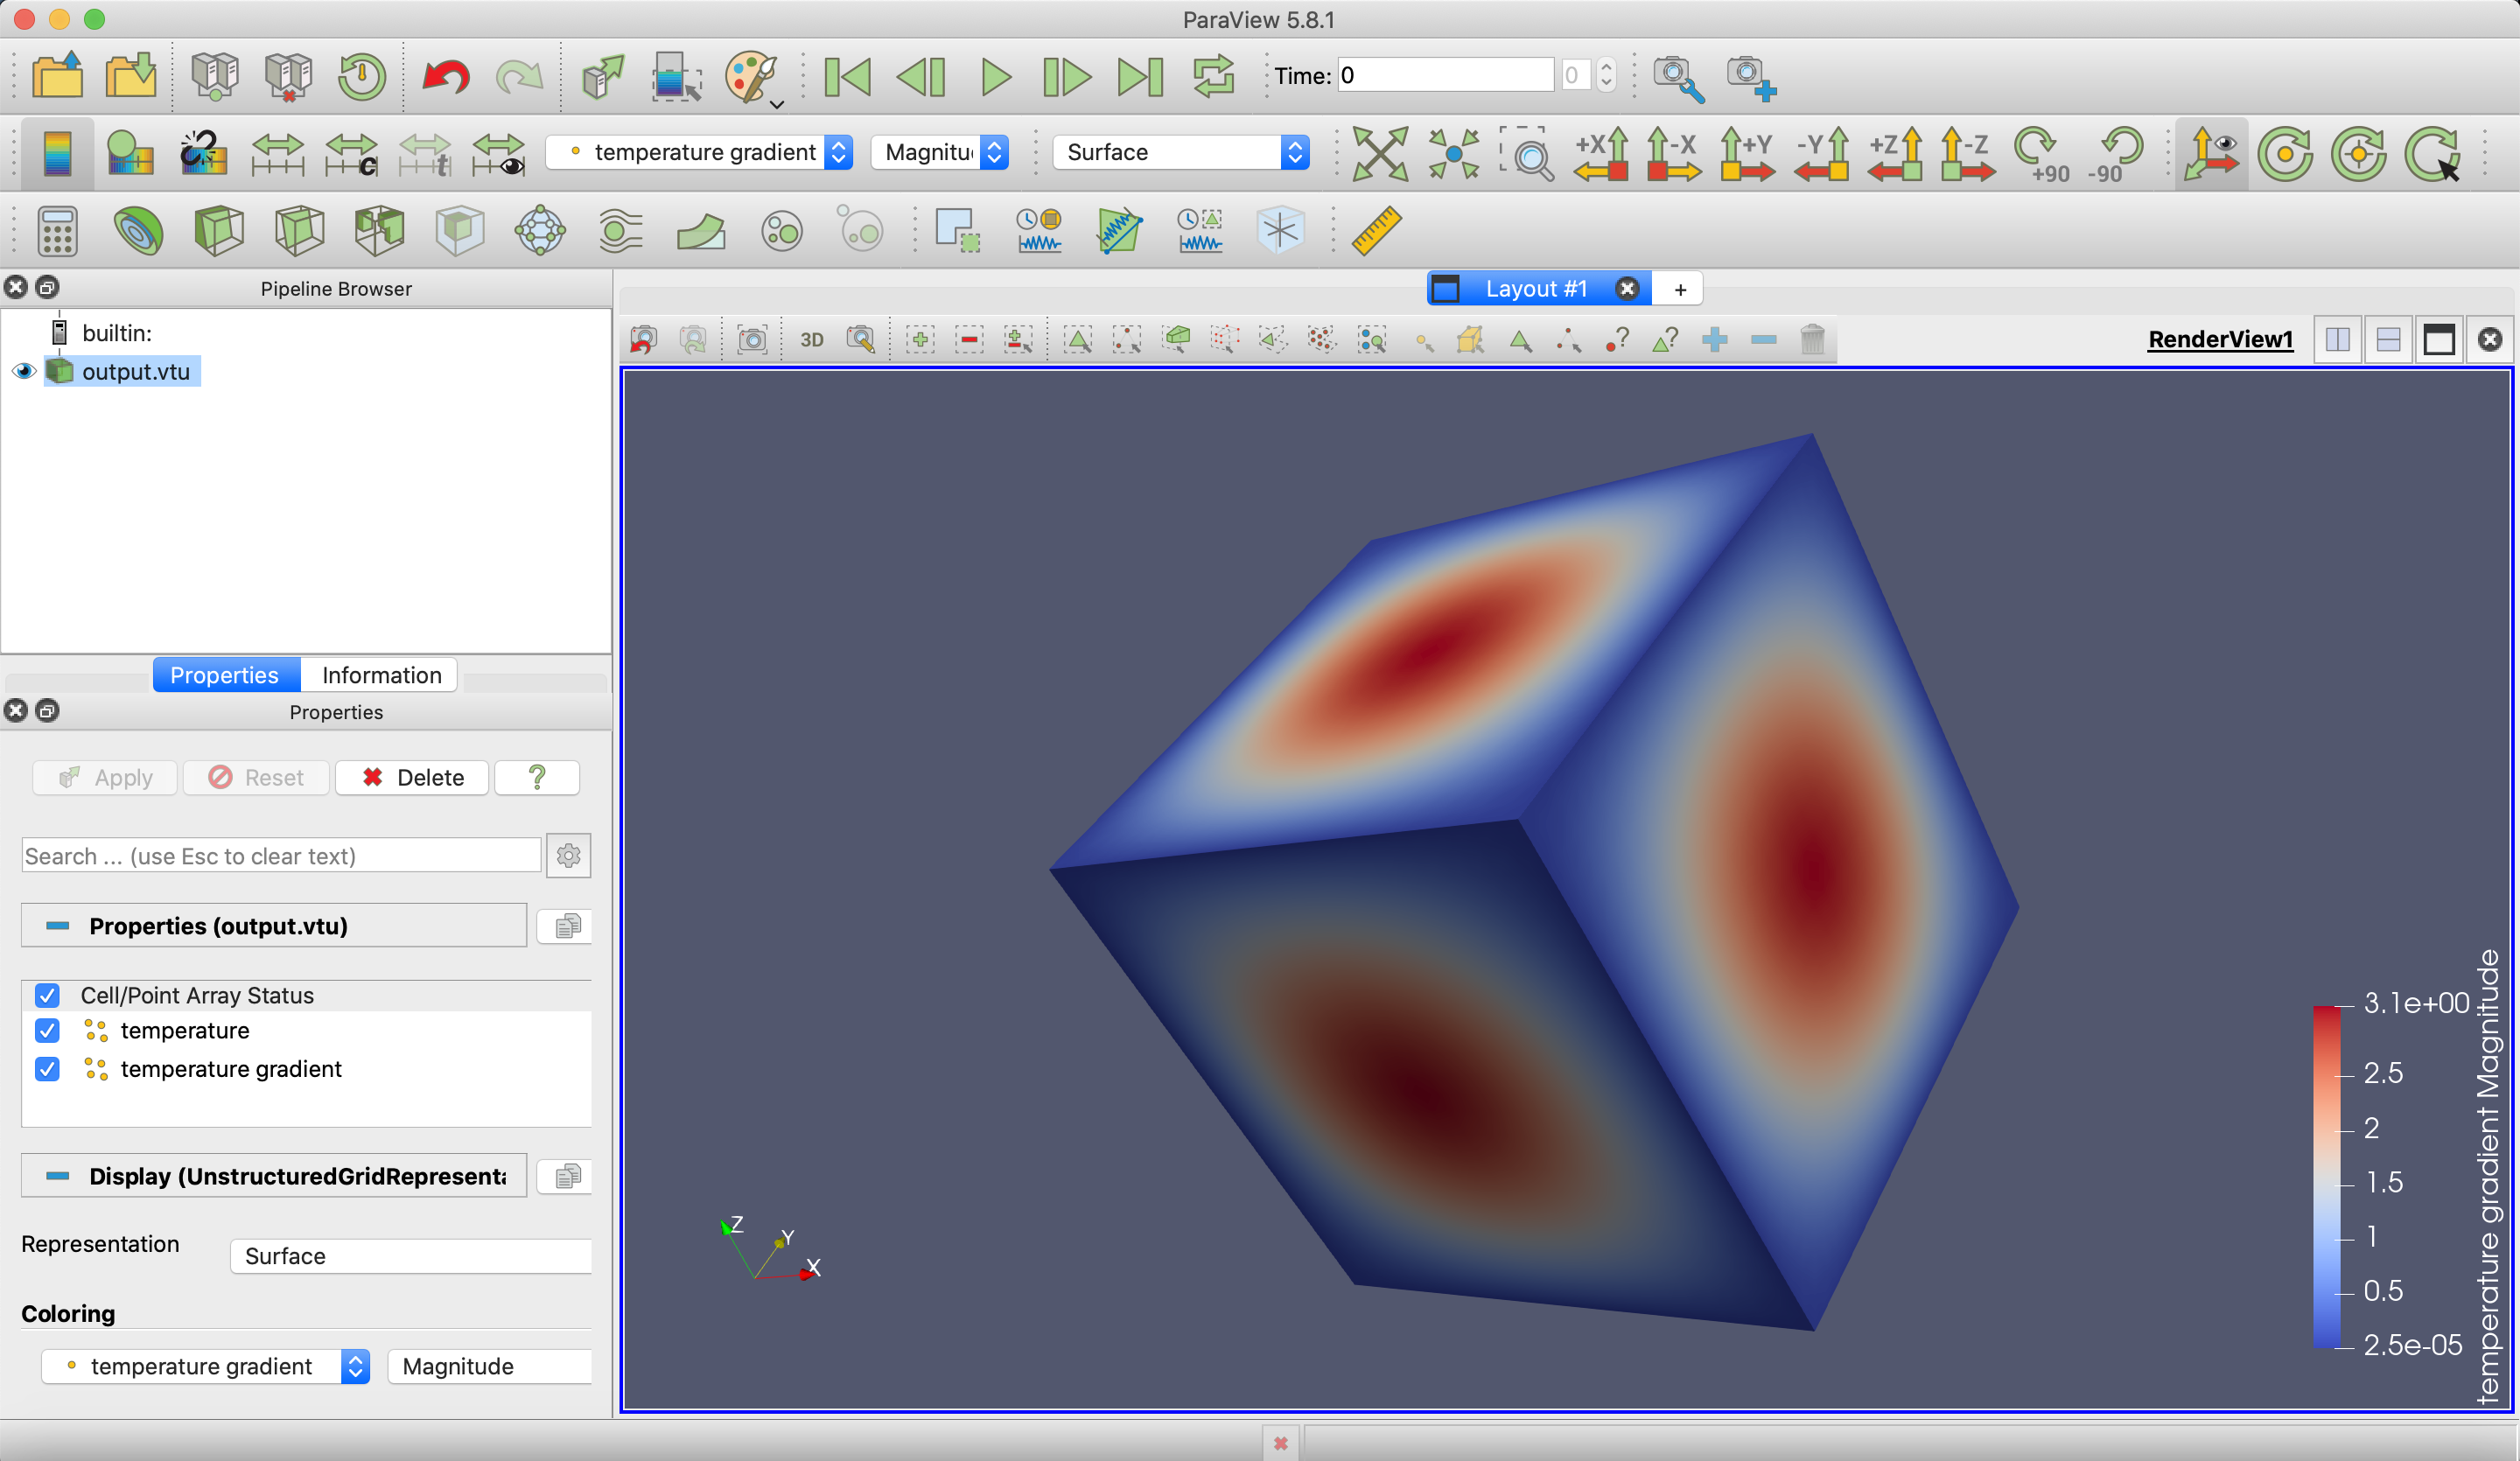
\includegraphics[scale=1.1]{paraview.png} \\
\label{fig4}
\end{center}
Figure 4: Visualize the numerical solution using Paraview. 
\end{figure}

As mentioned earlier, \texttt{Exasim} provides many examples that illustrate how to generate DG codes for solving a wide variety of PDEs including Poisson equation, wave equation, heat equation, advection, convection-diffusion, elasticity, Euler equations, Navier-Stokes equations, and MHD equations. These examples are placed in the folder \PY{I+s}{Exasim/Applications}. 


\subsection{Backward Compatibility}

\texttt{Exasim} is purposefully designed to make the code generator compatible with all of its future versions. The following line is placed at the top of any application script. 

\begin{tcolorbox}[breakable, size=fbox, boxrule=1pt, pad at break*=1mm,colback=cellbackground, colframe=cellborder]
\begin{Verbatim}[commandchars=\\\{\}]
\PY{c}{\PYZsh{} specify an Exasim version}
\PY{n}{version} \PY{o}{=} \PY{l+s}{\PYZdq{}}\PY{l+s}{V}\PY{l+s}{e}\PY{l+s}{r}\PY{l+s}{s}\PY{l+s}{i}\PY{l+s}{o}\PY{l+s}{n}\PY{l+s}{0}\PY{l+s}{.}\PY{l+s}{1}\PY{l+s}{\PYZdq{}}\PY{p}{;}
\end{Verbatim}
\end{tcolorbox}

If a new version of \texttt{Exasim} is released in the future,  only this line will be modified to the new version, while the rest of the script will stay the same.

\subsection{Exasim Modules}

Next,  the directories of \texttt{Exasim} modules are added to search path so that  they can be found.

\begin{tcolorbox}[breakable, size=fbox, boxrule=1pt, pad at break*=1mm,colback=cellbackground, colframe=cellborder]
\begin{Verbatim}[commandchars=\\\{\}]
\PY{c}{\PYZsh{} External modules}
\PY{k}{using} \PY{n}{Revise}\PY{p}{,} \PY{n}{DelimitedFiles}\PY{p}{,} \PY{n}{SymPy}

\PY{c}{\PYZsh{} Add Exasim to Julia search path}
\PY{n}{cdir} \PY{o}{=} \PY{n}{pwd}\PY{p}{(}\PY{p}{)}\PY{p}{;} \PY{n}{ii} \PY{o}{=} \PY{n}{findlast}\PY{p}{(}\PY{l+s}{\PYZdq{}}\PY{l+s}{E}\PY{l+s}{x}\PY{l+s}{a}\PY{l+s}{s}\PY{l+s}{i}\PY{l+s}{m}\PY{l+s}{\PYZdq{}}\PY{p}{,} \PY{n}{cdir}\PY{p}{)}\PY{p}{;}
\PY{n}{include}\PY{p}{(}\PY{n}{cdir[1:ii[end]]} \PY{o}{*} \PY{l+s}{\PYZdq{}}\PY{l+s}{/Installation}\PY{l+s}{/}\PY{l+s}{s}\PY{l+s}{e}\PY{l+s}{t}\PY{l+s}{p}\PY{l+s}{a}\PY{l+s}{t}\PY{l+s}{h}\PY{l+s}{.}\PY{l+s}{j}\PY{l+s}{l}\PY{l+s}{\PYZdq{}}\PY{p}{)}\PY{p}{;}

\PY{c}{\PYZsh{} Exasim modules}
\PY{k}{using} \PY{n}{Preprocessing}\PY{p}{,} \PY{n}{Mesh}\PY{p}{,} \PY{n}{Gencode}\PY{p}{,} \PY{n}{Postprocessing}
\end{Verbatim}
\end{tcolorbox}

\subsection{PDE Object and Mesh Object}

Next,  \texttt{Exasim} creates an object of PDE structure and an object of Mesh structure. The Mesh Structure is described in Section 3.3, while the PDE structure can be found in the file  \textcolor{orange}{intializepde}. Essentially, \texttt{Exasim} sets many default values to the pde object, while the mesh object is empty.

\begin{tcolorbox}[breakable, size=fbox, boxrule=1pt, pad at break*=1mm,colback=cellbackground, colframe=cellborder]
\begin{Verbatim}[commandchars=\\\{\}]
\PY{c}{\PYZsh{} create pde structure and mesh structure}
\PY{n}{pde}\PY{p}{,} \PY{n}{mesh} \PY{o}{=} \PY{n}{Preprocessing}\PY{o}{.}\PY{n}{initializeexasim}\PY{p}{(}\PY{n}{version}\PY{p}{)}\PY{p}{;}
\end{Verbatim}
\end{tcolorbox}



%\begin{tcolorbox}[breakable, size=fbox, boxrule=1pt, pad at break*=1mm,colback=cellbackground, colframe=cellborder]
%\begin{Verbatim}[commandchars=\\\{\}]
%\PY{k}{function} \PY{n}{initializeexasim}\PY{p}{(}\PY{n}{version}\PY{p}{)}
%
%\PY{c}{\PYZsh{} create a pde model object}
%\PY{n}{pde} \PY{o}{=} \PY{n}{Preprocessing}\PY{o}{.}\PY{n}{initializepde}\PY{p}{(}\PY{n}{version}\PY{p}{)}\PY{p}{;}
%
%\PY{c}{\PYZsh{} create a mesh object}
%\PY{n}{mesh} \PY{o}{=} \PY{n}{Preprocessing}\PY{o}{.}\PY{n}{initializemesh}\PY{p}{(}\PY{n}{version}\PY{p}{)}\PY{p}{;}
%
%\PY{k}{return} \PY{n}{pde}\PY{p}{,} \PY{n}{mesh}
%
%\PY{k}{end}
%\end{Verbatim}
%\end{tcolorbox}

\subsection{PDE Model File}

All application scripts have the previous lines of code and do not require any user's inputs up to this point. Next, we need to define a PDE model by writing a model file as described in Section 2.5. Once a PDE model file is written to express the governing equations, boundary conditions, and initial solutions of a specific PDE model, it must be included in the application script. Furthermore, it is required  to set \PY{n}{pde}\PY{o}{.}\PY{n}{model} to the correct PDE model type. As discussed in Section 2.5, \texttt{Exasim} supports three types of PDE models.  

\begin{tcolorbox}[breakable, size=fbox, boxrule=1pt, pad at break*=1mm,colback=cellbackground, colframe=cellborder]
\begin{Verbatim}[commandchars=\\\{\}]
\PY{c}{\PYZsh{} Define PDE model: governing equations, initial and boundary conditions}
\PY{n}{pde}\PY{o}{.}\PY{n}{model} \PY{o}{=} \PY{l+s}{\PYZdq{}}\PY{l+s}{M}\PY{l+s}{o}\PY{l+s}{d}\PY{l+s}{e}\PY{l+s}{l}\PY{l+s}{D}\PY{l+s}{\PYZdq{}}\PY{p}{;}            \PY{c}{\PYZsh{} ModelC, ModelD, ModelW}
\PY{n}{include}\PY{p}{(}\PY{l+s}{\PYZdq{}}\PY{l+s}{p}\PY{l+s}{d}\PY{l+s}{e}\PY{l+s}{m}\PY{l+s}{o}\PY{l+s}{d}\PY{l+s}{e}\PY{l+s}{l}\PY{l+s}{.}\PY{l+s}{j}\PY{l+s}{l}\PY{l+s}{\PYZdq{}}\PY{p}{)}\PY{p}{;}          \PY{c}{\PYZsh{} include the PDE model file}
\end{Verbatim}
\end{tcolorbox}


\subsection{Setting Parameters}

Next, we set physical parameters, discretization parameters, and solver parameters. The below parameters are always necessary. First, \PY{n}{pde}\PY{o}{.}\PY{n}{porder} is the degree of polynomials used to approximate the PDE solution on every element.  For time-dependent PDEs, \PY{n}{pde}\PY{o}{.}\PY{n}{dt} is a float array consisting of the time steps $\Delta t_1, \Delta t_2, \ldots, \Delta t_{n_{steps}}$. For steady-state PDEs,  \PY{n}{pde}\PY{o}{.}\PY{n}{dt} must be set to 0. All physical parameters of the problem can be assigned to \PY{n}{pde}\PY{o}{.}\PY{n}{physicsparam}, which is related to the vector $\bm \mu$ in the PDE model. Here \PY{n}{pde}\PY{o}{.}\PY{n}{tau} is the stabilization parameter $\tau$ of the DG scheme (see Section 6). By default, pde.platform is set to "cpu". If you have Nvidia GPUs on your computer, you can set pde.platform to "gpu" to enable the executable application running on GPUs. And \PY{n}{pde}\PY{o}{.}\PY{n}{mpiprocs} is the number of MPI processors used to compute the numerical solution of the PDE model in parallel. 

\begin{tcolorbox}[breakable, size=fbox, boxrule=1pt, pad at break*=1mm,colback=cellbackground, colframe=cellborder]
\begin{Verbatim}[commandchars=\\\{\}]
\PY{c}{\PYZsh{} Set discretization parameters, physical parameters, and solver parameters}
\PY{n}{pde}\PY{o}{.}\PY{n}{porder} \PY{o}{=} \PY{l+m+mi}{3}\PY{p}{;}                  \PY{c}{\PYZsh{} polynomial degree}
\PY{n}{pde}\PY{o}{.}\PY{n}{dt} \PY{o}{=} \PY{p}{[}\PY{l+m+mf}{0.0}\PY{p}{]}\PY{p}{;}                  \PY{c}{\PYZsh{} steady\PYZhy{}state problem}
\PY{n}{pde}\PY{o}{.}\PY{n}{physicsparam} \PY{o}{=} \PY{p}{[}\PY{l+m+mf}{1.0} \PY{l+m+mf}{0.0}\PY{p}{]}\PY{p}{;}    \PY{c}{\PYZsh{} thermal conductivity and boundary value}
\PY{n}{pde}\PY{o}{.}\PY{n}{tau} \PY{o}{=} \PY{p}{[}\PY{l+m+mf}{1.0}\PY{p}{]}\PY{p}{;}                 \PY{c}{\PYZsh{} DG stabilization parameter}

\PY{c}{\PYZsh{} Choose computing platform and set number of processors}
\PY{c}{\PYZsh{}pde.platform = \PYZdq{}gpu\PYZdq{};           \PYZsh{} choose this option if running on Nvidia GPUs}
\PY{n}{pde}\PY{o}{.}\PY{n}{mpiprocs} \PY{o}{=} \PY{l+m+mi}{2}\PY{p}{;}                \PY{c}{\PYZsh{} number of MPI processors}
\end{Verbatim}
\end{tcolorbox}


For time-dependent PDE models, we need to set a value for \PY{n}{pde}\PY{o}{.}\PY{n}{nstage} and \PY{n}{pde}\PY{o}{.}\PY{n}{torder}, which are the number of stages and the order of accuracy for a diagonally implicit Runge-Kutta (DIRK) scheme, respectively.  \texttt{Exasim} supports DIRK11, DIRK12, DIRK22, DIRK23, DIRK33, and DIRK34 schemes. There are a number of other parameters that are mostly related to solvers such as the maximum number of Newton iterations (pde.NLiter), Newton tolerance (pde.NLtol), the maximum number of GMRES iterations (pde.linearsolveriter), GMRES tolerance (pde.linearsolvertol),  the number of GMRES restart (pde.GMRESrestart), and some other parameters.

\subsection{Finite Element Mesh}


As mentioned earlier, there are three different ways to bring a finite element mesh into \texttt{Exasim}. First, \texttt{Exasim} has a Mesh module to generate meshes for some simple geometries. Second, if a Gmsh's geometry model file is provided, \texttt{Exasim} makes a call to Gmsh to generate a mesh and import that mesh into \texttt{Exasim}. And third, a finite element mesh can be imported into \texttt{Exasim} via either a text file or binary file. 

Below is an example of calling a function in Mesh module to generate a mesh.

\begin{tcolorbox}[breakable, size=fbox, boxrule=1pt, pad at break*=1mm,colback=cellbackground, colframe=cellborder]
\begin{Verbatim}[commandchars=\\\{\}]
\PY{c}{\PYZsh{} create a linear mesh of 8 by 8 by 8 hexes on a unit cube}
\PY{n}{mesh}\PY{o}{.}\PY{n}{p}\PY{p}{,}\PY{n}{mesh}\PY{o}{.}\PY{n}{t} \PY{o}{=} \PY{n}{Mesh}\PY{o}{.}\PY{n}{cubemesh}\PY{p}{(}\PY{l+m+mi}{8}\PY{p}{,}\PY{l+m+mi}{8}\PY{p}{,}\PY{l+m+mi}{8}\PY{p}{,}\PY{l+m+mi}{1}\PY{p}{)}\PY{p}{;}
\end{Verbatim}
\end{tcolorbox}


To use Gmsh to generate a mesh for a physical domain,  you need to provide a Gmsh geometry file, says, \textcolor{orange}{filename.geo}, that describes the domain of interest and sets various mesh sizes.  \texttt{Exasim} makes a call to Gmsh to generate a mesh as follows. Note that nd is the dimensionality of the physical domain.  

\begin{tcolorbox}[breakable, size=fbox, boxrule=1pt, pad at break*=1mm,colback=cellbackground, colframe=cellborder]
\begin{Verbatim}[commandchars=\\\{\}]
\PY{c}{\PYZsh{} Call Gmsh to generate a mesh for a domain described in the file filename.geo}
\PY{n}{mesh}\PY{o}{.}\PY{n}{p}\PY{p}{,} \PY{n}{mesh}\PY{o}{.}\PY{n}{t} \PY{o}{=} \PY{n}{Mesh}\PY{o}{.}\PY{n}{gmshcall}\PY{p}{(}\PY{n}{pde}\PY{p}{,} \PY{l+s}{\PYZdq{}}\PY{l+s}{f}\PY{l+s}{i}\PY{l+s}{l}\PY{l+s}{e}\PY{l+s}{n}\PY{l+s}{a}\PY{l+s}{m}\PY{l+s}{e}\PY{l+s}{\PYZdq{}}\PY{p}{,} \PY{n}{nd}\PY{p}{,} \PY{n}{elemtype}\PY{p}{)}\PY{p}{;}
\end{Verbatim}
\end{tcolorbox}

Note that file extension ".geo" must be excluded. Last but not least, you can use your favorite mesh generator to generate a mesh and write that mesh into a text file or a binary file according to the format discussed in Section 3.2. Then \texttt{Exasim}  can read that mesh from the file as follows.

\begin{tcolorbox}[breakable, size=fbox, boxrule=1pt, pad at break*=1mm,colback=cellbackground, colframe=cellborder]
\begin{Verbatim}[commandchars=\\\{\}]
\PY{c}{\PYZsh{} Read a mesh from an input file}
\PY{n}{mesh}\PY{o}{.}\PY{n}{p}\PY{p}{,} \PY{n}{mesh}\PY{o}{.}\PY{n}{t} \PY{o}{=} \PY{n}{Mesh}\PY{o}{.}\PY{n}{readmesh}\PY{p}{(}\PY{l+s}{\PYZdq{}}\PY{l+s}{f}\PY{l+s}{i}\PY{l+s}{l}\PY{l+s}{e}\PY{l+s}{n}\PY{l+s}{a}\PY{l+s}{m}\PY{l+s}{e}\PY{l+s}{.}\PY{l+s}{e}\PY{l+s}{x}\PY{l+s}{t}\PY{l+s}{\PYZdq{}}\PY{p}{,} \PY{n}{mode}\PY{p}{)}\PY{p}{;}
\end{Verbatim}
\end{tcolorbox}

Here mode can be either 0 (binary) or 1 (ascii). Both a filename and its extension must be provided.

\subsection{Code Generation}

\texttt{Exasim} takes the pde object and the mesh object to as input. It then produces binary input files, generates a C++ code, compiles that code, runs the code on your computer, and returns the numerical solution of the PDE model.
        
        
\begin{tcolorbox}[breakable, size=fbox, boxrule=1pt, pad at break*=1mm,colback=cellbackground, colframe=cellborder]
\begin{Verbatim}[commandchars=\\\{\}]
\PY{k}{function} \PY{n}{exasim}\PY{p}{(}\PY{n}{pde}\PY{p}{,} \PY{n}{mesh}\PY{p}{)}

\PY{c}{\PYZsh{} search compilers and set options}
\PY{n}{pde} \PY{o}{=} \PY{n}{Gencode}\PY{o}{.}\PY{n}{setcompilers}\PY{p}{(}\PY{n}{pde}\PY{p}{)}\PY{p}{;}

\PY{c}{\PYZsh{} generate input files and store them in datain folder}
\PY{n}{pde}\PY{p}{,} \PY{n}{mesh}\PY{p}{,} \PY{n}{master}\PY{p}{,} \PY{n}{dmd} \PY{o}{=} \PY{n}{Preprocessing}\PY{o}{.}\PY{n}{preprocessing}\PY{p}{(}\PY{n}{pde}\PY{p}{,}\PY{n}{mesh}\PY{p}{)}\PY{p}{;}

\PY{c}{\PYZsh{} generate source codes and store them in app folder}
\PY{n}{Gencode}\PY{o}{.}\PY{n}{gencode}\PY{p}{(}\PY{n}{pde}\PY{p}{)}\PY{p}{;}

\PY{c}{\PYZsh{} compile source codes to produce an executable file and store it in app folder}
\PY{n}{compilerstr} \PY{o}{=} \PY{n}{Gencode}\PY{o}{.}\PY{n}{compilecode}\PY{p}{(}\PY{n}{pde}\PY{p}{)}\PY{p}{;}

\PY{c}{\PYZsh{} run executable file to compute solution and store it in dataout folder}
\PY{n}{runstr} \PY{o}{=} \PY{n}{Gencode}\PY{o}{.}\PY{n}{runcode}\PY{p}{(}\PY{n}{pde}\PY{p}{)}\PY{p}{;}

\PY{c}{\PYZsh{} get solution from output files in dataout folder}
\PY{n}{sol} \PY{o}{=} \PY{n}{Postprocessing}\PY{o}{.}\PY{n}{fetchsolution}\PY{p}{(}\PY{n}{pde}\PY{p}{,}\PY{n}{master}\PY{p}{,}\PY{n}{dmd}\PY{p}{)}\PY{p}{;}

\PY{k}{return} \PY{n}{sol}\PY{p}{,}\PY{n}{pde}\PY{p}{,}\PY{n}{mesh}\PY{p}{,}\PY{n}{master}\PY{p}{,}\PY{n}{dmd}\PY{p}{,}\PY{n}{compilerstr}\PY{p}{,}\PY{n}{runstr}

\PY{k}{end}
\end{Verbatim}
\end{tcolorbox}

Here sol is a multi-dimensional float array containing the numerical solution of the PDE model. The master struct contains shape functions and quadratures for the master element and master face. The dmd struct contains a domain decomposition of the finite element mesh into subdomains. It is needed to obtain the numerical solution from the binary output files which are generated by running the code. Here \PY{n}{compilerstr} is a cell array of strings that shows how to compile the source code, while \PY{n}{runstr} is an array of strings that shows how to run the code.


% Essentially, \texttt{Exasim} compiles the generated source code into a static library, then it links that static library to the main code in the \PY{I+s}{Exasim/Version0.1/Kernel} folder to produce the executable application. 
%\subsection{Running The Code}
%
%After the application is built, it can be run as shown below. Here \PY{n}{runstr} is an array of strings that shows how to run the code. The output files will be stored in a newly created folder \PY{I+s}{dataout}.  
%

%Here \PY{n}{Uout} is a float array of size $n_{pe} \times n_{cs} \times n_e \times n_t$, where $n_{cs}$ is the number of components and $n_t$ is the number of time steps (equal 1 for steady-state problems). If we would like to obtain the numerical solution at specific time steps, says [10, 20, \ldots, 100], we do the following 

\subsection{Visualization}
    
The following snippet shows how to visualize the numerical solution stored in sol. We assume here that sol contains pressure, velocity, and temperature, and the associated gradients in three dimensions.  So, sol has 20 components. The first component of sol is the pressure, the next three components are the velocity fields, the fifth component is the temperature field. The 6th-10th components are their gradients with respect to $x_1$, 11th-15th components with respect to $x_2$, and 16th-20th components with respect to $x_3$.

    \begin{tcolorbox}[breakable, size=fbox, boxrule=1pt, pad at break*=1mm,colback=cellbackground, colframe=cellborder]
\begin{Verbatim}[commandchars=\\\{\}]
\PY{c}{\PYZsh{} list of scalar fields for visualization}
\PY{n}{pde}\PY{o}{.}\PY{n}{visscalars} \PY{o}{=} \PY{p}{[}\PY{l+s}{\PYZdq{}}\PY{l+s}{p}\PY{l+s}{r}\PY{l+s}{e}\PY{l+s}{s}\PY{l+s}{s}\PY{l+s}{u}\PY{l+s}{r}\PY{l+s}{e}\PY{l+s}{\PYZdq{}}\PY{p}{,} \PY{l+m+mi}{1}\PY{p}{,} \PY{l+s}{\PYZdq{}}\PY{l+s}{t}\PY{l+s}{e}\PY{l+s}{m}\PY{l+s}{p}\PY{l+s}{e}\PY{l+s}{r}\PY{l+s}{a}\PY{l+s}{t}\PY{l+s}{u}\PY{l+s}{r}\PY{l+s}{e}\PY{l+s}{\PYZdq{}}\PY{p}{,} \PY{l+m+mi}{5}\PY{p}{]}\PY{p}{;}  
 \PY{c}{\PYZsh{} list of vector fields for visualization}
\PY{n}{pde}\PY{o}{.}\PY{n}{visvectors} \PY{o}{=} \PY{p}{[}\PY{l+s}{\PYZdq{}}\PY{l+s}{v}\PY{l+s}{e}\PY{l+s}{l}\PY{l+s}{o}\PY{l+s}{c}\PY{l+s}{i}\PY{l+s}{t}\PY{l+s}{y}\PY{l+s}{ }\PY{l+s}{f}\PY{l+s}{i}\PY{l+s}{e}\PY{l+s}{l}\PY{l+s}{d}\PY{l+s}{\PYZdq{}}\PY{p}{,} \PY{p}{[}\PY{l+m+mi}{2}\PY{p}{,} \PY{l+m+mi}{3}\PY{p}{,} \PY{l+m+mi}{4}\PY{p}{]}\PY{p}{,} \PY{l+s}{\PYZdq{}}\PY{l+s}{p}\PY{l+s}{r}\PY{l+s}{e}\PY{l+s}{s}\PY{l+s}{s}\PY{l+s}{u}\PY{l+s}{r}\PY{l+s}{e}\PY{l+s}{ }\PY{l+s}{g}\PY{l+s}{r}\PY{l+s}{a}\PY{l+s}{d}\PY{l+s}{i}\PY{l+s}{e}\PY{l+s}{n}\PY{l+s}{t}\PY{l+s}{\PYZdq{}}\PY{p}{,} \PY{p}{[}\PY{l+m+mi}{6}\PY{p}{,} \PY{l+m+mi}{11}\PY{p}{,} \PY{l+m+mi}{16}\PY{p}{]}\PY{p}{,} \PY{l+s}{\PYZdq{}}\PY{l+s}{x}\PY{l+s}{\PYZhy{}}\PY{l+s}{v}\PY{l+s}{e}\PY{l+s}{l}\PY{l+s}{ }\PY{l+s}{g}\PY{l+s}{r}\PY{l+s}{a}\PY{l+s}{d}\PY{l+s}{i}\PY{l+s}{e}\PY{l+s}{n}\PY{l+s}{t}\PY{l+s}{\PYZdq{}}\PY{p}{,} \PY{p}{[}\PY{l+m+mi}{7}\PY{p}{,} \PY{l+m+mi}{12}\PY{p}{,} \PY{l+m+mi}{17}\PY{p}{]}\PY{p}{,} \PY{l+s}{\PYZdq{}}\PY{l+s}{y}\PY{l+s}{\PYZhy{}}\PY{l+s}{v}\PY{l+s}{e}\PY{l+s}{l}\PY{l+s}{ }\PY{l+s}{g}\PY{l+s}{r}\PY{l+s}{a}\PY{l+s}{d}\PY{l+s}{i}\PY{l+s}{e}\PY{l+s}{n}\PY{l+s}{t}\PY{l+s}{\PYZdq{}}\PY{p}{,} \PY{p}{[}\PY{l+m+mi}{8}\PY{p}{,} \PY{l+m+mi}{13}\PY{p}{,} \PY{l+m+mi}{18}\PY{p}{]}\PY{p}{,} \PY{l+s}{\PYZdq{}}\PY{l+s}{z}\PY{l+s}{\PYZhy{}}\PY{l+s}{v}\PY{l+s}{e}\PY{l+s}{l}\PY{l+s}{ }\PY{l+s}{g}\PY{l+s}{r}\PY{l+s}{a}\PY{l+s}{d}\PY{l+s}{i}\PY{l+s}{e}\PY{l+s}{n}\PY{l+s}{t}\PY{l+s}{\PYZdq{}}\PY{p}{,} \PY{p}{[}\PY{l+m+mi}{9}\PY{p}{,} \PY{l+m+mi}{14}\PY{p}{,} \PY{l+m+mi}{19}\PY{p}{]}\PY{p}{,} \PY{l+s}{\PYZdq{}}\PY{l+s}{t}\PY{l+s}{e}\PY{l+s}{m}\PY{l+s}{p}\PY{l+s}{e}\PY{l+s}{r}\PY{l+s}{a}\PY{l+s}{t}\PY{l+s}{u}\PY{l+s}{r}\PY{l+s}{e}\PY{l+s}{ }\PY{l+s}{g}\PY{l+s}{r}\PY{l+s}{a}\PY{l+s}{d}\PY{l+s}{i}\PY{l+s}{e}\PY{l+s}{n}\PY{l+s}{t}\PY{l+s}{\PYZdq{}}\PY{p}{,} \PY{p}{[}\PY{l+m+mi}{10}\PY{p}{,} \PY{l+m+mi}{15}\PY{p}{,} \PY{l+m+mi}{20}\PY{p}{]}\PY{p}{]}\PY{p}{;}
\PY{c}{\PYZsh{} visualize the numerical solution using Paraview}
\PY{n}{Postprocessing}\PY{o}{.}\PY{n}{vis}\PY{p}{(}\PY{n}{sol}\PY{p}{,}\PY{n}{pde}\PY{p}{,}\PY{n}{mesh}\PY{p}{)}\PY{p}{;}
\end{Verbatim}
\end{tcolorbox}


Visualization is carried out using Paraview. Paraview is the most popular software for scientific visualization. It has many useful functionalities for visualizing meshes, scalar fields, vector fields, and tensor fields. It also allows you to postprocess the numerical solution.


%The following snippet shows how to visualize the numerical solution. \PY{n}{app}\PY{o}{.}\PY{n}{viscom} is set to an integer array to select a number of components of the numerical solution for visualization. If  \PY{n}{app}\PY{o}{.}\PY{n}{viscom} is set to zero, then \PY{n}{app}\PY{o}{.}\PY{n}{visfunc} must be set to a string name of a function implemented by practitioners. That function takes \PY{n}{Uout} at specific time step and  \PY{n}{app}\PY{o}{.}\PY{n}{physicsparam} as input arguments and returns an intermediate field as output argument.  It is useful if we want to visualize an intermediate field such as stresses, which depends on both the numerical solution and the physical parameters. \PY{n}{app}\PY{o}{.}\PY{n}{viselem} selects a number of elements on which the solution is visualized. It is useful if we want to visualize the solution on a particular area of the physical domain.  \PY{n}{app}\PY{o}{.}\PY{n}{vistime} selects a number of time steps at which the solution is visualized. It is useful if we want to visualize the solution for a particular set of time steps.  The integer number assigned to \PY{n}{app}\PY{o}{.}\PY{n}{visref} determines how many times high-order elements are uniformly subdivided into linear elements.  \PY{n}{app}\PY{o}{.}\PY{n}{vismesh} is a boolean determining if the finite element mesh is plotted or not. \PY{n}{app}\PY{o}{.}\PY{n}{vissol} is a boolean determining if the selected solution component is visualized over the entire domain (the entire boundary for three-dimensional problems) or not. \PY{n}{app}\PY{o}{.}\PY{n}{visbnd} is an integer number to indicate on which boundary the solution is visualized. It is useful for three-dimensional problems. \PY{n}{app}\PY{o}{.}\PY{n}{vissurf} is a boolean determining if the two-dimensional solution is visualized in surface mode or not. \PY{n}{app}\PY{o}{.}\PY{n}{visclim} sets colormap limits and \PY{n}{app}\PY{o}{.}\PY{n}{visaxis} sets axis limits. 

%    
%    \begin{tcolorbox}[breakable, size=fbox, boxrule=1pt, pad at break*=1mm,colback=cellbackground, colframe=cellborder]
%\begin{Verbatim}[commandchars=\\\{\}]
%\PY{c}{\PYZsh{} perform visualization}
%\PY{n}{app}\PY{o}{.}\PY{n}{viscom} \PY{o}{=} \PY{l+m+mi}{[1]}\PY{p}{;}         \PY{c}{\PYZsh{} component range}
%\PY{n}{app}\PY{o}{.}\PY{n}{viselem} \PY{o}{=} \PY{p}{[}\PY{l+m+mi}{1:app.ne}\PY{p}{]}\PY{p}{;} \PY{c}{\PYZsh{} element range}
%\PY{n}{app}\PY{o}{.}\PY{n}{vistime} \PY{o}{=} \PY{p}{[}\PY{l+m+mi}{1}\PY{p}{]}\PY{p}{;}	\PY{c}{\PYZsh{} time range}
%\PY{n}{app}\PY{o}{.}\PY{n}{visfunc} \PY{o}{=} \PY{l+m+mi}{[ ]}\PY{p}{;}        \PY{c}{\PYZsh{} name of a function for computing intermediate field}
%\PY{n}{app}\PY{o}{.}\PY{n}{visref} \PY{o}{=} \PY{l+m+mi}{1}\PY{p}{;}           \PY{c}{\PYZsh{} Set the refinement level}
%\PY{n}{app}\PY{o}{.}\PY{n}{vismesh} \PY{o}{=} \PY{l+m+mi}{0}\PY{p}{;}          \PY{c}{\PYZsh{} set to 1 if plot the finite element mesh}
%\PY{n}{app}\PY{o}{.}\PY{n}{vissol} \PY{o}{=} \PY{l+m+mi}{1}\PY{p}{;}           \PY{c}{\PYZsh{} visualize solution over the entire domain}
%\PY{n}{app}\PY{o}{.}\PY{n}{visbnd} \PY{o}{=} \PY{l+m+mi}{0}\PY{p}{;}           \PY{c}{\PYZsh{} visualize solution on a boundary}
%\PY{n}{app}\PY{o}{.}\PY{n}{vissurf} \PY{o}{=} \PY{l+m+mi}{1}\PY{p}{;}          \PY{c}{\PYZsh{} surf visualization }
%\PY{n}{app}\PY{o}{.}\PY{n}{visclim} \PY{o}{=} \PY{p}{[}\PY{l+m+mi}{0} \PY{l+m+mi}{1}\PY{p}{]}\PY{p}{;}      \PY{c}{\PYZsh{} set colormap limits}
%\PY{n}{app}\PY{o}{.}\PY{n}{visaxis} \PY{o}{=} \PY{p}{[}\PY{l+m+mi}{} \PY{l+m+mi}{}\PY{p}{]}\PY{p}{;}        \PY{c}{\PYZsh{} set axis limits}
%\PY{n}{Postprocessing.vis}\PY{p}{(}\PY{n}{Uout}\PY{p}{,}\PY{n}{app}\PY{p}{,}\PY{n}{mesh}\PY{p}{,}\PY{n}{master}\PY{p}{)}\PY{p}{;} \PY{c}{\PYZsh{} visualize the numerical solution}
%\end{Verbatim}
%\end{tcolorbox}
%        

\subsection{Compiling Options}

%Next, the compilers and compiling options are specified by practitioners according to the configuration of the machine on which the executable application will run.
%
%\begin{tcolorbox}[breakable, size=fbox, boxrule=1pt, pad at break*=1mm,colback=cellbackground, colframe=cellborder]
%\begin{Verbatim}[commandchars=\\\{\}]
%\PY{c}{\PYZsh{} create app struct}
%\PY{n}{app} \PY{o}{=} \PY{n}{Structs}\PY{o}{.}\PY{n}{AppStruct}\PY{p}{(}\PY{p}{)}\PY{p}{;}
%\PY{n}{app} \PY{o}{=} \PY{n}{Structs}\PY{o}{.}\PY{n}{InitializeAppStruct}\PY{p}{(}\PY{n}{app}\PY{p}{,}\PY{n}{version}\PY{p}{)}\PY{p}{;}
%
%\PY{n}{app}\PY{o}{.}\PY{n}{appname} \PY{o}{=} \PY{l+s}{\PYZdq{}}\PY{l+s}{p}\PY{l+s}{o}\PY{l+s}{i}\PY{l+s}{s}\PY{l+s}{s}\PY{l+s}{o}\PY{l+s}{n}\PY{l+s}{\PYZdq{}}\PY{p}{;} \PY{c}{\PYZsh{} application name}
%\PY{n}{app}\PY{o}{.}\PY{n}{platform} \PY{o}{=} \PY{l+s}{\PYZdq{}}\PY{l+s}{c}\PY{l+s}{p}\PY{l+s}{u}\PY{l+s}{\PYZdq{}}\PY{p}{;}    \PY{c}{\PYZsh{} choose this option if NVIDIA GPUs are not available}
%\PY{c}{\PYZsh{}app.platform = \PYZdq{}gpu\PYZdq{};   \PYZsh{} choose this option if NVIDIA GPUs are available}
%\PY{n}{app}\PY{o}{.}\PY{n}{mpiprocs} \PY{o}{=} \PY{l+m+mi}{2}\PY{p}{;}        \PY{c}{\PYZsh{} number of MPI processors}
%\PY{n}{app}\PY{o}{.}\PY{n}{cpucompiler} \PY{o}{=} \PY{l+s}{\PYZdq{}}\PY{l+s}{g}\PY{l+s}{+}\PY{l+s}{+}\PY{l+s}{\PYZdq{}}\PY{p}{;} \PY{c}{\PYZsh{} Clang/GNU C++ compiler}
%\PY{k}{if} \PY{n}{app}\PY{o}{.}\PY{n}{mpiprocs}\PY{o}{\PYZgt{}}\PY{l+m+mi}{1}        \PY{c}{\PYZsh{} set MPI compiler if app.mpiprocs \PYZgt{} 1}
%    \PY{n}{app}\PY{o}{.}\PY{n}{mpicompiler} \PY{o}{=} \PY{l+s}{\PYZdq{}}\PY{l+s}{/}\PY{l+s}{o}\PY{l+s}{p}\PY{l+s}{t}\PY{l+s}{/}\PY{l+s}{l}\PY{l+s}{o}\PY{l+s}{c}\PY{l+s}{a}\PY{l+s}{l}\PY{l+s}{/}\PY{l+s}{b}\PY{l+s}{i}\PY{l+s}{n}\PY{l+s}{/}\PY{l+s}{m}\PY{l+s}{p}\PY{l+s}{i}\PY{l+s}{c}\PY{l+s}{x}\PY{l+s}{x}\PY{l+s}{\PYZhy{}}\PY{l+s}{o}\PY{l+s}{p}\PY{l+s}{e}\PY{l+s}{n}\PY{l+s}{m}\PY{l+s}{p}\PY{l+s}{i}\PY{l+s}{\PYZhy{}}\PY{l+s}{m}\PY{l+s}{p}\PY{l+s}{\PYZdq{}}\PY{p}{;} \PY{c}{\PYZsh{} path to a MPI compiler}
%    \PY{n}{app}\PY{o}{.}\PY{n}{mpirun} \PY{o}{=} \PY{l+s}{\PYZdq{}}\PY{l+s}{/}\PY{l+s}{o}\PY{l+s}{p}\PY{l+s}{t}\PY{l+s}{/}\PY{l+s}{l}\PY{l+s}{o}\PY{l+s}{c}\PY{l+s}{a}\PY{l+s}{l}\PY{l+s}{/}\PY{l+s}{b}\PY{l+s}{i}\PY{l+s}{n}\PY{l+s}{/}\PY{l+s}{m}\PY{l+s}{p}\PY{l+s}{i}\PY{l+s}{r}\PY{l+s}{u}\PY{l+s}{n}\PY{l+s}{\PYZhy{}}\PY{l+s}{o}\PY{l+s}{p}\PY{l+s}{e}\PY{l+s}{n}\PY{l+s}{m}\PY{l+s}{p}\PY{l+s}{i}\PY{l+s}{\PYZhy{}}\PY{l+s}{m}\PY{l+s}{p}\PY{l+s}{\PYZdq{}}\PY{p}{;}
%\PY{k}{end}
%\PY{k}{if} \PY{n}{app}\PY{o}{.}\PY{n}{platform} \PY{o}{==} \PY{l+s}{\PYZdq{}}\PY{l+s}{g}\PY{l+s}{p}\PY{l+s}{u}\PY{l+s}{\PYZdq{}}
%    \PY{n}{app}\PY{o}{.}\PY{n}{gpucompiler} \PY{o}{=} \PY{l+s}{\PYZdq{}}\PY{l+s}{n}\PY{l+s}{v}\PY{l+s}{c}\PY{l+s}{c}\PY{l+s}{\PYZdq{}}\PY{p}{;} \PY{c}{\PYZsh{} Nvidia CUDA compiler}
%\PY{k}{end}
%\PY{n}{Gencode}\PY{o}{.}\PY{n}{checkcompilers}\PY{p}{(}\PY{n}{app}\PY{p}{)}\PY{p}{;}     \PY{c}{\PYZsh{} check if the compilers are available}
%\end{Verbatim}
%\end{tcolorbox}
%

% The above compiler settings are unique to the author's computer. They should be modified according to your computer. In general, \PY{n}{app}\PY{o}{.}\PY{n}{cpucompiler}, \PY{n}{app}\PY{o}{.}\PY{n}{gpucompiler}, \PY{n}{app}\PY{o}{.}\PY{n}{mpicompiler} can be set to the path of any C++ compiler, CUDA compiler, MPI compiler available on your computer.  

The compiling options are set by \PY{n}{pde}\PY{o}{.}\PY{n}{cpuflags} and \PY{n}{pde}\PY{o}{.}\PY{n}{gpuflags}. Their default settings are

    \begin{tcolorbox}[breakable, size=fbox, boxrule=1pt, pad at break*=1mm,colback=cellbackground, colframe=cellborder]
\begin{Verbatim}[commandchars=\\\{\}]
\PY{n}{pde}\PY{o}{.}\PY{n}{cpuflags} \PY{o}{=} \PY{l+s}{\PYZdq{}}\PY{l+s}{\PYZhy{}}\PY{l+s}{O}\PY{l+s}{2}\PY{l+s}{ }\PY{l+s}{\PYZhy{}}\PY{l+s}{l}\PY{l+s}{d}\PY{l+s}{l}\PY{l+s}{ }\PY{l+s}{\PYZhy{}}\PY{l+s}{l}\PY{l+s}{m}\PY{l+s}{ }\PY{l+s}{\PYZhy{}}\PY{l+s}{l}\PY{l+s}{b}\PY{l+s}{l}\PY{l+s}{a}\PY{l+s}{s}\PY{l+s}{ }\PY{l+s}{\PYZhy{}}\PY{l+s}{l}\PY{l+s}{l}\PY{l+s}{a}\PY{l+s}{p}\PY{l+s}{a}\PY{l+s}{c}\PY{l+s}{k}\PY{l+s}{\PYZdq{}}\PY{p}{;}
\PY{n}{pde}\PY{o}{.}\PY{n}{gpuflags} \PY{o}{=} \PY{l+s}{\PYZdq{}}\PY{l+s}{\PYZhy{}}\PY{l+s}{l}\PY{l+s}{c}\PY{l+s}{u}\PY{l+s}{d}\PY{l+s}{a}\PY{l+s}{r}\PY{l+s}{t}\PY{l+s}{ }\PY{l+s}{\PYZhy{}}\PY{l+s}{l}\PY{l+s}{c}\PY{l+s}{u}\PY{l+s}{b}\PY{l+s}{l}\PY{l+s}{a}\PY{l+s}{s}\PY{l+s}{\PYZdq{}}\PY{p}{;}
\end{Verbatim}
\end{tcolorbox}

It is assumed that Blas/Lapack and CUDA libraries are installed and recognized by the C++ compiler. If these libraries are not in your system search path or you may want to try different libraries, you can set \PY{n}{pde}\PY{o}{.}\PY{n}{cpuflags} and \PY{n}{pde}\PY{o}{.}\PY{n}{gpuflags} as follows

    \begin{tcolorbox}[breakable, size=fbox, boxrule=1pt, pad at break*=1mm,colback=cellbackground, colframe=cellborder]
\begin{Verbatim}[commandchars=\\\{\}]
\PY{c}{\PYZsh{} use the below options if blas/lapack libary is NOT in the system search path}
\PY{n}{pde}\PY{o}{.}\PY{n}{cpuflags} \PY{o}{=} \PY{l+s}{\PYZdq{}}\PY{l+s}{\PYZhy{}}\PY{l+s}{O}\PY{l+s}{2}\PY{l+s}{ }\PY{l+s}{\PYZhy{}}\PY{l+s}{l}\PY{l+s}{d}\PY{l+s}{l}\PY{l+s}{ }\PY{l+s}{\PYZhy{}}\PY{l+s}{l}\PY{l+s}{m}\PY{l+s}{ }\PY{l+s}{\PYZhy{}}\PY{l+s}{W}\PY{l+s}{l}\PY{l+s}{,}\PY{l+s}{\PYZhy{}}\PY{l+s}{r}\PY{l+s}{p}\PY{l+s}{a}\PY{l+s}{t}\PY{l+s}{h}\PY{l+s}{,}\PY{l+s}{ }\PY{l+s}{/}\PY{l+s}{p}\PY{l+s}{a}\PY{l+s}{t}\PY{l+s}{h}\PY{l+s}{/}\PY{l+s}{t}\PY{l+s}{o}\PY{l+s}{/}\PY{l+s}{b}\PY{l+s}{l}\PY{l+s}{a}\PY{l+s}{s}\PY{l+s}{l}\PY{l+s}{a}\PY{l+s}{p}\PY{l+s}{a}\PY{l+s}{c}\PY{l+s}{k}\PY{l+s}{ }\PY{l+s}{\PYZhy{}}\PY{l+s}{L}\PY{l+s}{/}\PY{l+s}{p}\PY{l+s}{a}\PY{l+s}{t}\PY{l+s}{h}\PY{l+s}{/}\PY{l+s}{t}\PY{l+s}{o}\PY{l+s}{/}\PY{l+s}{b}\PY{l+s}{l}\PY{l+s}{a}\PY{l+s}{s}\PY{l+s}{l}\PY{l+s}{a}\PY{l+s}{p}\PY{l+s}{a}\PY{l+s}{c}\PY{l+s}{k}\PY{l+s}{ }\PY{l+s}{\PYZhy{}}\PY{l+s}{l}\PY{l+s}{b}\PY{l+s}{l}\PY{l+s}{a}\PY{l+s}{s}\PY{l+s}{ }\PY{l+s}{\PYZhy{}}\PY{l+s}{l}\PY{l+s}{l}\PY{l+s}{a}\PY{l+s}{p}\PY{l+s}{a}\PY{l+s}{c}\PY{l+s}{k}\PY{l+s}{\PYZdq{}}\PY{p}{;}
\PY{c}{\PYZsh{} use the below options if MKL libary is available on your system }
\PY{n}{pde}\PY{o}{.}\PY{n}{cpuflags} \PY{o}{=} \PY{l+s}{\PYZdq{}}\PY{l+s}{\PYZhy{}}\PY{l+s}{O}\PY{l+s}{2}\PY{l+s}{ }\PY{l+s}{\PYZhy{}}\PY{l+s}{l}\PY{l+s}{d}\PY{l+s}{l}\PY{l+s}{ }\PY{l+s}{\PYZhy{}}\PY{l+s}{l}\PY{l+s}{m}\PY{l+s}{ }\PY{l+s}{\PYZhy{}}\PY{l+s}{W}\PY{l+s}{l}\PY{l+s}{,}\PY{l+s}{\PYZhy{}}\PY{l+s}{r}\PY{l+s}{p}\PY{l+s}{a}\PY{l+s}{t}\PY{l+s}{h}\PY{l+s}{,}\PY{l+s}{ }\PY{l+s}{/}\PY{l+s}{p}\PY{l+s}{a}\PY{l+s}{t}\PY{l+s}{h}\PY{l+s}{/}\PY{l+s}{t}\PY{l+s}{o}\PY{l+s}{/}\PY{l+s}{M}\PY{l+s}{K}\PY{l+s}{L}\PY{l+s}{ }\PY{l+s}{\PYZhy{}}\PY{l+s}{L}\PY{l+s}{/}\PY{l+s}{p}\PY{l+s}{a}\PY{l+s}{t}\PY{l+s}{h}\PY{l+s}{/}\PY{l+s}{t}\PY{l+s}{o}\PY{l+s}{/}\PY{l+s}{M}\PY{l+s}{K}\PY{l+s}{L}\PY{l+s}{ }\PY{l+s}{\PYZhy{}}\PY{l+s}{l}\PY{l+s}{m}\PY{l+s}{k}\PY{l+s}{l}\PY{l+s}{\PYZus{}}\PY{l+s}{i}\PY{l+s}{n}\PY{l+s}{t}\PY{l+s}{e}\PY{l+s}{l}\PY{l+s}{\PYZus{}}\PY{l+s}{l}\PY{l+s}{p}\PY{l+s}{6}\PY{l+s}{4}\PY{l+s}{ }\PY{l+s}{\PYZhy{}}\PY{l+s}{l}\PY{l+s}{m}\PY{l+s}{k}\PY{l+s}{l}\PY{l+s}{\PYZus{}}\PY{l+s}{s}\PY{l+s}{e}\PY{l+s}{q}\PY{l+s}{u}\PY{l+s}{e}\PY{l+s}{n}\PY{l+s}{t}\PY{l+s}{i}\PY{l+s}{a}\PY{l+s}{l}\PY{l+s}{ }\PY{l+s}{\PYZhy{}}\PY{l+s}{l}\PY{l+s}{m}\PY{l+s}{k}\PY{l+s}{l}\PY{l+s}{\PYZus{}}\PY{l+s}{c}\PY{l+s}{o}\PY{l+s}{r}\PY{l+s}{e}\PY{l+s}{\PYZdq{}}\PY{p}{;}
\end{Verbatim}
\end{tcolorbox}

    \begin{tcolorbox}[breakable, size=fbox, boxrule=1pt, pad at break*=1mm,colback=cellbackground, colframe=cellborder]
\begin{Verbatim}[commandchars=\\\{\}]
\PY{c}{\PYZsh{} use the below options if CUDA libaries are NOT in the system search path}
\PY{n}{pde}\PY{o}{.}\PY{n}{gpuflags} \PY{o}{=} \PY{l+s}{\PYZdq{}}\PY{l+s}{\PYZhy{}}\PY{l+s}{W}\PY{l+s}{l}\PY{l+s}{,}\PY{l+s}{\PYZhy{}}\PY{l+s}{r}\PY{l+s}{p}\PY{l+s}{a}\PY{l+s}{t}\PY{l+s}{h}\PY{l+s}{,}\PY{l+s}{ }\PY{l+s}{/}\PY{l+s}{p}\PY{l+s}{a}\PY{l+s}{t}\PY{l+s}{h}\PY{l+s}{/}\PY{l+s}{t}\PY{l+s}{o}\PY{l+s}{/}\PY{l+s}{C}\PY{l+s}{U}\PY{l+s}{D}\PY{l+s}{A}\PY{l+s}{l}\PY{l+s}{i}\PY{l+s}{b}\PY{l+s}{s}\PY{l+s}{ }\PY{l+s}{\PYZhy{}}\PY{l+s}{L}\PY{l+s}{/}\PY{l+s}{p}\PY{l+s}{a}\PY{l+s}{t}\PY{l+s}{h}\PY{l+s}{/}\PY{l+s}{t}\PY{l+s}{o}\PY{l+s}{/}\PY{l+s}{C}\PY{l+s}{U}\PY{l+s}{D}\PY{l+s}{A}\PY{l+s}{l}\PY{l+s}{i}\PY{l+s}{b}\PY{l+s}{s}\PY{l+s}{ }\PY{l+s}{\PYZhy{}}\PY{l+s}{l}\PY{l+s}{c}\PY{l+s}{u}\PY{l+s}{d}\PY{l+s}{a}\PY{l+s}{r}\PY{l+s}{t}\PY{l+s}{ }\PY{l+s}{\PYZhy{}}\PY{l+s}{l}\PY{l+s}{c}\PY{l+s}{u}\PY{l+s}{b}\PY{l+s}{l}\PY{l+s}{a}\PY{l+s}{s}\PY{l+s}{\PYZdq{}}\PY{p}{;}
\end{Verbatim}
\end{tcolorbox}


%\subsection{Defining a Parametrized PDE Model}
%
%The next step is to define a parametrized PDE model. This step involves writing  {\em mass}, {\em flux},  {\em source}, {\em ubou}, and {\em fbou} functions in terms of the state variables $(\bm u, \bm q, \bm w)$, spatial variables $\bm x$, time variable $t$, and physical parameters $\bm \mu$, to define governing equations and boundary conditions. The symbolic vector $ \PY{n}{udg}$ of length $n_{cu} (1 + n_d)$ consists of $(\bm u, \bm q)$, where its first $n_{cu}$ components $[udg_1, \ldots, udg_{n_{cu}}]$ represent $\bm u$ and the remaining components $[udg_{n_{cu}+1}, \ldots, udg_{n_d (1+n_{cu})}]$ represent  $\bm q$.  The symbolic vector $ \PY{n}{wdg}$ of length $n_{cu}$ represents $\bm w$. The symbolic vector $ \PY{n}{xdg}$ of length $n_{d}$ represents $\bm x$. The symbolic vector $ \PY{n}{param}$ of length $n_{param}$ represents $\bm \mu$. The symbolic scalar $ \PY{n}{time}$ represents $t$. The symbolic vector $ \PY{n}{uhg}$ of length $n_{cu}$ represents $\widehat{\bm u}$, which is the trace of $\bm u$ on element faces. The symbolic vector $ \PY{n}{nlg}$ of length $n_{d}$ represents the unit outward normal vector $\bm n$.  The symbolic scalar $\PY{n}{tau}$ represents the stabilization constant of DG methods.  There are two additional symbolic vectors, $ \PY{n}{odg}$ and $ \PY{n}{uinf}$, which represent additional field variables and far field values, respectively. 
%
%Below is an example for defining  {\em mass}, {\em flux},  {\em source}, {\em ubou}, and {\em fbou} functions  the Poisson equation in a unit square
%\begin{equation}
%\bm q + \nabla u = 0 \quad \mbox{in } \Omega, \qquad \nabla \cdot \kappa  \bm q = s  \quad \mbox{in } \Omega,
%\end{equation}
%where $\Omega = (0,1) \times (0,1)$, $\kappa = 1$, $s(\bm x) = 2 \pi^2 \sin(\pi x_1) \sin(\pi x_2)$, and $u = 0$ on $\partial \Omega$. It is obvious that the Poisson equation belongs to Model D in Section 2.2.  We have $xdg[1] = x_1$, $xdg[2] = x_2$, $param[1] = \kappa$, $udg[1] = u$, $udg[2] = q_1$, $udg[3] = q_2$, $nlg[1] = n_1$,  $nlg[2] = n_2$. First, there is no need to define the {\em mass} function, since this is a steady-state problem.  The {\em mass} function has to be defined for time-dependent PDEs when it differs from one. The {\em flux} function $\bm f = \kappa \bm q = param[1]udg[2:3]$, and the {\em source} function $s =  2 \pi^2 \sin(\pi x_1) \sin(\pi x_2) =  2 \pi * \pi \sin(\pi * xdg[1]) \sin(\pi * xdg[2])$. The {\em ubou} function returns the boundary value of the solution, which is 0 in this problem. The {\em fbou} function returns the boundary flux, which is $\kappa \bm q \cdot \bm n + \tau (u - 0)$ in this problem. Defining a parametrized PDE model could be as easy as typing that PDE model in latex. 
%
%\begin{tcolorbox}[breakable, size=fbox, boxrule=1pt, pad at break*=1mm,colback=cellbackground, colframe=cellborder]
%\begin{Verbatim}[commandchars=\\\{\}]
%\PY{c}{\PYZsh{} Define PDE model, governing equations, and boundary conditions}
%\PY{k}{function} \PY{n}{flux}\PY{p}{(}\PY{n}{xdg}\PY{p}{,} \PY{n}{udg}\PY{p}{,} \PY{n}{odg}\PY{p}{,} \PY{n}{wdg}\PY{p}{,} \PY{n}{uinf}\PY{p}{,} \PY{n}{param}\PY{p}{,} \PY{n}{time}\PY{p}{)}
%    \PY{k}{return} \PY{n}{param}\PY{p}{[}\PY{l+m+mi}{1}\PY{p}{]}\PY{o}{*}\PY{n}{udg}\PY{p}{[}\PY{l+m+mi}{2}\PY{o}{:}\PY{k}{3}\PY{p}{]}\PY{p}{;}
%\PY{k}{end}
%\PY{k}{function} \PY{n}{source}\PY{p}{(}\PY{n}{xdg}\PY{p}{,} \PY{n}{udg}\PY{p}{,} \PY{n}{odg}\PY{p}{,} \PY{n}{wdg}\PY{p}{,} \PY{n}{uinf}\PY{p}{,} \PY{n}{param}\PY{p}{,} \PY{n}{time}\PY{p}{)}
%    \PY{k}{return} \PY{p}{(}\PY{l+m+mi}{2}\PY{o}{*}\PY{n+nb}{pi}\PY{o}{*}\PY{n+nb}{pi}\PY{p}{)}\PY{o}{*}\PY{n}{sin}\PY{p}{(}\PY{n+nb}{pi}\PY{o}{*}\PY{n}{xdg}\PY{p}{[}\PY{l+m+mi}{1}\PY{p}{]}\PY{p}{)}\PY{o}{*}\PY{n}{sin}\PY{p}{(}\PY{n+nb}{pi}\PY{o}{*}\PY{n}{xdg}\PY{p}{[}\PY{l+m+mi}{2}\PY{p}{]}\PY{p}{)}\PY{p}{;}
%\PY{k}{end}
%\PY{k}{function} \PY{n}{ubou}\PY{p}{(}\PY{n}{xdg}\PY{p}{,} \PY{n}{udg}\PY{p}{,} \PY{n}{odg}\PY{p}{,} \PY{n}{wdg}\PY{p}{,} \PY{n}{uhg}\PY{p}{,} \PY{n}{nlg}\PY{p}{,} \PY{n}{tau}\PY{p}{,} \PY{n}{uinf}\PY{p}{,} \PY{n}{param}\PY{p}{,} \PY{n}{time}\PY{p}{)}
%    \PY{k}{return} \PY{l+m+mf}{0.0}\PY{p}{;}
%\PY{k}{end}
%\PY{k}{function} \PY{n}{fbou}\PY{p}{(}\PY{n}{xdg}\PY{p}{,} \PY{n}{udg}\PY{p}{,} \PY{n}{odg}\PY{p}{,} \PY{n}{wdg}\PY{p}{,} \PY{n}{uhg}\PY{p}{,} \PY{n}{nlg}\PY{p}{,} \PY{n}{tau}\PY{p}{,} \PY{n}{uinf}\PY{p}{,} \PY{n}{param}\PY{p}{,} \PY{n}{time}\PY{p}{)}
%    \PY{k}{return} \PY{n}{param}\PY{p}{[}\PY{l+m+mi}{1}\PY{p}{]}\PY{o}{*}\PY{p}{(}\PY{n}{udg}\PY{p}{[}\PY{l+m+mi}{2}\PY{p}{]}\PY{o}{*}\PY{n}{nlg}\PY{p}{[}\PY{l+m+mi}{1}\PY{p}{]}\PY{o}{+}\PY{n}{udg}\PY{p}{[}\PY{l+m+mi}{3}\PY{p}{]}\PY{o}{*}\PY{n}{nlg}\PY{p}{[}\PY{l+m+mi}{2}\PY{p}{]}\PY{p}{)}\PY{o}{+}\PY{n}{tau}\PY{p}{[}\PY{l+m+mi}{1}\PY{p}{]}\PY{o}{*}\PY{p}{(}\PY{n}{udg}\PY{p}{[}\PY{l+m+mi}{1}\PY{p}{]}\PY{o}{\PYZhy{}}\PY{l+m+mf}{0.0}\PY{p}{)}\PY{p}{;}
%\PY{k}{end}
%\PY{n}{app}\PY{o}{.}\PY{n}{pdemodel} \PY{o}{=} \PY{l+s}{\PYZdq{}}\PY{l+s}{M}\PY{l+s}{o}\PY{l+s}{d}\PY{l+s}{e}\PY{l+s}{l}\PY{l+s}{D}\PY{l+s}{\PYZdq{}}\PY{p}{;}      
%\PY{n}{app}\PY{o}{.}\PY{n}{porder} \PY{o}{=} \PY{l+m+mi}{3}\PY{p}{;}         \PY{c}{\PYZsh{} polynomial degree}
%\PY{n}{app}\PY{o}{.}\PY{n}{Flux} \PY{o}{=} \PY{l+s}{\PYZdq{}}\PY{l+s}{f}\PY{l+s}{l}\PY{l+s}{u}\PY{l+s}{x}\PY{l+s}{\PYZdq{}}\PY{p}{;}      \PY{c}{\PYZsh{} name of the function defining PDE fluxes}
%\PY{n}{app}\PY{o}{.}\PY{n}{Source} \PY{o}{=} \PY{l+s}{\PYZdq{}}\PY{l+s}{s}\PY{l+s}{o}\PY{l+s}{u}\PY{l+s}{r}\PY{l+s}{c}\PY{l+s}{e}\PY{l+s}{\PYZdq{}}\PY{p}{;}  \PY{c}{\PYZsh{} name of the function defining source term}
%\PY{n}{app}\PY{o}{.}\PY{n}{Fbou} \PY{o}{=} \PY{l+s}{\PYZdq{}}\PY{l+s}{f}\PY{l+s}{b}\PY{l+s}{o}\PY{l+s}{u}\PY{l+s}{\PYZdq{}}\PY{p}{;}      \PY{c}{\PYZsh{} name of the function defining boundary flux}
%\PY{n}{app}\PY{o}{.}\PY{n}{Ubou} \PY{o}{=} \PY{l+s}{\PYZdq{}}\PY{l+s}{u}\PY{l+s}{b}\PY{l+s}{o}\PY{l+s}{u}\PY{l+s}{\PYZdq{}}\PY{p}{;}      \PY{c}{\PYZsh{} name of the function defining boundary value for the solution}
%\PY{n}{app}\PY{o}{.}\PY{n}{dt} \PY{o}{=} \PY{n}{reshape}\PY{p}{(}\PY{p}{[}\PY{l+m+mf}{0.0}\PY{p}{]}\PY{p}{,}\PY{l+m+mi}{1}\PY{p}{,}\PY{l+m+mi}{1}\PY{p}{)}\PY{p}{;}             \PY{c}{\PYZsh{} steady\PYZhy{}state problem}
%\PY{n}{app}\PY{o}{.}\PY{n}{boundaryconditions} \PY{o}{=} \PY{p}{[}\PY{l+m+mi}{1} \PY{l+m+mi}{1} \PY{l+m+mi}{1} \PY{l+m+mi}{1}\PY{p}{]}\PY{p}{;} \PY{c}{\PYZsh{} Set boundary condition for each boundary}
%\PY{n}{app}\PY{o}{.}\PY{n}{physicsparam} \PY{o}{=} \PY{n}{reshape}\PY{p}{(}\PY{p}{[}\PY{l+m+mf}{1.0}\PY{p}{]}\PY{p}{,}\PY{l+m+mi}{1}\PY{p}{,}\PY{l+m+mi}{1}\PY{p}{)}\PY{p}{;}   \PY{c}{\PYZsh{} unit thermal conductivity}
%\PY{n}{app}\PY{o}{.}\PY{n}{tau} \PY{o}{=} \PY{n}{reshape}\PY{p}{(}\PY{p}{[}\PY{l+m+mf}{1.0}\PY{p}{]}\PY{p}{,}\PY{l+m+mi}{1}\PY{p}{,}\PY{l+m+mi}{1}\PY{p}{)}\PY{p}{;}            \PY{c}{\PYZsh{} stabilization parameter}
%\PY{n}{app}\PY{o}{.}\PY{n}{ncu} \PY{o}{=} \PY{l+m+mi}{1}\PY{p}{;}          		   \PY{c}{\PYZsh{} Number of components of u}
%\end{Verbatim}
%\end{tcolorbox}
%
%In the above snippet, app.porder = 3 means that polynomials of degree 3 are used to approximate the solution on each element. app.dt is a float array of time steps for time-dependent PDEs. For steady-state PDEs, it is set to zero. app.boundaryconditions is an integer array of length $n_b$, where $n_b$ is the number of boundaries. For the unit square, there are four boundaries, namely, left boundary, right boundary, top boundary, and bottom boundary. \PY{n}{app}\PY{o}{.}\PY{n}{boundaryconditions} \PY{o}{=} \PY{p}{[}\PY{l+m+mi}{1} \PY{l+m+mi}{1} \PY{l+m+mi}{1} \PY{l+m+mi}{1}\PY{p}{]} means that the four boundaries have the same condition number 1, which is implemented in {\em ubou} and {\em fbou} functions. \PY{n}{app}\PY{o}{.}\PY{n}{physicsparam} is a float array of physical parameters. In this problem, \PY{n}{app}\PY{o}{.}\PY{n}{physicsparam}[1] = $\kappa = 1$. \PY{n}{app}\PY{o}{.}\PY{n}{tau} is the DG stabilization parameter and set to 1 in this problem.  
%    
%The app struct controls many aspects of the application builder. There are many other fields of the app struct that are set to default values by the call \PY{n}{app} \PY{o}{=} \PY{n}{Structs}\PY{o}{.}\PY{n}{InitializeAppStruct}\PY{p}{(}\PY{n}{app}\PY{p}{,}\PY{n}{version}\PY{p}{)}\PY{p}.      
%    
%\subsection{Creating a High-Order Finite Element Mesh}
%    
%Next, \texttt{Exasim} creates a high-order mesh from a given linear mesh. A linear finite element mesh is composed of $p$ and $t$, where $p \in \mathbb{R}^{n_d \times n_p}$ is a two-dimensional float array storing mesh points and $t \in \mathbb{R}^{n_v \times n_e}$  is a two-dimensional integer array storing mesh elements. Here $n_p$ is the number of mesh points, $n_v$ is the number of vertices of an element, and $n_e$ is the number of elements. \texttt{Exasim} can handle triangular, quadrilateral, tetrahedra, and hexahedra elements.  Although \texttt{Exasim} has a Mesh module to generate linear meshes for simple geometries, practitioners can import external linear meshes into \texttt{Exasim} via either text files or binary files. In \texttt{Exasim}, a high-order mesh has the following data structure 
% 
%    \begin{tcolorbox}[breakable, size=fbox, boxrule=1pt, pad at break*=1mm,colback=cellbackground, colframe=cellborder]
%\begin{Verbatim}[commandchars=\\\{\}]
%\PY{k}{mutable} \PY{k}{struct} \PY{n}{MeshStruct}
%    \PY{n}{p}\PY{o}{::}\PY{k+kt}{Array}\PY{p}{\PYZob{}}\PY{n}{FloatP}\PY{p}{,}\PY{l+m+mi}{2}\PY{p}{\PYZcb{}}\PY{p}{;}       \PY{c}{\PYZsh{} points of a linear mesh}
%    \PY{n}{t}\PY{o}{::}\PY{k+kt}{Array}\PY{p}{\PYZob{}}\PY{n}{IntP}\PY{p}{,}\PY{l+m+mi}{2}\PY{p}{\PYZcb{}}\PY{p}{;}         \PY{c}{\PYZsh{} elements of a linear mesh}
%    \PY{n}{f}\PY{o}{::}\PY{k+kt}{Array}\PY{p}{\PYZob{}}\PY{n}{IntP}\PY{p}{,}\PY{l+m+mi}{2}\PY{p}{\PYZcb{}}\PY{p}{;}         \PY{c}{\PYZsh{} faces of a linear mesh}
%    \PY{n}{dgnodes}\PY{o}{::}\PY{k+kt}{Array}\PY{p}{\PYZob{}}\PY{n}{FloatP}\PY{p}{,}\PY{l+m+mi}{3}\PY{p}{\PYZcb{}}\PY{p}{;} \PY{c}{\PYZsh{} spatial nodes of a high\PYZhy{}order mesh}
%    \PY{n}{tprd}\PY{o}{::}\PY{k+kt}{Array}\PY{p}{\PYZob{}}\PY{n}{IntP}\PY{p}{,}\PY{l+m+mi}{2}\PY{p}{\PYZcb{}}\PY{p}{;}      \PY{c}{\PYZsh{} elements for periodic conditions}
%    \PY{n}{curvedboundary}\PY{o}{::}\PY{k+kt}{Array}\PY{p}{\PYZob{}}\PY{n}{IntP}\PY{p}{,}\PY{l+m+mi}{2}\PY{p}{\PYZcb{}}\PY{p}{;} \PY{c}{\PYZsh{} flags for curved boundaries}
%    \PY{n}{bndexpr}\PY{p}{;}                  \PY{c}{\PYZsh{} expressions to determine boundaries}
%    \PY{n}{periodicexpr}\PY{p}{;}             \PY{c}{\PYZsh{} expressions to determine periodic boundaries}
%    \PY{n}{curvedboundaryexpr}\PY{p}{;}       \PY{c}{\PYZsh{} expressions to determine curved boundaries}
%\PY{k}{end}
%\end{Verbatim}
%\end{tcolorbox}
%
%Here  \PY{n}{mesh}\PY{o}{.}\PY{n}{f} is an integer array of size $n_{fe} \times n_{e}$, where $n_{fe}$ is the number of faces of an element. It indicates if a face is inside the physical domain or on the boundary. \PY{n}{mesh}\PY{o}{.}\PY{n}{f} is determined from \PY{n}{mesh}\PY{o}{.}\PY{n}{bndexpr}, where \PY{n}{mesh}\PY{o}{.}\PY{n}{bndexpr} is an array of user-specified boolean functions to determine whether a point is on the boundary or inside the physical domain. Specification of \PY{n}{mesh}\PY{o}{.}\PY{n}{bndexpr} depends on the geometry and the boundary conditions. For instance, in the below example, \PY{n}{mesh}\PY{o}{.}\PY{n}{bndexpr} produces four boundaries (in the order of bottom, right, top, and left) for the unit square. \PY{n}{mesh}\PY{o}{.}\PY{n}{dgnodes} is a float array of size $n_{pe} \times n_{d} \times n_{e}$ storing nodal points to represent high-order elements, where $n_{pe}$ is the number of polynomials per element. Note that \PY{n}{mesh}\PY{o}{.}\PY{n}{dgnodes}  depends on  \PY{n}{app}\PY{o}{.}\PY{n}{porder} and the element type. It is computed by calling \PY{n}{mesh} \PY{o}{=} \PY{n}{Preprocessing}\PY{o}{.}\PY{n}{createhighordermesh}\PY{p}{(}\PY{n}{mesh}\PY{p}{,}\PY{n}{app}\PY{p}{)}\PY{p}.  \PY{n}{mesh}\PY{o}{.}\PY{n}{curvedboundary} is a boolean array of length $n_b$ indicating whether curved (= 1) or straight ( = 0) boundaries, where $n_b$ is the number of boundaries. In the below example, since the square has no curved boundary, all entries of \PY{n}{mesh}\PY{o}{.}\PY{n}{curvedboundary} are set to zero. 
%
%\begin{tcolorbox}[breakable, size=fbox, boxrule=1pt, pad at break*=1mm,colback=cellbackground, colframe=cellborder]
%\begin{Verbatim}[commandchars=\\\{\}]
%\PY{c}{\PYZsh{} create a linear mesh}
%\PY{n}{m} \PY{o}{=} \PY{l+m+mi}{8}\PY{p}{;} \PY{n}{n} \PY{o}{=} \PY{l+m+mi}{8}\PY{p}{;} \PY{c}{\PYZsh{} m by n grid of the square}
%\PY{n}{elemtype} \PY{o}{=} \PY{l+m+mi}{1}\PY{p}{;} \PY{c}{\PYZsh{} quad elements}
%\PY{n}{mesh} \PY{o}{=} \PY{n}{Structs}\PY{o}{.}\PY{n}{MeshStruct}\PY{p}{(}\PY{p}{)}\PY{p}{;}
%\PY{n}{mesh}\PY{o}{.}\PY{n}{p}\PY{p}{,}\PY{n}{mesh}\PY{o}{.}\PY{n}{t} \PY{o}{=} \PY{n}{Mesh}\PY{o}{.}\PY{n}{SquareMesh}\PY{p}{(}\PY{n}{m}\PY{p}{,}\PY{n}{n}\PY{p}{,}\PY{n}{elemtype}\PY{p}{)}\PY{p}{;}
%\PY{c}{\PYZsh{} expressions for domain boundaries}
%\PY{n}{mesh}\PY{o}{.}\PY{n}{bndexpr} \PY{o}{=} \PY{p}{[}\PY{n}{p} \PY{o}{\PYZhy{}}\PY{o}{\PYZgt{}} \PY{p}{(}\PY{n}{p}\PY{p}{[}\PY{l+m+mi}{2}\PY{p}{,}\PY{o}{:}\PY{p}{]} \PY{o}{.\PYZlt{}} \PY{l+m+mf}{1e\PYZhy{}3}\PY{p}{)}\PY{p}{,} \PY{n}{p} \PY{o}{\PYZhy{}}\PY{o}{\PYZgt{}} \PY{p}{(}\PY{n}{p}\PY{p}{[}\PY{l+m+mi}{1}\PY{p}{,}\PY{o}{:}\PY{p}{]} \PY{o}{.\PYZgt{}} \PY{l+m+mi}{1}\PY{o}{\PYZhy{}}\PY{l+m+mf}{1e\PYZhy{}3}\PY{p}{)}\PY{p}{,} \PY{n}{p} \PY{o}{\PYZhy{}}\PY{o}{\PYZgt{}} \PY{p}{(}\PY{n}{p}\PY{p}{[}\PY{l+m+mi}{2}\PY{p}{,}\PY{o}{:}\PY{p}{]} \PY{o}{.\PYZgt{}} \PY{l+m+mi}{1}\PY{o}{\PYZhy{}}\PY{l+m+mf}{1e\PYZhy{}3}\PY{p}{)}\PY{p}{,} \PY{n}{p} \PY{o}{\PYZhy{}}\PY{o}{\PYZgt{}} \PY{p}{(}\PY{n}{p}\PY{p}{[}\PY{l+m+mi}{1}\PY{p}{,}\PY{o}{:}\PY{p}{]} \PY{o}{.\PYZlt{}} \PY{l+m+mf}{1e\PYZhy{}3}\PY{p}{)}\PY{p}{]}\PY{p}{;}
%\PY{c}{\PYZsh{} expressions for curved boundaries}
%\PY{n}{mesh}\PY{o}{.}\PY{n}{curvedboundary} \PY{o}{=} \PY{p}{[}\PY{l+m+mi}{0} \PY{l+m+mi}{0} \PY{l+m+mi}{0} \PY{l+m+mi}{0}\PY{p}{]}\PY{p}{;}
%\PY{n}{mesh}\PY{o}{.}\PY{n}{curvedboundaryexpr} \PY{o}{=} \PY{p}{[}\PY{p}{]}\PY{p}{;}
%\PY{c}{\PYZsh{} experssions for periodic boundaries}
%\PY{n}{mesh}\PY{o}{.}\PY{n}{periodicexpr} \PY{o}{=} \PY{p}{[}\PY{p}{]}\PY{p}{;}
%\PY{c}{\PYZsh{} generate curved high\PYZhy{}order mesh from the linear mesh}
%\PY{n}{mesh} \PY{o}{=} \PY{n}{Preprocessing}\PY{o}{.}\PY{n}{createhighordermesh}\PY{p}{(}\PY{n}{mesh}\PY{p}{,}\PY{n}{app}\PY{p}{)}\PY{p}{;}
%\end{Verbatim}
%\end{tcolorbox}
%    
%If the domain has curved boundaries, the corresponding entries of \PY{n}{mesh}\PY{o}{.}\PY{n}{curvedboundary}  should be set to 1. Furthermore, the mathematical expressions for the curved boundaries should be provided in \PY{n}{mesh}\PY{o}{.}\PY{n}{curvedboundaryexpr}, so that they can be used to create high-order curved elements. Below is an example of creating a high-order mesh for a curved domain that has a hollow circle inside a solid square. 

%\subsection{Setting the Initial Solution}    
%
%The  DG solution has  the following data structure. \PY{n}{sol}\PY{o}{.}\PY{n}{UDG} is a float array of size $n_{pe} \times n_{c} \times n_{e}$, where $n_{c} = n_{\rm cu}$ for Model C and $n_c = n_{cu}(1 + n_d)$ for both Model D and Model W.  \PY{n}{sol}\PY{o}{.}\PY{n}{UDG}  is the initial solution and it includes the degrees of freedom of both $\bm u_h$ and $\bm q_h$. \PY{n}{sol}\PY{o}{.}\PY{n}{WDG} is a float array of size $n_{pe} \times n_{cw} \times n_{e}$ representing the degrees of $\bm w_h$, where $n_{cw} = 0$ for Model C and Model D, and $n_{cw} = n_{cu}$  for Model W. \PY{n}{sol}\PY{o}{.}\PY{n}{ODG} is a float array of size $n_{pe} \times n_{co} \times n_{e}$ representing auxiliary field variables, where $n_{co}$ is the number of auxiliary field variables. The auxiliary field variables are useful for some applications in which {\em flux} and {\em source} functions are quite complex to compute. For example, auxiliary field variables are needed to implement artificial viscosity methods for dealing with shock waves in compressible flows.
%
%% Finally, sol.Uout stores the results of a simulation. It is usually the numerical solution obtained after running the code. 
%
%    \begin{tcolorbox}[breakable, size=fbox, boxrule=1pt, pad at break*=1mm,colback=cellbackground, colframe=cellborder]
%\begin{Verbatim}[commandchars=\\\{\}]
%\PY{k}{mutable} \PY{k}{struct} \PY{n}{SolStruct}
%    \PY{n}{UDG}\PY{o}{::}\PY{k+kt}{Array}\PY{p}{\PYZob{}}\PY{n}{FloatP}\PY{p}{,}\PY{l+m+mi}{3}\PY{p}{\PYZcb{}}\PY{p}{;} \PY{c}{\PYZsh{} intial solution (u, q) at DG nodes}
%    \PY{n}{WDG}\PY{o}{::}\PY{k+kt}{Array}\PY{p}{\PYZob{}}\PY{n}{FloatP}\PY{p}{,}\PY{l+m+mi}{3}\PY{p}{\PYZcb{}}\PY{p}{;} \PY{c}{\PYZsh{} dw/dt = u (wave problem) at DG nodes}
%    \PY{n}{ODG}\PY{o}{::}\PY{k+kt}{Array}\PY{p}{\PYZob{}}\PY{n}{FloatP}\PY{p}{,}\PY{l+m+mi}{3}\PY{p}{\PYZcb{}}\PY{p}{;} \PY{c}{\PYZsh{} auxiliary field variables at DG nodes}    
%\PY{k}{end}
%\end{Verbatim}
%\end{tcolorbox}
%                        
%All applications require \PY{n}{sol}\PY{o}{.}\PY{n}{UDG} to be set. In the Poisson example described above, \PY{n}{sol}\PY{o}{.}\PY{n}{UDG} is set to zero as shown below. If it is the case that the initial solution depends on spatial coordinates and physical parameters, then \PY{n}{sol}\PY{o}{.}\PY{n}{UDG} is a function of \PY{n}{mesh}\PY{o}{.}\PY{n}{dgnodes} and \PY{n}{app}\PY{o}{.}\PY{n}{physicsparam}. In this case, this function must be written to compute \PY{n}{sol}\PY{o}{.}\PY{n}{UDG}. Model W applications require \PY{n}{sol}\PY{o}{.}\PY{n}{WDG} to be set. For any applications where  {\em mass}, {\em flux},  {\em source}, {\em ubou}, and {\em fbou} functions needs ODG, then \PY{n}{sol}\PY{o}{.}\PY{n}{ODG} needs to be set as well.           
%
%    \begin{tcolorbox}[breakable, size=fbox, boxrule=1pt, pad at break*=1mm,colback=cellbackground, colframe=cellborder]
%\begin{Verbatim}[commandchars=\\\{\}]
%\PY{c}{\PYZsh{} set initial solution to zero}
%\PY{n}{sol} \PY{o}{=} \PY{n}{Structs}\PY{o}{.}\PY{n}{SolStruct}\PY{p}{(}\PY{p}{)}\PY{p}{;}
%\PY{n}{sol}\PY{o}{.}\PY{n}{UDG} \PY{o}{=} \PY{n}{zeros}\PY{p}{(}\PY{n}{FloatP}\PY{p}{,} \PY{n}{size}\PY{p}{(}\PY{n}{mesh}\PY{o}{.}\PY{n}{dgnodes}\PY{p}{,}\PY{l+m+mi}{1}\PY{p}{)}\PY{p}{,} \PY{l+m+mi}{3}\PY{p}{,} \PY{n}{size}\PY{p}{(}\PY{n}{mesh}\PY{o}{.}\PY{n}{dgnodes}\PY{p}{,}\PY{l+m+mi}{3}\PY{p}{)}\PY{p}{)}\PY{p}{;}
%\end{Verbatim}
%\end{tcolorbox}
%                        
            
%\subsection{Producing Input Files}            
%    
%Sections 3.3, 3.4, 3.5, and 3.6 require practitioners's inputs in order to build applications.  The rest of the application builder script is handled by \texttt{Exasim}. First, \texttt{Exasim} calls a preprocessing function to generate input files for the executable application that will be generated later. The input files will be stored in a newly created folder \PY{I+s}{datain}.  
%    
%\begin{tcolorbox}[breakable, size=fbox, boxrule=1pt, pad at break*=1mm,colback=cellbackground, colframe=cellborder]
%\begin{Verbatim}[commandchars=\\\{\}]
%\PY{c}{\PYZsh{} generate input files and store them in datain folder}
%\PY{n}{app}\PY{p}{,} \PY{n}{master}\PY{p}{,} \PY{n}{dmd} \PY{o}{=} \PY{n}{Preprocessing}\PY{o}{.}\PY{n}{preprocessing}\PY{p}{(}\PY{n}{app}\PY{p}{,}\PY{n}{mesh}\PY{p}{,}\PY{n}{sol}\PY{p}{)}\PY{p}{;}
%\end{Verbatim}
%\end{tcolorbox}
%    
%The master struct contains shape functions and quadratures for the master elements. It is needed to visualize DG solutions.    The dmd struct contains a domain decomposition of the finite element mesh into subdomains. It is needed to obtain the numerical solution from the binary output files which are generated by running the code.
%
%\subsection{Generating and Compiling Source Code}
%
%Next, \texttt{Exasim} generates and compiles source code to build an executable application for solving the PDE model defined earlier. Both the source code and executable application are placed in a newly created folder \PY{I+s}{app}.
%
%    \begin{tcolorbox}[breakable, size=fbox, boxrule=1pt, pad at break*=1mm,colback=cellbackground, colframe=cellborder]
%\begin{Verbatim}[commandchars=\\\{\}]
%\PY{c}{\PYZsh{} generate source codes and store them in app folder}
%\PY{n}{Gencode}\PY{o}{.}\PY{n}{gencode}\PY{p}{(}\PY{n}{app}\PY{p}{)}\PY{p}{;}
%
%\PY{c}{\PYZsh{} compile source codes to build an executable and store it in app folder}
%\PY{n}{compilerstr} \PY{o}{=} \PY{n}{Gencode}\PY{o}{.}\PY{n}{compilecode}\PY{p}{(}\PY{n}{app}\PY{p}{)}\PY{p}{;}
%\end{Verbatim}
%\end{tcolorbox}
%
%Here \PY{n}{compilerstr} is a cell array of strings that shows how to compile the source code. Essentially, \texttt{Exasim} compiles the generated source code into a static library, then it links that static library to the main code in the \PY{I+s}{Exasim/Version0.1/Kernel} folder to produce the executable application. 
%
%\subsection{Running The Code}
%
%After the application is built, it can be run as shown below. Here \PY{n}{runstr} is an array of strings that shows how to run the code. The output files will be stored in a newly created folder \PY{I+s}{dataout}.  
%
%    \begin{tcolorbox}[breakable, size=fbox, boxrule=1pt, pad at break*=1mm,colback=cellbackground, colframe=cellborder]
%\begin{Verbatim}[commandchars=\\\{\}]
%\PY{c}{\PYZsh{} run the executable to compute solution and store it in dataout folder}
%\PY{n}{runstr} \PY{o}{=} \PY{n}{Gencode}\PY{o}{.}\PY{n}{runcode}\PY{p}{(}\PY{n}{app}\PY{p}{)}\PY{p}{;}
%\end{Verbatim}
%\end{tcolorbox}


%\subsection{Obtaining the Numerical Solution}
%
%A function fetchsolution is used to to obtain the numerical solution from the output files stored the folder \PY{I+s}{dataout} as follows. 
%
%    \begin{tcolorbox}[breakable, size=fbox, boxrule=1pt, pad at break*=1mm,colback=cellbackground, colframe=cellborder]
%\begin{Verbatim}[commandchars=\\\{\}]
%\PY{c}{\PYZsh{} get solution from output files in dataout folder}
%\PY{n}{Uout} \PY{o}{=} \PY{n}{Postprocessing.fetchsolution}\PY{p}{(}\PY{n}{app}\PY{p}{,}\PY{n}{master}\PY{p}{,}\PY{n}{dmd}\PY{p}{)}\PY{p}{;}
%\end{Verbatim}
%\end{tcolorbox}

% Here \PY{n}{Uout} is a float array of size $n_{pe} \times n_{cs} \times n_e \times n_t$, where $n_{cs}$ is the number of components and $n_t$ is the number of time steps (equal 1 for steady-state problems). If we would like to obtain the numerical solution at specific time steps, says [10, 20, \ldots, 100], we do the following 

%    \begin{tcolorbox}[breakable, size=fbox, boxrule=1pt, pad at break*=1mm,colback=cellbackground, colframe=cellborder]
%\begin{Verbatim}[commandchars=\\\{\}]
%\PY{c}{\PYZsh{} get solution from output files at specific time steps}
%\PY{n}{app}\PY{o}{.}\PY{n}{soltime} \PY{o}{=} \PY{p}{[}\PY{l+m+mi}{10:10:100}\PY{p}{]}\PY{p}{;}	\PY{c}{\PYZsh{} time range}
%\PY{n}{Uout} \PY{o}{=} \PY{n}{Postprocessing.fetchsolution}\PY{p}{(}\PY{n}{app}\PY{p}{,}\PY{n}{master}\PY{p}{,}\PY{n}{dmd}\PY{p}{)}\PY{p}{;}
%\end{Verbatim}
%\end{tcolorbox}
   
   
   
\section{Using Exasim on Supercomputers}

\subsection{Producing C++ Source Code}

Instead of running  C++ code on your computer, you may want to produce the C++ code, modify and execute it on another computer, cluster, or supercomputer. This can be done by calling \PY{n}{Postprocessing}\PY{o}{.}\PY{n}{producecode} as follows

 \begin{tcolorbox}[breakable, size=fbox, boxrule=1pt, pad at break*=1mm,colback=cellbackground, colframe=cellborder]
\begin{Verbatim}[commandchars=\\\{\}]
\PY{c}{\PYZsh{} generate and compile C++ code }
\PY{n}{compilerstr}\PY{p}{,} \PY{n}{pde}\PY{p}{,} \PY{n}{mesh}\PY{p}{,} \PY{n}{master}\PY{p}{,} \PY{n}{dmd} \PY{o}{=} \PY{n}{Postprocessing}\PY{o}{.}\PY{n}{producecode}\PY{p}{(}\PY{n}{pde}\PY{p}{,} \PY{n}{mesh}\PY{p}{)}\PY{p}{;}
\end{Verbatim}
\end{tcolorbox}

\begin{tcolorbox}[breakable, size=fbox, boxrule=1pt, pad at break*=1mm,colback=cellbackground, colframe=cellborder]
\begin{Verbatim}[commandchars=\\\{\}]
\PY{k}{function}  \PY{n}{producecode}\PY{p}{(}\PY{n}{pde}\PY{p}{,}\PY{n}{mesh}\PY{p}{)}

\PY{c}{\PYZsh{} generate input files and store them in datain folder}
\PY{n}{pde}\PY{p}{,} \PY{n}{mesh}\PY{p}{,} \PY{n}{master}\PY{p}{,} \PY{n}{dmd} \PY{o}{=} \PY{n}{preprocessing}\PY{p}{(}\PY{n}{pde}\PY{p}{,}\PY{n}{mesh}\PY{p}{)}\PY{p}{;}

\PY{c}{\PYZsh{} generate source codes and store them in app folder}
\PY{n}{Gencode}\PY{o}{.}\PY{n}{gencode}\PY{p}{(}\PY{n}{pde}\PY{p}{)}\PY{p}{;}

\PY{c}{\PYZsh{} compile source codes to generate an executable file and store it in app folder}
\PY{n}{compilerstr} \PY{o}{=} \PY{n}{Gencode}\PY{o}{.}\PY{n}{compilecode}\PY{p}{(}\PY{n}{pde}\PY{p}{)}\PY{p}{;}

\PY{k}{return} \PY{n}{compilerstr}\PY{p}{,}\PY{n}{pde}\PY{p}{,}\PY{n}{mesh}\PY{p}{,}\PY{n}{master}\PY{p}{,}\PY{n}{dmd}
\PY{k}{end}
\end{Verbatim}
\end{tcolorbox}

\subsection{Deploying C++ Source Code}
   
Next, you transfer generated C++ source codes in the  \PY{I+s}{app} folder, pre-written C++ code in the folder \PY{I+s}{Exasim/Version0.1/Kernel},  the core libraries  \PY{I+s}{Exasim/Core} folder, together with the input files in  the  \PY{I+s}{datain} folder to a remote computer. In the remote computer, go to the \PY{I+s}{Exasim/Core} folder and compile the core libraries as follows 

\begin{tcolorbox}[breakable, size=fbox, boxrule=1pt, pad at break*=1mm,colback=cellbackground, colframe=cellborder]
\begin{Verbatim}[commandchars=\\\{\}]
\PY{n}{g}\PY{o}{+}\PY{o}{+} \PY{o}{\PYZhy{}}\PY{n}{fPIC} \PY{o}{\PYZhy{}}\PY{n}{O3} \PY{o}{\PYZhy{}}\PY{n}{c} \PY{n}{commonCore}\PY{o}{.}\PY{n}{cpp}
\PY{n}{ar} \PY{n}{rvs} \PY{n}{commonCore}\PY{o}{.}\PY{n}{a} \PY{n}{commonCore}\PY{o}{.}\PY{n}{o}    
\PY{n}{g}\PY{o}{+}\PY{o}{+} \PY{o}{\PYZhy{}}\PY{n}{fPIC} \PY{o}{\PYZhy{}}\PY{n}{O3} \PY{o}{\PYZhy{}}\PY{n}{c} \PY{n}{opuCore}\PY{o}{.}\PY{n}{cpp}
\PY{n}{ar} \PY{n}{rvs} \PY{n}{opuCore}\PY{o}{.}\PY{n}{a} \PY{n}{opuCore}\PY{o}{.}\PY{n}{o}    
\PY{n}{nvcc} \PY{o}{\PYZhy{}}\PY{n}{D\PYZus{}FORCE\PYZus{}INLINES} \PY{o}{\PYZhy{}}\PY{n}{O3} \PY{o}{\PYZhy{}}\PY{n}{c} \PY{o}{\PYZhy{}\PYZhy{}}\PY{n}{compiler}\PY{o}{\PYZhy{}}\PY{n}{options} {\PYZsq{}}\PY{o}{\PYZhy{}}\PY{n}{fPIC}\PY{o}{\PYZsq{}} \PY{n}{gpuCore}\PY{o}{.}\PY{n}{cu}
\PY{n}{ar} \PY{o}{\PYZhy{}}\PY{n}{rvs} \PY{n}{gpuCore}\PY{o}{.}\PY{n}{a} \PY{n}{gpuCore}\PY{o}{.}\PY{n}{o}
\end{Verbatim}
\end{tcolorbox}

and copy the generated static libraries to the folder \PY{I+s}{Exasim/Core/Linux}. Then move to the  \PY{I+s}{app} folder and compile the static libraries as follows 

\begin{tcolorbox}[breakable, size=fbox, boxrule=1pt, pad at break*=1mm,colback=cellbackground, colframe=cellborder]
\begin{Verbatim}[commandchars=\\\{\}]
\PY{n}{g}\PY{o}{+}\PY{o}{+} \PY{o}{\PYZhy{}}\PY{n}{fPIC} \PY{o}{\PYZhy{}}\PY{n}{O3} \PY{o}{\PYZhy{}}\PY{n}{c} \PY{n}{opuApp}\PY{o}{.}\PY{n}{cpp}
\PY{n}{ar} \PY{o}{\PYZhy{}}\PY{n}{rvs} \PY{n}{opuApp}\PY{o}{.}\PY{n}{a} \PY{n}{opuApp}\PY{o}{.}\PY{n}{o}
\PY{n}{nvcc} \PY{o}{\PYZhy{}}\PY{n}{D\PYZus{}FORCE\PYZus{}INLINES} \PY{o}{\PYZhy{}}\PY{n}{O3} \PY{o}{\PYZhy{}}\PY{n}{c} \PY{o}{\PYZhy{}\PYZhy{}}\PY{n}{compiler}\PY{o}{\PYZhy{}}\PY{n}{options} {\PYZsq{}}\PY{o}{\PYZhy{}}\PY{n}{fPIC}\PY{o}{\PYZsq{}} \PY{n}{gpuApp}\PY{o}{.}\PY{n}{cu}
\PY{n}{ar} \PY{o}{\PYZhy{}}\PY{n}{rvs} \PY{n}{gpuApp}\PY{o}{.}\PY{n}{a} \PY{n}{gpuApp}\PY{o}{.}\PY{n}{o}
\end{Verbatim}
\end{tcolorbox}

To obtain an MPI application running on CPUs, you can compile the source code as follows

    \begin{tcolorbox}[breakable, size=fbox, boxrule=1pt, pad at break*=1mm,colback=cellbackground, colframe=cellborder]
\begin{Verbatim}[commandchars=\\\{\}]
\PY{n}{mpicxx} \PY{o}{\PYZhy{}}\PY{n}{std}\PY{o}{=}\PY{n}{c}\PY{o}{+}\PY{o}{+}\PY{l+m+mi}{11} \PY{o}{\PYZhy{}}\PY{n}{D} \PY{n}{\PYZus{}MPI} \PY{o}{.}\PY{o}{./}\PY{o}{.}\PY{o}{./}\PY{o}{.}\PY{o}{./}\PY{o}{.}\PY{o}{./}\PY{n}{Version0}\PY{o}{.}\PY{l+m+mi}{1}\PY{o}{/}\PY{n}{Kernel}\PY{o}{/}\PY{n}{Main}\PY{o}{/}\PY{n}{main}\PY{o}{.}\PY{n}{cpp} \PY{o}{\PYZhy{}}\PY{n}{o} \PY{n}{mpiapp} \PY{o}{.}\PY{o}{./}\PY{o}{.}\PY{o}{./}\PY{o}{.}\PY{o}{./}\PY{o}{.}\PY{o}{./}\PY{n}{Core}\PY{o}{/}\PY{n}{Linux}\PY{o}{/}\PY{n}{commonCore}\PY{o}{.}\PY{n}{a} \PY{o}{.}\PY{o}{./}\PY{o}{.}\PY{o}{./}\PY{o}{.}\PY{o}{./}\PY{o}{.}\PY{o}{./}\PY{n}{Core}\PY{o}{/}\PY{n}{Linux}\PY{o}{/}\PY{n}{opuCore}\PY{o}{.}\PY{n}{a} \PY{n}{opuApp}\PY{o}{.}\PY{n}{a} \PY{o}{\PYZhy{}}\PY{n}{O2} \PY{o}{\PYZhy{}}\PY{n}{ldl} \PY{o}{\PYZhy{}}\PY{n}{lm} \PY{o}{\PYZhy{}}\PY{n}{lblas} \PY{o}{\PYZhy{}}\PY{n}{llapack}
\end{Verbatim}
\end{tcolorbox}

You can now run the code as follows

\begin{tcolorbox}[breakable, size=fbox, boxrule=1pt, pad at break*=1mm,colback=cellbackground, colframe=cellborder]
\begin{Verbatim}[commandchars=\\\{\}]
\PY{n}{mpirun} \PY{o}{\PYZhy{}}\PY{n}{np} \PY{n}{mpiprocs} \PY{o}{./}\PY{n}{mpiapp} \PY{n}{../datain}\PY{o}{/} \PY{n}{../dataout}\PY{o}{/}\PY{n}{out}
\end{Verbatim}
\end{tcolorbox}

To obtain an MPI application running on GPUs, you can compile the source code as follows
   
\begin{tcolorbox}[breakable, size=fbox, boxrule=1pt, pad at break*=1mm,colback=cellbackground, colframe=cellborder]
\begin{Verbatim}[commandchars=\\\{\}]
\PY{n}{mpicxx} \PY{o}{\PYZhy{}}\PY{n}{std}\PY{o}{=}\PY{n}{c}\PY{o}{+}\PY{o}{+}\PY{l+m+mi}{11}  \PY{o}{\PYZhy{}}\PY{n}{D} \PY{n}{\PYZus{}MPI} \PY{o}{\PYZhy{}}\PY{n}{D} \PY{n}{\PYZus{}CUDA} \PY{o}{.}\PY{o}{./}\PY{o}{.}\PY{o}{./}\PY{o}{.}\PY{o}{./}\PY{o}{.}\PY{o}{./}\PY{n}{Version0}\PY{o}{.}\PY{l+m+mi}{1}\PY{o}{/}\PY{n}{Kernel}\PY{o}{/}\PY{n}{Main}\PY{o}{/}\PY{n}{main}\PY{o}{.}\PY{n}{cpp} \PY{o}{\PYZhy{}}\PY{n}{o} \PY{n}{gpumpiapp} \PY{o}{.}\PY{o}{./}\PY{o}{.}\PY{o}{./}\PY{o}{.}\PY{o}{./}\PY{o}{.}\PY{o}{./}\PY{n}{Core}\PY{o}{/}\PY{n}{Linux}\PY{o}{/}\PY{n}{commonCore}\PY{o}{.}\PY{n}{a} \PY{o}{.}\PY{o}{./}\PY{o}{.}\PY{o}{./}\PY{o}{.}\PY{o}{./}\PY{o}{.}\PY{o}{./}\PY{n}{Core}\PY{o}{/}\PY{n}{Linux}\PY{o}{/}\PY{n}{gpuCore}\PY{o}{.}\PY{n}{a} \PY{o}{.}\PY{o}{./}\PY{o}{.}\PY{o}{./}\PY{o}{.}\PY{o}{./}\PY{o}{.}\PY{o}{./}\PY{n}{Core}\PY{o}{/}\PY{n}{Linux}\PY{o}{/}\PY{n}{opuCore}\PY{o}{.}\PY{n}{a} \PY{n}{opuApp}\PY{o}{.}\PY{n}{a} \PY{n}{gpuApp}\PY{o}{.}\PY{n}{a} \PY{o}{\PYZhy{}}\PY{n}{O2} \PY{o}{\PYZhy{}}\PY{n}{ldl} \PY{o}{\PYZhy{}}\PY{n}{lm} \PY{o}{\PYZhy{}}\PY{n}{lblas} \PY{o}{\PYZhy{}}\PY{n}{llapack} \PY{o}{\PYZhy{}}\PY{n}{lcudart} \PY{o}{\PYZhy{}}\PY{n}{lcublas}
\end{Verbatim}
\end{tcolorbox}

Depending on the remote computer, you may need to load CUDA and CUDA-aware MPI libraries to compile CUDA code. The MPI/CUDA code can be run as follows
   
\begin{tcolorbox}[breakable, size=fbox, boxrule=1pt, pad at break*=1mm,colback=cellbackground, colframe=cellborder]
\begin{Verbatim}[commandchars=\\\{\}]
\PY{n}{mpirun} \PY{o}{\PYZhy{}}\PY{n}{gpu} \PY{o}{\PYZhy{}}\PY{n}{np} \PY{n}{mpiprocs} \PY{o}{./}\PY{n}{gpumpiapp} \PY{o}{.}\PY{o}{./}\PY{n}{datain}\PY{o}{/} \PY{o}{.}\PY{o}{./}\PY{n}{dataout}\PY{o}{/}\PY{n}{out}
\end{Verbatim}
\end{tcolorbox}

Instead of using mpirun command to run MPI applications, some supercomputers may have a special command for this purpose.

   
   
\subsection{Performing Parametric Studies}

\texttt{Exasim} makes it relatively easy to carry out parametric studies. The following snippet shows how to execute a parametric study once the executable application was already built.  

    \begin{tcolorbox}[breakable, size=fbox, boxrule=1pt, pad at break*=1mm,colback=cellbackground, colframe=cellborder]
\begin{Verbatim}[commandchars=\\\{\}]
\PY{c}{\PYZsh{} execute a parametric study by looping over a set of physical parameter vectors}
\PY{k}{for} \PY{n}{i} \PY{o}{=} \PY{l+m+mi}{1}\PY{o}{:}\PY{n}{size}\PY{p}{(}\PY{n}{paramset}\PY{p}{,}\PY{l+m+mi}{1}\PY{p}{)}
    \PY{c}{\PYZsh{} set app.physicsparam to a new parameter vector}
    \PY{n}{pde}\PY{o}{.}\PY{n}{physicsparam} \PY{o}{=} \PY{n}{paramset}\PY{p}{[}\PY{n}{i}\PY{p}{,}\PY{o}{:}\PY{p}{]}\PY{p}{;}    
    \PY{c}{\PYZsh{} save the modified app struct into the binary file app.bin}
    \PY{n}{Preprocessing}\PY{o}{.}\PY{n}{writeapp}\PY{p}{(}\PY{n}{pde}\PY{p}{,}\PY{l+s}{\PYZdq{}}\PY{l+s}{d}\PY{l+s}{a}\PY{l+s}{t}\PY{l+s}{a}\PY{l+s}{i}\PY{l+s}{n}\PY{l+s}{/}\PY{l+s}{a}\PY{l+s}{p}\PY{l+s}{p}\PY{l+s}{.}\PY{l+s}{b}\PY{l+s}{i}\PY{l+s}{n}\PY{l+s}{\PYZdq{}}\PY{p}{)}\PY{p}{;}        
    \PY{c}{\PYZsh{} run the executable to compute solution for the modified app struct}
    \PY{n}{Gencode}\PY{o}{.}\PY{n}{runcode}\PY{p}{(}\PY{n}{pde}\PY{p}{)}\PY{p}{;}    
    \PY{c}{\PYZsh{} get solution from output files in dataout folder}
    \PY{n}{sol} \PY{o}{=} \PY{n}{Postprocessing}\PY{o}{.}\PY{n}{fetchsolution}\PY{p}{(}\PY{n}{pde}\PY{p}{,}\PY{n}{master}\PY{p}{,}\PY{n}{dmd}\PY{p}{)}\PY{p}{;}        
    \PY{c}{\PYZsh{} do something with sol}
\PY{k}{end}
\end{Verbatim}
\end{tcolorbox}
    
    
\section{Discontinuous Galerkin Methods}
\label{DGM}

In this section, we describe discontinuous Galerkin methods which are used by \texttt{Exasim} to discretize PDEs. \texttt{Exasim} allows practitioners to devise DG methods through the implementation of the numerical  trace and flux.


\subsection{Approximation Spaces}

Let $\Omega \subseteq \mathbb{R}^{n_d}$ be a physical domain with Lipschitz boundary $\partial \Omega$. We denote by $\mathcal{T}_h$ a collection of disjoint, regular, $k$-th degree curved elements $K$ that partition $\Omega$, and set $\partial \mathcal{T}_h := \{ \partial K : K \in \mathcal{T}_h \} $ to be the collection of the boundaries of the elements in $\mathcal{T}_h$. We denote by $\mathcal{F}_h$ a collection of disjoint, regular, $k$-th degree curved faces $F$ that results from $\mathcal{T}_h$. For any $F \in \mathcal{F}_h$, if it belongs to two different elements  $K^+$ and $K^-$ (namely, $F = \partial K^+ \cap \partial K^-$), then $F$ is an {\em interior} face. If $F$ belongs to only one element, then it is a {\em boundary} face. Let $\mathcal{P}^{k}(D)$ denote the space of complete polynomials of degree $k$ on a domain $D$. Let $L^2(D)$ be the space of square-integrable functions on $D$, and let $\bm{\psi}^k_K$ denote the $k$-th degree parametric mapping from the reference element $K_{ref}$ to some element $K \in \mathcal{T}_h$ in the physical domain. We then introduce the following discontinuous finite element spaces:
$$\bm{\mathcal{Q}}_{h}^k  = \big\{\bm{r} \in [L^2(\mathcal{T}_h)]^{n_{cu} \times n_d} \ : \ (\bm{r} \circ \bm{\psi}^k )  |_K \in [\mathcal{P}^k(K_{ref})]^{n_{cu} \times n_d} \ \ \forall K \in \mathcal{T}_h \big\} , $$
$$\bm{\mathcal{V}}_{h}^k  = \big\{\bm{w} \in [L^2(\mathcal{T}_h)]^{n_{cu}} \ : \ (\bm{w} \circ \bm{\psi}^k )|_K \in [\mathcal{P}^k(K_{ref})]^{n_{cu}} \ \ \forall K \in \mathcal{T}_h \big\} . $$
Next, we define several inner products associated with these finite element spaces as
\begin{subequations}
\label{innerProducts}
\begin{alignat}{3}
& (\bm{w},\bm{v})_{\mathcal{T}_h} && = \sum_{K \in \mathcal{T}_h} (\bm{w}, \bm{v})_K && = \sum_{K \in \mathcal{T}_h} \int_{K} \bm{w} \cdot \bm{v} , \\
& (\bm{W},\bm{V})_{\mathcal{T}_h} && = \sum_{K \in \mathcal{T}_h} (\bm{W}, \bm{V})_K && = \sum_{K \in \mathcal{T}_h} \int_{K} \bm{W} : \bm{V} , \\
& \left\langle \bm{w}, \bm{v} \right\rangle_{\partial \mathcal{T}_h} && = \sum_{K \in \mathcal{T}_h} \left\langle \bm{w},\bm{v} \right\rangle_{\partial K} && = \sum_{K \in \mathcal{T}_h} \int_{\partial K} \bm{w} \cdot \bm{v} , 
\end{alignat}
\end{subequations}
for $\bm{w}, \bm{v} \in \bm{\mathcal{V}}_{h}^k$, $\bm{W}, \bm{V} \in \bm{\mathcal{Q}}_{h}^k$,  where $\cdot$ and $:$ denotes the scalar product and Frobenius inner product, respectively. 

Note that the above spaces consist of functions that are continuous inside every element and yet discontinuous across the boundary of any two neighboring elements. In other words, the functions in these spaces are {\em double-valued} on the {\em interior} faces of the finite element mesh. Furthermore, they are {\em multiple-valued} at the vertices of the finite element mesh. The number of function values at any particular vertex is equal to the number of faces connected to that vertex. Therefore, DG methods often have many times more degrees of freedom than continuous finite element methods. Fortunately, the higher number of degrees of freedom comes with some important beneficial features. DG methods provide a stable high-order discretization of linear convection operators and result in diagonal-block mass matrix. The latter feature makes explicit time integration efficient for (and popular with) DG methods.


\subsection{Weak Formulation}

We pay our attention to the Model D only, since the DG discretization of the Model C and the Model W follows the same procedure. The DG discretization of the Model D reads as follows: Find $\big( \bm{q}_h(t),\bm{u}_h(t) \big) \in \bm{\mathcal{Q}}_h^k \times \bm{\mathcal{V}}_h^k$ such that
\begin{subequations}
\label{IEDG}
\begin{alignat}{2}
\label{IEDGa}
\big( \bm{q}_h, \bm{r} \big) _{\mathcal{T}_h} + \big( \bm{u}_h, \nabla \cdot \bm{r} \big)  _{\mathcal{T}_h} -  \big< \widehat{\bm{u}}_h, \bm{r} \cdot \bm{n} \big> _{\partial \mathcal{T}_h}  & =  0 \mbox{ ,} \\
\label{IEDGb}
\Big(\bm m \frac{\partial \, \bm{u}_h}{\partial t}, \bm{w} \Big)_{\mathcal{T}_h} - \Big(  \bm{f}, \nabla \bm{w} \Big) _{\mathcal{T}_h}  +  \left\langle \widehat{\bm{f}}_h \cdot \bm n, \bm{w} \right\rangle_{\partial \mathcal{T}_h}  - \Big(\bm s, \bm{w} \Big)_{\mathcal{T}_h}  & = 0 \mbox{ ,} %\\
\intertext{for all $(\bm{r},\bm{w}) \in \bm{\mathcal{Q}}^k_h \times \bm{\mathcal{V}}^k_h$ and all $t \in [0,t_f)$, as well as}
\label{IEDGd}
\big( \bm{u}_{h}|_{t=0} - \bm{u}_0 , \bm{w} \big) _{\mathcal{T}_h} & =  0 \mbox{ ,} 
\end{alignat}
\end{subequations}
for all $\bm{w} \in \bm{\mathcal{V}}^k_h$. Here  $\widehat{\bm{u}}_h$ is the numerical trace approximating the solution $\bm u$ on element boundaries, while $\widehat{\bm{f}}_h$ is the numerical flux approximating the flux $\bm f$ on the element boundaries. Generally, the numerical trace and flux can be {\em double-valued} on the interior faces.


Different choices of the numerical trace $\widehat{\bm{u}}_h$ and numerical flux $\widehat{\bm{f}}_h$ yield different DG methods. They play an important role in the stability and accuracy of the resulting DG method. The key requirement for the numerical trace $\widehat{\bm{u}}_h$ is that it must be continuous on the faces of the finite element mesh. This requirement means that $\widehat{\bm{u}}_h^+|_F = \widehat{\bm{u}}_h^-|_F$ for all $F \in \mathcal{F}_h$, where $\widehat{\bm{u}}_h^+|_F$ (respectively, $\widehat{\bm{u}}_h^-|_F$) is the value of $\widehat{\bm{u}}_h$ on $F$ from $K^+$ (respectively, $K^-$). (Note however that $\widehat{\bm{u}}_h$ has multiple values at the vertices.) The key requirement for the numerical flux $\widehat{\bm{f}}_h$ is that its normal component must be continuous on the {\em interior} faces of the finite element mesh, which means that $\widehat{\bm{f}}_h^+ \cdot \bm n^+ |_F + \widehat{\bm{f}}_h^- \cdot \bm n^- |_F = 0$ for all interior faces $F \in \mathcal{F}_h$. Here $\bm n^+|_F$ (respectively, $\bm n^-|_F$) is the normal vector pointing outward $K^+$ (respectively, $K^-$). 

% where $\widehat{\bm{u}}_h^+|_F$ (respectively, $\widehat{\bm{u}}_h^-|_F$) is the value of $\widehat{\bm{u}}_h$ on $F$ from $K^+$ (respectively, $K^-$).

\subsection{Examples of DG Methods}

For the local DG (LDG) method \cite{Cockburn1998}, the numerical trace and flux are defined  as follows
\begin{equation}
\label{LDG}
\begin{split}
\widehat{\bm{u}}_h^+  &= \frac{1}{2} (\bm u_h^{+} + \bm u_h^{-}) +  (\bm u_h^+ - \bm u_h^-) \bm \beta \cdot \bm n^+ , \\
\widehat{\bm{u}}_h^-  &= \frac{1}{2} (\bm u_h^{+} + \bm u_h^{-}) +  (\bm u_h^- - \bm u_h^+) \bm \beta \cdot \bm n^- , \\
\widehat{\bm{f}}_h^+ \cdot \bm n^+ & = \frac{1}{2} \left( \bm{f}(\bm u_h^+ , \bm{q}_h^+)  + \bm{f}(\bm u_h^- , \bm{q}_h^-)  \right) \cdot \bm{n}^+ + \bm{\tau} \cdot ( \bm{u}_h^+ - {\bm{u}}_h^- ) , \\
\widehat{\bm{f}}_h^- \cdot \bm n^- & = \frac{1}{2} \left( \bm{f}(\bm u_h^+ , \bm{q}_h^+)  + \bm{f}(\bm u_h^- , \bm{q}_h^-)  \right) \cdot \bm{n}^- + \bm{\tau} \cdot ( \bm{u}_h^- - {\bm{u}}_h^+ ) ,
\end{split}
\end{equation}
where $\bm \beta$ is a single-valued vector and $\bm \tau$ is a single-valued matrix. It is obvious that the above numerical trace and flux satisfy the requirements mentioned earlier. The LDG method  (\ref{LDG}) can be succinctly rewritten as follows 
\begin{equation}
\label{LDG2}
\begin{split}
\widehat{\bm{u}}_h  &= \frac{1}{2} (\bm u_h + \bm u_h^{-}) +  (\bm u_h - \bm u_h^-) \bm \beta \cdot \bm n , \\
\widehat{\bm{f}}_h \cdot \bm n & = \frac{1}{2} \left( \bm{f}(\bm u_h , \bm{q}_h)  + \bm{f}(\bm u_h^- , \bm{q}_h^-)  \right) \cdot \bm{n} + \bm{\tau} \cdot ( \bm{u}_h - {\bm{u}}_h^- ) ,
\end{split}
\end{equation}
where $(\bm u_h , \bm q_h)$ are the numerical solution on the element $K$, while $(\bm u_h^- , \bm q_h^-)$ are the numerical solution on the neighboring element $K^-$ that shares a face with $K$. Because the LDG method (\ref{LDG2}) is implemented in \texttt{Exasim}, practitioners do not need to define it in the application script.  Note that \texttt{Exasim}'s default implementation sets $\bm \beta = \bm 0$ and $\bm{\tau} = \tau \bm{I}$, where $\tau$ is specified by practitioners in the application script.

The hybridized DG (HDG) method \cite{Cockburn2009b,Fernandez2017a,Nguyen2012} is a DG method with the following form of the numerical trace and flux:
\begin{equation}
\label{HDG}
\begin{split}
\widehat{\bm{u}}_h  &= \frac{1}{2} (\bm u_h + \bm u_h^{-}) +  (\bm u_h - \bm u_h^-) \bm \beta \cdot \bm n + \gamma  (\bm q_h - \bm q_h^-) \cdot \bm n, \\
\widehat{\bm{f}}_h \cdot \bm n & = \frac{1}{2} \left( \bm{f}(\widehat{\bm{u}}_h , \bm{q}_h)  + \bm{f}(\widehat{\bm{u}}_h , \bm{q}_h^-)  \right) \cdot \bm{n} +  \bm{\tau} \cdot ( \bm{u}_h - {\bm{u}}_h^-) ,
\end{split}
\end{equation}
where $\gamma$ is a single-valued scalar function. The HDG method has a number of advantages over the LDG method  including optimal convergence of $\bm q_h$ and super-convergence of $\bm u_h$. 

\subsection{Implementing Other DG Methods}

\texttt{Exasim} allows practitioners to implement their own DG methods by explicitly defining the numerical trace and flux in the PDE model file. This is done by writing {\em uhat} function to define $\widehat{\bm{u}}_h$ and {\em fhat} function to define $\widehat{\bm{f}}_h \cdot \bm n$. These functions have the following format 
    \begin{tcolorbox}[breakable, size=fbox, boxrule=1pt, pad at break*=1mm,colback=cellbackground, colframe=cellborder]
\begin{Verbatim}[commandchars=\\\{\}]
\PY{c}{\PYZsh{} define the numerical trace: uhat }
\PY{n}{uhat}\PY{p}{(}\PY{n}{u}\PY{p}{,} \PY{n}{q}\PY{p}{,} \PY{n}{w}\PY{p}{,} \PY{n}{v}\PY{p}{,} \PY{n}{x}\PY{p}{,} \PY{n}{t}\PY{p}{,} \PY{n}{mu}\PY{p}{,} \PY{n}{eta}\PY{p}{,} \PY{n}{uhat}\PY{p}{,} \PY{n}{n}\PY{p}{,} \PY{n}{tau}\PY{p}{,} \PY{n}{um}\PY{p}{,} \PY{n}{qm}\PY{p}{,} \PY{n}{wm}\PY{p}{,} \PY{n}{vm}\PY{p}{)}\PY{p}{;}
\PY{c}{\PYZsh{} define the normal compoment of the numerical flux: fhat dot n }
\PY{n}{fhat}\PY{p}{(}\PY{n}{u}\PY{p}{,} \PY{n}{q}\PY{p}{,} \PY{n}{w}\PY{p}{,} \PY{n}{v}\PY{p}{,} \PY{n}{x}\PY{p}{,} \PY{n}{t}\PY{p}{,} \PY{n}{mu}\PY{p}{,} \PY{n}{eta}\PY{p}{,} \PY{n}{uhat}\PY{p}{,} \PY{n}{n}\PY{p}{,} \PY{n}{tau}\PY{p}{,} \PY{n}{um}\PY{p}{,} \PY{n}{qm}\PY{p}{,} \PY{n}{wm}\PY{p}{,} \PY{n}{vm}\PY{p}{)}\PY{p}{;}
\end{Verbatim}
\end{tcolorbox}
Here $(\PY{n}{um}, \PY{n}{qm}, \PY{n}{wm}, \PY{n}{vm})$ represents $(\bm u_h^-, \bm q_h^-, \bm w_h^-, \bm v_h^-)$. In addition, the following flags need to be set
    \begin{tcolorbox}[breakable, size=fbox, boxrule=1pt, pad at break*=1mm,colback=cellbackground, colframe=cellborder]
\begin{Verbatim}[commandchars=\\\{\}]
\PY{n}{pde}\PY{o}{.}\PY{n}{extUhat} \PY{o}{=} \PY{l+m+mi}{1}\PY{p}{;} \PY{c}{\PYZsh{} Exasim uses uhat defined in the PDE model file}
\PY{n}{pde}\PY{o}{.}\PY{n}{extFhat} \PY{o}{=} \PY{l+m+mi}{1}\PY{p}{;} \PY{c}{\PYZsh{} Exasim uses fhat defined in the PDE model file}
\end{Verbatim}
\end{tcolorbox}
They will make \texttt{Exasim} use practitioners' implementation instead of the default implementation. This feature gives practitioners freedom to create new DG methods.
        
\subsection{Implementing Boundary Conditions}
        
DG methods define the numerical trace and flux on the {\em interior} faces. It remains to define them on the {\em boundary} faces to complete the DG discretization of the Model D. In \texttt{Exasim}, it is done by writing {\em ubou} function to define $\widehat{\bm{u}}_h$ and {\em fbou} function to define $\widehat{\bm{f}}_h \cdot \bm n$. The definition of these quantities on the boundary faces depends on the boundary conditions.  

To impose a Dirichlet boundary condition $\bm u = \bm g_D$ on $\partial \Omega$, we need to set $\widehat{\bm{u}}_h$ to the Dirichlet data $\bm g_D$ on the boundary. Therefore, the  {\em ubou} function returns $\bm g_D$. The normal component of the numerical flux on the boundary is given by  
\begin{equation}
\label{dbc}
\widehat{\bm{f}}_h \cdot \bm n  = \bm{f}({\bm{u}}_h , \bm{q}_h)  \cdot \bm{n} +  \bm{\tau} \cdot ( \bm{u}_h - \widehat{\bm{u}}_h) .
\end{equation}
This should be implemented in the  {\em fbou} function.

To impose a Neumann boundary condition $\bm f \cdot \bm n = \bm g_N$ on $\partial \Omega$, we need to set $\widehat{\bm{f}}_h \cdot \bm n$ to the Neumann data $\bm g_N$ on the boundary. Therefore, the  {\em fbou} function returns $\bm g_N$. Furthermore, we need to set $\widehat{\bm{u}}_h = \bm u_h$ in the {\em ubou} function.

%The normal component of the numerical flux on the boundary is given by  
%\begin{equation}
%\label{nbc}
%\widehat{\bm{u}}_h  =    \bm{u}_h  + \bm \tau^{-1} (\bm{f}({\bm{u}}_h , \bm{q}_h)  \cdot \bm{n} - \bm g_N) .
%\end{equation}
%This should be implemented in the  {\em ubou} function.
   
When both Dirichlet and Neumann boundary conditions are imposed on a boundary,  we set appropriate components of $\widehat{\bm{u}}_h$ to the Dirichlet data and determine the same components of $\widehat{\bm{f}}_h \cdot \bm n$ by (\ref{dbc}).  Then we set the other components of $\widehat{\bm{f}}_h \cdot \bm n$ to the Neumann data and set the     other components of $\widehat{\bm{u}}_h$ to the corresponding components  of $\bm u_h$. 
   
%To impose a Robin boundary condition $\bm f \cdot \bm n - \gamma \bm u = \bm g_R$ on $\partial \Omega$, we first compute the normal component of the numerical flux as follows
%\begin{equation}
%\label{mbc3}
%\widehat{\bm{f}}_h \cdot \bm n  = \bm g_R + \gamma \bm u_h.
%\end{equation}
%
%we first obtain $\widehat{\bm{u}}_h$ by solving
%\begin{equation*}
%\label{mbc1}
%\bm{f}({\bm{u}}_h , \bm{q}_h)  \cdot \bm{n} +  \bm{\tau} \cdot ( \bm{u}_h - \widehat{\bm{u}}_h) +   \gamma \bm u_h  = \bm g_R.
%\end{equation*}
%which gives 
%\begin{equation}
%\label{mbc2}
%\widehat{\bm{u}}_h  =    \bm{u}_h  + \bm \tau^{-1} (\bm{f}({\bm{u}}_h , \bm{q}_h)  \cdot \bm{n} + \gamma \bm u_h - \bm g_R)
%\end{equation}
%Then the normal component of the numerical flux on the boundary is given by  
%\begin{equation}
%\label{mbc3}
%\widehat{\bm{f}}_h \cdot \bm n  = \bm{f}({\bm{u}}_h , \bm{q}_h)  \cdot \bm{n} +  \bm{\tau} \cdot ( \bm{u}_h - \widehat{\bm{u}}_h) = \bm g_R - \gamma \bm u_h.
%\end{equation}
%Equations (\ref{mbc2}) and (\ref{mbc3}) should be implemented in {\em ubou} and  {\em fbou}, respectively.
%
%In summary, a simple approach to implement boundary conditions is carried out in two steps. In the first step, we determine $\widehat{\bm{u}}_h$ from the boundary conditions. In the second step, we set  
%\begin{equation}
%\label{gbc}
%\widehat{\bm{f}}_h \cdot \bm n  = \bm{f}({\bm{u}}_h , \bm{q}_h)  \cdot \bm{n} +  \bm{\tau} \cdot ( \bm{u}_h - \widehat{\bm{u}}_h) .
%\end{equation}
%Many boundary conditions can be easily implemented by using this approach. 


%\section{Application Domains}
%
%\subsection{Transport Equation}
%
%\subsection{Poisson Equation}
%
%\subsection{Heat Equation}
%
%\subsection{Wave Equation}
%
%\subsection{Convection-Diffusion Equation}
%
%\subsection{Viscous Burger Equation}
%
%\subsection{Linear Elasticity}
%   
%\subsection{Nonlinear Elasticity}
%
%\subsection{Linear Elastodynamics}
%
%\subsection{Nonlinear Elastodynamics}
%
%\subsection{Maxwell's Equations}
%
%\subsection{Stokes Equations}
%
%\subsection{Incompressible Navier-Stokes Equations}
%
%\subsection{Euler Equations}
%
%\subsection{Compressible Navier-Stokes Equations}
%   
%\subsection{Magnetohydrodynamics}

\bibliographystyle{plain}
\bibliography{/Users/ngoccuongnguyen/Documents/library}
   
\end{document}




